\appendix
\chapter{Experimental Protocol and Reproducibility}\label{app:extended_results}

This appendix specifies the evaluation protocol and the implementation details of the game-method campaign and the scope of the Lean formalization; the split-method protocol is given in Section~\ref{sec:experimental_setup}, and its metric settings in Section~\ref{ptnb:app:metrics}. Appendix~\ref{app:supp_experiments} contains the complete results and ablations.

\section{Evaluation Protocol}\label{ptnb:app:protocol}

\subsection{Data and Splits}

The game-method campaign uses the released ImageNet-S50 validation annotations~\parencite{gao2022luss},
which contain $752$ images from $50$ classes. We exclude $136$ images whose annotation class
differs from the official ILSVRC2012 label, leaving $616$ eligible images. With seed $42$, one
image per class forms the \textbf{50-image validation split}, used only for configuration
selection; the remaining $566$ form the test pool. Images whose object mask lies entirely outside
the $224{\times}224$ center crop are excluded after the split, because the mask-based metrics are
undefined for them. This removes one test image and leaves \textbf{565 test images}. The
explanation target is the dataset class, including when the model misclassifies the image. Maps
explain the raw logit of this class (no softmax), except that LIME and KernelSHAP fit their surrogates
to the softmax probability and Attention Rollout does not depend on the class. The Pascal VOC 2012 transfer split is described in
Section~\ref{ptnb:app:voc-cross-data}.

\subsection{Metric Definitions}\label{ptnb:app:metrics}\label{app:metrics}

Let $x \in \RR^{C \times H \times W}$ be an image, let $y$ be its target class, and let $a \in
    \RR^{H \times W}$ be the scalar attribution map produced by an explanation method after channel
reduction. Write $d \coloneqq HW$ and let $\text{vec}(a) \in \RR^d$ denote the flattened map. For
any binary segmentation mask $m \in \{0,1\}^{H \times W}$, write $\text{vec}(m) \in \{0,1\}^d$.
When a metric is configured with \texttt{abs=true} and \texttt{normalise=true}, the evaluator
takes absolute values and applies max-abs normalization (not min--max). Quantus~0.6.0 takes the
maximum over the whole evaluation batch, which holds up to 50 maps, rather than over each map.
AL, PG, TK, PF and Sel depend on a map only through ratios or the ordering of its entries, and MaxS
and AvgS are evaluated one image per batch, so every metric takes the same value as under the
per-map normalization
\begin{align}
    \psi(a) = \frac{|\text{vec}(a)|}{\max_i |\text{vec}(a)_i|},
\end{align}
with the convention that the all-zero map remains zero; for AL this holds up to its stabilizer
$10^{-9}$. We denote the preprocessed attribution vector $\psi(a)$ by $\bar{a}$. All metrics below
use $\bar{a}$. Pixel Flipping and Selectivity read the raw logit of the target class (no softmax),
since saturation of the softmax would compress score differences.

\paragraph{Attribution Localization (AL).} We adapt the positive-relevance ratio of \textcite{Kohlbrenner2020} within ground-truth boxes to absolute mass, pixel masks, and a stabilized denominator:
\begin{align}
    \text{AL}(a, m) = \frac{\sum_{i=1}^d \bar{a}_i m_i}{\sum_{i=1}^d \bar{a}_i + 10^{-9}}.
\end{align}

\paragraph{Pointing Game (PG).} We use the Quantus implementation (version 0.6.0) of the pointing-game criterion of~\textcite{Zhang2018pointinggame}, with \texttt{abs=true} and the default max-abs normalization, which leaves the maximizers unchanged. Let $M(a) \coloneqq \{i \in \{1, \dots, d\} :
    \bar{a}_i = \max_j \bar{a}_j\}$ contain all maximizers. Then
\begin{align}
    \text{PG}(a, m) = \1\bigl\{M(a) \cap \{i : m_i = 1\} \neq \varnothing\bigr\}.
\end{align}
Ties are scored as a hit whenever at least one maximizer lies inside the object mask. A constant map, for which every pixel is a maximizer, therefore scores a hit on every image. Quantus raises no warning for this case: its input check is applied to an evaluation batch of up to 50 maps, not to each map, so a single constant map passes it. Our evaluation records for every image whether its map is all zero. Selection admits only configurations whose maps are non-zero on every validation image (Section~\ref{ptnb:app:selection}), and none of the reported game-campaign rows has an all-zero map on a test image. PG is binary per image--class record; its ImageNet-S test mean is a multiple of $1/565$.

\paragraph{Top-$k$ Intersection (TK).} Following~\textcite{Theiner2021}, with $k = 1000$ and the permutation $\pi$ that sorts
$\bar{a}$ in descending order:
\begin{align}
    \text{TK}(a, m) = \frac{1}{1000} \sum_{r=1}^{1000} m_{\pi_r}.
\end{align}

\paragraph{Pixel Flipping AUC (PF$_5$, PF$_{20}$).} Pixel Flipping~\parencite{Bach2015,Samek2017evaluating} removes the most relevant features first
and tracks the class score. The evaluator uses \texttt{pixel\_flipping\_abs} with
\texttt{features\_in\_step = 1568} and \texttt{perturb\_baseline = mean}. Unlike the spatial
localization metrics above, Pixel Flipping operates on $D \coloneqq CHW$ scalar input features.
The spatial attribution is broadcast over the color channels; let $\widetilde\pi$ sort the
flattened broadcast attribution in descending order. For $T \coloneqq \lceil D/1568 \rceil$, the
input $x^{(t)}$ is obtained from $x^{(t-1)}$, starting at $x^{(0)}=x$, by replacing features
$\widetilde\pi_{(t-1)\cdot1568+1},\dots,\widetilde\pi_{\min\{t\cdot1568,D\}}$ with the scalar mean
of the current flattened input, as implemented by Quantus.
The evaluator computes
\begin{align}
    f_t \coloneqq F(x^{(t)})_y, \qquad t = 1, \dots, T,
\end{align}
and PF$_p$ is the trapezoidal area over the first $p\%$ of this flipping curve, i.e.\ over its
first $K_p$ points with the abscissa rescaled to $[0,1]$: $\text{PF}_p =
    \text{trapz}\bigl(\{(t-1)/(K_p-1), f_t\}_{t=1}^{K_p}\bigr)$, $K_p = \max(2, \lceil pT/100 \rceil)$.
For $C=3$ and $H=W=224$, $D=150{,}528$ and $T=96$ steps, giving $K_5=5$ and $K_{20}=20$.
The curve contains only post-perturbation scores; the original input score is not an additional
point. Lower is better.

\paragraph{Selectivity (Sel).}
Following~\textcite{Montavon2018} and its Quantus implementation~\parencite{Hedstrom2023}, $\bar{a}$ is summed over square patches of $39{\times}39$ pixels (side $\lfloor\sqrt{1568}\rfloor$); non-overlapping patches are removed (replaced by the per-sample mean) in decreasing order of their summed attribution, and the target logit is recorded after each removal. Sel is the trapezoidal area under this curve, with the fraction of removed patches on the abscissa. Lower is better.

\paragraph{Max and average sensitivity (MaxS, AvgS).} Following the max-sensitivity of~\textcite{Yeh2019} and its mean analogue, we regenerate attributions for both metrics on the same $N_s = 50$ inputs $x + \xi_k$, with uniform noise $\xi_k \sim \mathcal{U}[-r, r]^{C \times H
    \times W}$, $r = 0.2$. We report the maximum (MaxS) or mean (AvgS) over $k$ of $\|\psi(a(x+\xi_k)) - \psi(a(x))\|_F / \|\psi(a(x))\|_F$; lower values indicate greater stability to input noise. The noise is seeded per image, so every row sees the same perturbed inputs. MaxS and AvgS are computed on a fixed random subset of 200 test images (seed 0) that is identical for all rows and models; all other metrics use the full test split.

\paragraph{Settings of the two campaigns.}
The settings above are those of the game campaign: Pixel Flipping perturbs $1{,}568$ scalar features per step, and the sensitivity metrics use 50 perturbations per image on the 200-image subset. The split campaign reports Pixel Flipping as score-drop AUC (PF$^{\mathrm{drop}}_5$, PF$^{\mathrm{drop}}_{20}$; higher is better), perturbing 112 scalar input features per step, and Maximum Sensitivity with 25 random perturbations per image. Both Pixel-Flipping implementations broadcast the spatial attribution over the color channels and index the flattened $C\times H\times W$ input, $150{,}528$ features for RGB images at this resolution. The game campaign configures every metric with \texttt{abs=true}, so the maps of the game methods and of the baselines always enter the metrics as absolute values. The split campaign configures AL and PG with \texttt{abs=false}: rows with \emph{Abs} = y take absolute values before the evaluation, and all other rows evaluate the signed map, divided by its maximum absolute value. For a signed map, positive and negative values cancel in both sums of AL. Quantus assigns no score to an image whose AL ratio exceeds $1$ and keeps negative ratios, so the AL mean of a signed row covers only the images with ratio at most $1$ and can be negative. PG of a signed map takes the maximizers of the signed values, that is, the most positive pixels. The split campaign passes one map per Quantus call, so the input check applies to each map: a constant map, or a signed map that is negative everywhere, is rejected with an error and receives no score.

\subsection{Selection}\label{ptnb:app:selection}

For every tunable method, baselines and ours alike, two configurations are selected on the validation split: \texttt{loc} minimizes rank-sum over $\{\text{AL}, \text{PG}, \text{TK}\}$, and \texttt{faith} over $\{\text{PF}_5, \text{PF}_{20}, \text{Sel}\}$. Ranks are computed within each method's grid, respecting metric directions; ties are broken in favor of the default (for \ac{rg}, the anchor), then of fewer non-default parameters, then of grid order. Admission requires non-zero maps and defined metrics on every validation image. Before ranking, we exclude 5 of the 40 VGG-16 \ac{sg} configurations, all with strong risk aversion and deterministic gates, whose maps vanish on some images; all others qualify. MaxS and AvgS are excluded from selection because each evaluation re-explains every image $2N_s$ times. The main discussion uses \texttt{loc}; Section~\ref{ptnb:app:results} reports both selections. Localization suits modes controlling routing focus, has external mask ground truth, and has precedent for comparing \ac{lrp} rules using bounding boxes~\parencite{Kohlbrenner2020}. Perturbation metrics evaluate off-distribution inputs.

\subsection{Statistics}\label{ptnb:app:stats}

The game-method test tables report 95\% percentile bootstrap confidence
intervals~\parencite{Efron1993bootstrap} using $B=10{,}000$ resamples and seed~$0$. On ImageNet-S,
the sampling units are images, with the same resampled image indices used across method rows.
MaxS and AvgS intervals use the same resamples and average the drawn members of the fixed 200-image subset of Section~\ref{ptnb:app:metrics}.
Continuous metrics use a two-sided paired bootstrap test of the mean per-image difference: the
bootstrap distribution is centered at zero, and $p$ is the fraction of centered resampled
differences at least as large in absolute value as the observed difference. Binary PG uses
McNemar's test~\parencite{McNemar1947} with continuity correction.

On Pascal VOC, the estimand remains the mean over image--class records, but the independent
sampling units are the $G=2{,}293$ original test images. Each bootstrap replicate samples $G$
images with replacement and retains every class record of each sampled image. Its mean is the sum
over these records divided by their replicate-specific count. Thus, classes from the same image
remain together, while images with more evaluated classes retain their contribution to the
reported record-weighted mean. Paired comparisons use common finite records and common image
draws. Every VOC metric, including binary PG, uses the corresponding two-sided, null-centered
paired cluster-bootstrap test. For observed mean difference $\widehat\Delta$ and bootstrap
differences $\Delta_b^*$, its finite-resample $p$-value is
\begin{align}
    p=\frac{1+\sum_{b=1}^{B}\1\{\lvert\Delta_b^*-\widehat\Delta\rvert
        \geq\lvert\widehat\Delta\rvert\}}{B+1}.
\end{align}

For the original localization-selected comparison and the full test tables, Holm correction~\parencite{Holm1979} is applied to all unordered
pairs of eligible rows within each metric and reported table, before extracting comparisons with
the observed best row or declaring a row ahead of every baseline. The observed winner therefore
does not determine the comparison family. A difference is called significant at adjusted
$p<0.05$; otherwise, no difference was detected at this threshold. This does not establish
practical equivalence. These intervals and tests condition on the fixed checkpoints, selected
configurations and realized attribution evaluations; they do not quantify training or
configuration-selection variability.

\subsection{Settings of the Additional Controls}\label{app:control-settings}

The controls of Sections~\ref{sec:additional-controls} and~\ref{ptnb:sec:per-image-orthogonality} use the following settings. \emph{Sharpening:} the intervals are percentile intervals from $10{,}000$ bootstrap resamples paired by image. \emph{Full deletion and insertion curves:} the score is evaluated at 101 cumulative fractions including both endpoints. \emph{Risk controls:} both use 50 input perturbations per image and paired image-bootstrap intervals from $10{,}000$ resamples; the VGG-16 anchor has $\tau=1$, $\varepsilon=0.5$ and $\sigma^2=2$, and its validation sweep covers $\lambda\in\{0,-0.3,-1,-2,-5\}$; the noise panel crosses uniform and Gaussian noise at the scales $r\in\{0.05,0.1,0.2\}$ with the perturbation counts $\{10,25,50,100,200\}$. \emph{Matched-model control:} the intervals of the per-image association use $2{,}000$ bootstrap resamples of the images. \emph{Graded perturbations:} the draw $\xi$ of a tensor is seeded from the seed 42 and the name of the parameter, and the intervals use $10{,}000$ bootstrap resamples of the images. \emph{HOG descriptors:} cells of $16\times16$ pixels ($14\times14$ cells at $224\times224$), nine unsigned orientation bins, and block normalization over $2\times2$ neighboring cells. \emph{Survival conditioning:} in the released scripts, the default batch size is four in the Hellinger cascade and two in the input-noise experiments and their reference baselines; the double-random reference evaluates one comparison at a time.

\section{Implementation and Evaluation Details}\label{app:extended_protocol}

\paragraph{Backbone and dataset provenance.}
All game-based experiments use the pretrained checkpoints shipped with the evaluation release of torchvision: VGG-16 uses \path{VGG16_Weights.IMAGENET1K_V1}
(\url{https://download.pytorch.org/models/vgg16-397923af.pth}),
ResNet-50 uses \path{ResNet50_Weights.IMAGENET1K_V2}
(\url{https://download.pytorch.org/models/resnet50-11ad3fa6.pth}), and ViT-B/16 uses
\path{ViT_B_16_Weights.IMAGENET1K_V1}
(\url{https://download.pytorch.org/models/vit_b_16-c867db91.pth}). These ImageNet-1K classifiers were trained on ImageNet / ILSVRC~\parencite{Deng2009,Russakovsky2015ilsvrc}; the attributions are scored with Quantus~\parencite{Hedstrom2023}.

\subsection{Methods}\label{ptnb:app:baselines}\label{app:baselines}

Baselines use lxt, zennit, captum, pytorch-grad-cam, the reference code of \acs{ptnbTIBAV}, and a re-\hspace{0pt}implementation of \acs{ptnbGAE} from its published rules, with reference settings and the declared grids~\parencite{Achtibat2024AttnLRP,Anders2021Zennit,kokhlikyan2020captum,Gildenblat2021gradcam,Chefer2021GenericAttention,Chefer2021ICCV}. Section~\ref{subsec:visual_attribution_related} introduces the methods; the following implementation choices apply. \textbf{Gradient}~\parencite{Simonyan2014} takes the maximum over color channels of the absolute input gradient, and \textbf{SmGrad}~\parencite{Smilkov2017} averages noisy gradient maps. \textbf{IntGrad}~\parencite{Sundararajan2017} uses a black-image baseline. \textbf{DeepLIFT}~\parencite{Shrikumar2017} uses the Rescale rule and is run on the CNNs only. \textbf{LRP-$\varepsilon$}~\parencite{Bach2015} and \textbf{LRP-$\gamma$}~\parencite{Montavon_2022_gammaLRP} are the stabilized and the positive-weight-amplified rules; \textbf{AttnLRP}~\parencite{Achtibat2024AttnLRP} also propagates relevance through the softmax and the bilinear attention product. \textbf{TIBAV}~\parencite{Chefer2021GenericAttention}, \textbf{GAE}~\parencite{Chefer2021ICCV} and Attention Rollout (\textbf{AR}) are the Transformer-specific attention-map baselines. \textbf{GCAM}~\parencite{Selvaraju2017}, \textbf{GCAM++}~\parencite{Chattopadhay2018} and \textbf{LCAM}~\parencite{Jiang2021LayerCAM} are computed at the last convolutional block of the CNNs and upsampled bilinearly. \textbf{LIME}~\parencite{Ribeiro2016} and \textbf{KernelSHAP}~\parencite{LundbergLee2017} perturb SLIC superpixels~\parencite{Achanta2012slic} and fit a local surrogate.

Three rows deviate from a published method or from the theorem they are named after. \textbf{\acs{ptnbDAVE}$^{*}$} is our variant of \ac{ptnbDAVE}~\parencite{Wrobel2024}: it additionally freezes the LayerNorm mean, whereas published \ac{ptnbDAVE} differentiates through mean-centering. \textbf{SG} denotes our Stopping Game: signed occupation differences recover the gradient (Theorem~\ref{ptnb:thm:deriv-occ}), whereas the reported benchmark uses the positive-player/positive-input component (\texttt{pp}) summed over RGB channels, labeled SG$^{\mathrm{pp}}$ in the result tables. Section~\ref{sec:additional-controls} verifies the signed identity separately and reports the effect of the implementation's gate convention at pre-activations that are exactly zero (Remark~\ref{ptnb:rem:adf-spne-uniqueness}). \textbf{RG} denotes our Routing Game attribution method, and \textbf{RG+Eq} the same method with averaging over $N=50$ sampled transformations, i.i.d.\ rotations uniform in $\pm10^\circ$, translations up to $\pm5\%$ per image axis and horizontal flips with probability $0.5$, used mainly on ViT to suppress tokenization-grid artifacts; exact equivariance is not guaranteed (Section~\ref{ptnb:app:equivariant}).

\subsection{Declared Validation Grids}\label{ptnb:app:grids}

Table~\ref{ptnb:tab:main-search-grid} lists every method's grid. Functionally duplicate rows (e.g.\ different $\sigma^2$ when $\lambda = \lambda_{\mathrm{sm}} = 0$) are evaluated once, yielding \nValGrid{} configurations. On ViT-B/16, activation-side $\lambda$ is fixed to $0$, keeping GELU gates conditioned (Section~\ref{ptnb:sec:attention}). Baselines without grids use their reference implementations' settings.

\begin{table}[htbp]
    \centering
    \caption[Per-method validation grids]{Per-method validation grids (all architectures unless stated). Symbols:
    Section~\ref{ptnb:app:config-symbols}.}
    \label{ptnb:tab:main-search-grid}
\TableContent{
    \small
    \renewcommand{\arraystretch}{1.15}
    \begin{tabularx}{\linewidth}{@{}l >{\raggedright\arraybackslash}X@{}}
        \toprule
        Method & Grid \\
        \midrule
        Gradient & single config \\
        SmGrad & $N{=}50$, noise level $\sigma/(x_{\max}{-}x_{\min}) \in \{0.1, 0.15, 0.2\}$, mean
        aggregation \quad (3 configs) \\
        IntGrad & black-image baseline, $N_{\text{steps}} \in \{20, 50, 100, 300\}$ \quad (4 configs) \\
        DeepLIFT & Rescale rule, single config \quad (CNNs only) \\
        \acs{ptnbDAVE}$^{*}$ & $N \in \{25, 50\} \times \theta_{\max} \in \{0, 10, 20\} \times s_{\max} \in \{0, 0.05,
            0.1\} \times t_{\max} \in \{0, 0.25, 0.5\}$, horizontal flips with probability $0.5$, averaged
        effective map multiplied by the input \quad (54 configs; ViT-B/16 only) \\
        SG & $\lambda \in \{-5, -2, -1, -0.3, 0\} \times \sigma^2 \in \{1, 2, 5, 10\} \times$ noisy gate
        $\tilde\Phi \in \{\text{off}, \text{on}\}$ \quad (40 configs; VGG-16 only) \\
        LRP-$\varepsilon$ & $\varepsilon \in \{0.01, 0.05, 0.1, 0.25, 0.5, 1, 2\}$ \quad (7 configs) \\
        LRP-$\gamma$ & $(\varepsilon, \gamma) \in \{0.1, 0.25, 0.5\}\times\{0.1, 0.25, 0.5, 1, 2\}$;
        ViT-B/16: $\gamma$ on all Linear layers (15 configs); CNNs: both zennit's EpsilonGammaBox composite
        ($z^{\mathcal{B}}$ input layer, $\gamma$ on convolutions, $\varepsilon$ on dense layers) and
        $\gamma$ on all layers (30 configs) \\
        AttnLRP & $\gamma$-composite of~\textcite{Achtibat2024AttnLRP}: reference setting
        $(\gamma_{\text{conv}}, \gamma_{\text{lin}}, \varepsilon_{\text{attn}}){=}(0.25, 0.05, 10^{-6})$ +
        univariate sweeps $\gamma_{\text{lin}}\in\{0.01, 0.025, 0.1, 0.25\}$,
        $\gamma_{\text{conv}}\in\{0.1, 0.5, 1\}$, $\varepsilon_{\text{attn}}\in\{0.01, 0.05,
            0.25\}$ \quad (11 configs; ViT-B/16 only) \\
        TIBAV & single config \quad (ViT-B/16 only) \\
        GAE & single config \quad (ViT-B/16 only) \\
        AR & residual weight $w_r \in \{0, 0.25, 0.5, 0.75\}$ \quad (4 configs; ViT-B/16 only) \\
        RG & $\tau \in \{0.3, 0.4, \ldots, 1.0\}$, $(\alpha,\beta){=}(2,1)$, $\sigma^2 \in \{1, 2, 5,
            10\}$, $\varepsilon \in \{0.1, 0.25, 0.5, 1\}$; ViT-B/16: $\lambda{=}0$, $\lambda_{\mathrm{sm}} \in
            \{-50, -10, -5, -2, -1, 0\}$, composite Value rule of Theorem~\ref{ptnb:thm:attn-ab-recovery} (672
        configs); CNNs: $\lambda \in \{-5, -2, -1, -0.3, 0\}$ (544 configs) \\
        RG+Eq & $\tau \in \{0.3, 0.4, \ldots, 1.0\} \times \lambda_{\mathrm{sm}} \in \{0, -10\}$,
        $\sigma^2{=}2$, $\varepsilon{=}0.5$, $N{=}50$, composite Value rule \quad (16 configs; ViT-B/16
        only) \\
        GCAM, GCAM++, LCAM & last convolutional block (VGG-16: \texttt{features.29}, ResNet-50:
        \texttt{layer4}), single config \quad (CNNs only) \\
        LIME & 80 SLIC superpixels, $N{=}1000$, ridge surrogate, exponential kernel of width $0.25$ on the
        cosine distance of the binary superpixel vectors, removed superpixels filled with their mean color;
        fixed reference row \\
        KernelSHAP & 80 SLIC superpixels, $N{=}2M{+}2048$ for $M$ superpixels, removed superpixels filled with
        the image mean; fixed reference row \\
        Anchor & $\alpha\beta$-\ac{lrp} anchor $(\alpha,\beta,\varepsilon,\tau){=}(2,1,0.5,1)$ of \ac{rg}
        and \ac{rg}+Eq, reported as the theorem-driven reference row (not selected) \\
        \bottomrule
    \end{tabularx}
}%
\end{table}

\subsection{\texorpdfstring{\ch{Code and Correctness Tests}}{Code and Correctness Tests}}\label{ptnb:app:code-tests}

\begingroup\emergencystretch=3em
\ch{The code (\coderepo) tests the thesis's backward rules. In float64, \texttt{tests/\allowbreak test\_attention\_ab\_recovery.py} compares \ac{rg} at $\tau=1$ with an independent $\alpha\beta$-\ac{lrp}-$\varepsilon$ implementation of $X\mapsto A(XW_v^\top+b_v)$ (Theorem~\ref{ptnb:thm:attn-ab-recovery}, \eqref{ptnb:eq:attn-target-input}). Single-head and \texttt{nn.MultiheadAttention}-layout blocks use signed inputs, Value bias and $\varepsilon>0$. The test also distinguishes the sequential variant of Section~\ref{ptnb:app:attention-target-rule}, unavailable in the release (\texttt{av\_rule} accepts only \texttt{'merged'}).
\texttt{tests/test\_hellinger\_merged\_attention.py} enumerates every backward trajectory of a small attention block under two models at $\tau\in\{0.5,1,2\}$, checking the Hellinger pass's per-input, Bhattacharyya and cemetery masses (Section~\ref{ptnb:app:path-divergence}). A pre-norm residual \texttt{nn.MultiheadAttention} block must match the distance obtained with its attention matrix supplied as a constant.}
\par\medskip
\endgroup

\section{Formal Verification and Mathematical Audit}\label{app:lean}\label{app:lean_details}

The thesis repository, \url{https://github.com/JayPiZimmermann/A-Structural-Approach-to-Explainable-Deep-Learning}, contains the TeX sources, links to both official code repositories, and a Lean~4 project with mathlib pinned to~4.35.0 in the folder \texttt{formalization/}. Checked statements have explicit assumptions. Formalization remains partial: a related lemma cannot certify an entire theorem or paper.

Theorem, lemma and definition headings carry references \texttt{Lean\_1}, \texttt{Lean\_2}, \ldots, numbered in order of first appearance. Each reference is a link to the corresponding checked declaration in the repository; selected equation numbers link to checked identities or definitions in the same way. Following \textcite{Zimmermann2026PlanarFeatures}, the links pin the Git commit and the declaration line, so their targets stay stable under later edits of the repository. For the printed thesis, Table~\ref{tab:lean_coverage} resolves every reference to its Lean declaration, which is found by name in \texttt{formalization/}, and records the checked scope of each: the full statement, a component of it, or the encoded definition.

% Generated by scripts/generate_lean_links.py; one row per numbered Lean reference.
{\small
\begin{longtable}{@{}l l >{\raggedright\arraybackslash}p{0.66\linewidth}@{}}
\caption[Lean references and their coverage]{Numbered Lean references in order of appearance and the linked declaration. An unmarked reference means that the declaration proves the thesis statement in a formal variant with explicit hypotheses; $^{\mathrm c}$ marks a declaration that proves a component of the statement, and $^{\mathrm d}$ one that encodes the defined object.}\label{tab:lean_coverage}\\
\toprule
Reference & Thesis & Lean declaration \\
\midrule
\endfirsthead
\toprule
Reference & Thesis & Lean declaration \\
\midrule
\endhead
\bottomrule
\endfoot
\texttt{Lean\_1} & Observation~\ref{obs:relu_is_cpwl} & \href{https://github.com/JayPiZimmermann/A-Structural-Approach-to-Interpretable-Deep-Learning/blob/b1c18a7ed02eadd720b0b693794ba7e7dd2628f6/formalization/Thesis/PiecewiseLinear.lean\#L204}{\texttt{Thesis.\allowbreak PiecewiseLinear.\allowbreak affine\_network\_cpwl}} \\
\texttt{Lean\_2} & Theorem~\ref{thm:cpwl_relu_equivalence} & \href{https://github.com/JayPiZimmermann/A-Structural-Approach-to-Interpretable-Deep-Learning/blob/b1c18a7ed02eadd720b0b693794ba7e7dd2628f6/formalization/Thesis/CPWLReLUEquivalence.lean\#L58}{\texttt{Thesis.\allowbreak PiecewiseLinear.\allowbreak cpwl\_relu\_equivalence}} \\
\texttt{Lean\_3}$^{\mathrm d}$ & Definition~\ref{def:newton_polytope} & \href{https://github.com/JayPiZimmermann/A-Structural-Approach-to-Interpretable-Deep-Learning/blob/b1c18a7ed02eadd720b0b693794ba7e7dd2628f6/formalization/Thesis/Tropical.lean\#L41}{\texttt{Thesis.\allowbreak Tropical.\allowbreak Polynomial.\allowbreak newton}} \\
\texttt{Lean\_4}$^{\mathrm d}$ & Definition~\ref{def:support_function} & \href{https://github.com/JayPiZimmermann/A-Structural-Approach-to-Interpretable-Deep-Learning/blob/b1c18a7ed02eadd720b0b693794ba7e7dd2628f6/formalization/Thesis/Tropical.lean\#L161}{\texttt{Thesis.\allowbreak Tropical.\allowbreak support}} \\
\texttt{Lean\_5}$^{\mathrm c}$ & Proposition~\ref{prop:monotone_represents} & \href{https://github.com/JayPiZimmermann/A-Structural-Approach-to-Interpretable-Deep-Learning/blob/b1c18a7ed02eadd720b0b693794ba7e7dd2628f6/formalization/Thesis/SourceFoundationsStatements.lean\#L18}{\texttt{Thesis.\allowbreak SourceFoundations.\allowbreak monotone\_represents}} \\
\texttt{Lean\_6}$^{\mathrm c}$ & Proposition~\ref{prop:icnn_convex} & \href{https://github.com/JayPiZimmermann/A-Structural-Approach-to-Interpretable-Deep-Learning/blob/b1c18a7ed02eadd720b0b693794ba7e7dd2628f6/formalization/Thesis/SourceFoundationsStatements.lean\#L26}{\texttt{Thesis.\allowbreak SourceFoundations.\allowbreak icnn\_represents\_convex}} \\
\texttt{Lean\_7} & Proposition~\ref{prop:bellman} & \href{https://github.com/JayPiZimmermann/A-Structural-Approach-to-Interpretable-Deep-Learning/blob/b1c18a7ed02eadd720b0b693794ba7e7dd2628f6/formalization/Thesis/SourceFoundationsStatements.lean\#L61}{\texttt{Thesis.\allowbreak SourceFoundations.\allowbreak bellman\_equations}} \\
\texttt{Lean\_8} & Theorem~\ref{thm:shapley_bellman} & \href{https://github.com/JayPiZimmermann/A-Structural-Approach-to-Interpretable-Deep-Learning/blob/b1c18a7ed02eadd720b0b693794ba7e7dd2628f6/formalization/Thesis/SourceFoundationsStatements.lean\#L78}{\texttt{Thesis.\allowbreak SourceFoundations.\allowbreak shapley\_bellman}} \\
\texttt{Lean\_9} & Theorem~\ref{thm:relu_net_game_value} & \href{https://github.com/JayPiZimmermann/A-Structural-Approach-to-Interpretable-Deep-Learning/blob/b1c18a7ed02eadd720b0b693794ba7e7dd2628f6/formalization/Thesis/SourceFoundationsStatements.lean\#L248}{\texttt{Thesis.\allowbreak SourceFoundations.\allowbreak relu\_net\_game\_value\_affine}} \\
\texttt{Lean\_10}$^{\mathrm c}$ & Theorem~\ref{ptnb:lem:bc-chain-rule} & \href{https://github.com/JayPiZimmermann/A-Structural-Approach-to-Interpretable-Deep-Learning/blob/b1c18a7ed02eadd720b0b693794ba7e7dd2628f6/formalization/Thesis/Games.lean\#L197}{\texttt{Thesis.\allowbreak Games.\allowbreak path\_geometric\_mean}} \\
\texttt{Lean\_11}$^{\mathrm c}$ & Theorem~\ref{ptnb:lem:bc-chain-rule} & \href{https://github.com/JayPiZimmermann/A-Structural-Approach-to-Interpretable-Deep-Learning/blob/b1c18a7ed02eadd720b0b693794ba7e7dd2628f6/formalization/Thesis/ConditionedTrajectory.lean\#L246}{\texttt{Thesis.\allowbreak ConditionedSurvival.\allowbreak trajectory\_bc\_monotone}} \\
\texttt{Lean\_12} & Theorem~\ref{ptnb:lem:bc-chain-rule} & \href{https://github.com/JayPiZimmermann/A-Structural-Approach-to-Interpretable-Deep-Learning/blob/b1c18a7ed02eadd720b0b693794ba7e7dd2628f6/formalization/Thesis/TrajectoryHellinger.lean\#L156}{\texttt{Thesis.\allowbreak TrajectoryHellinger.\allowbreak BC\_eq\_path\_overlap}} \\
\texttt{Lean\_13}$^{\mathrm c}$ & Theorem~\ref{ptnb:thm:per-pixel} & \href{https://github.com/JayPiZimmermann/A-Structural-Approach-to-Interpretable-Deep-Learning/blob/b1c18a7ed02eadd720b0b693794ba7e7dd2628f6/formalization/Thesis/Games.lean\#L279}{\texttt{Thesis.\allowbreak Games.\allowbreak pixelDisagreement\_total}} \\
\texttt{Lean\_14}$^{\mathrm c}$ & Theorem~\ref{ptnb:thm:conditioned-survival} & \href{https://github.com/JayPiZimmermann/A-Structural-Approach-to-Interpretable-Deep-Learning/blob/b1c18a7ed02eadd720b0b693794ba7e7dd2628f6/formalization/Thesis/ConditionedTrajectory.lean\#L204}{\texttt{Thesis.\allowbreak ConditionedSurvival.\allowbreak conditioned\_survival\_statistics}} \\
\texttt{Lean\_15}$^{\mathrm c}$ & Proposition~\ref{prop:dc_profile_lift} & \href{https://github.com/JayPiZimmermann/A-Structural-Approach-to-Interpretable-Deep-Learning/blob/b1c18a7ed02eadd720b0b693794ba7e7dd2628f6/formalization/HiddenMonotonicity/MonotoneDCLift.lean\#L32}{\texttt{HiddenMonotonicity.\allowbreak SmoothDC.\allowbreak asymmetricLift\_convex\_iff}} \\
\texttt{Lean\_16}$^{\mathrm c}$ & Theorem~\ref{thm:general_dc_network} & \href{https://github.com/JayPiZimmermann/A-Structural-Approach-to-Interpretable-Deep-Learning/blob/b1c18a7ed02eadd720b0b693794ba7e7dd2628f6/formalization/HiddenMonotonicity/ConvexMonotoneReadout.lean\#L114}{\texttt{HiddenMonotonicity.\allowbreak Network.\allowbreak affine\_convex\_monotone\_decomposition}} \\
\texttt{Lean\_17} & Theorem~\ref{thm:absolute_curvature_split} & \href{https://github.com/JayPiZimmermann/A-Structural-Approach-to-Interpretable-Deep-Learning/blob/b1c18a7ed02eadd720b0b693794ba7e7dd2628f6/formalization/HiddenMonotonicity/CurvatureMonotoneDCLift.lean\#L395}{\texttt{HiddenMonotonicity.\allowbreak SmoothDC.\allowbreak absolute\_curvature\_split}} \\
\texttt{Lean\_18} & Proposition~\ref{prop:curvature_minimality} & \href{https://github.com/JayPiZimmermann/A-Structural-Approach-to-Interpretable-Deep-Learning/blob/b1c18a7ed02eadd720b0b693794ba7e7dd2628f6/formalization/HiddenMonotonicity/DistributionalRegularity.lean\#L245}{\texttt{HiddenMonotonicity.\allowbreak SmoothDC.\allowbreak curvature\_minimality\_distributional}} \\
\texttt{Lean\_19} & Theorem~\ref{thm:split_correct} & \href{https://github.com/JayPiZimmermann/A-Structural-Approach-to-Interpretable-Deep-Learning/blob/b1c18a7ed02eadd720b0b693794ba7e7dd2628f6/formalization/HiddenMonotonicity/ClosedFormMonotoneDC.lean\#L82}{\texttt{HiddenMonotonicity.\allowbreak SmoothDC.\allowbreak closed\_form\_affine\_network}} \\
\texttt{Lean\_20}$^{\mathrm c}$ & Theorem~\ref{thm:split_correct} & \href{https://github.com/JayPiZimmermann/A-Structural-Approach-to-Interpretable-Deep-Learning/blob/b1c18a7ed02eadd720b0b693794ba7e7dd2628f6/formalization/HiddenMonotonicity/AffineHeads.lean\#L16}{\texttt{HiddenMonotonicity.\allowbreak Network.\allowbreak affine\_heads\_recovery}} \\
\texttt{Lean\_21} & Corollary~\ref{cor:closed_form_dc_activations} & \href{https://github.com/JayPiZimmermann/A-Structural-Approach-to-Interpretable-Deep-Learning/blob/b1c18a7ed02eadd720b0b693794ba7e7dd2628f6/formalization/HiddenMonotonicity/ClosedFormMonotoneDC.lean\#L44}{\texttt{HiddenMonotonicity.\allowbreak SmoothDC.\allowbreak closed\_form\_activation\_properties}} \\
\texttt{Lean\_22}$^{\mathrm c}$ & Corollary~\ref{cor:smooth_dc_networks} & \href{https://github.com/JayPiZimmermann/A-Structural-Approach-to-Interpretable-Deep-Learning/blob/b1c18a7ed02eadd720b0b693794ba7e7dd2628f6/formalization/HiddenMonotonicity/ClosedFormMonotoneDC.lean\#L82}{\texttt{HiddenMonotonicity.\allowbreak SmoothDC.\allowbreak closed\_form\_affine\_network}} \\
\texttt{Lean\_23} & Theorem~\ref{thm:softmax_dc_split} & \href{https://github.com/JayPiZimmermann/A-Structural-Approach-to-Interpretable-Deep-Learning/blob/b1c18a7ed02eadd720b0b693794ba7e7dd2628f6/formalization/HiddenMonotonicity/ExplicitSoftmax.lean\#L208}{\texttt{HiddenMonotonicity.\allowbreak SoftmaxDC.\allowbreak softmax\_split\_properties}} \\
\texttt{Lean\_24}$^{\mathrm d}$ & Definition~\ref{def:fmix} & \href{https://github.com/JayPiZimmermann/A-Structural-Approach-to-Interpretable-Deep-Learning/blob/b1c18a7ed02eadd720b0b693794ba7e7dd2628f6/formalization/HiddenMonotonicity/Decomposition.lean\#L50}{\texttt{HiddenMonotonicity.\allowbreak mixPair}} \\
\texttt{Lean\_25}$^{\mathrm c}$ & Section~\ref{sec:mixing_decomposition} & \href{https://github.com/JayPiZimmermann/A-Structural-Approach-to-Interpretable-Deep-Learning/blob/b1c18a7ed02eadd720b0b693794ba7e7dd2628f6/formalization/HiddenMonotonicity/Decomposition.lean\#L59}{\texttt{HiddenMonotonicity.\allowbreak Network.\allowbreak mixing\_recovery}} \\
\texttt{Lean\_26} & Section~\ref{sec:mixing_decomposition} & \href{https://github.com/JayPiZimmermann/A-Structural-Approach-to-Interpretable-Deep-Learning/blob/b1c18a7ed02eadd720b0b693794ba7e7dd2628f6/formalization/HiddenMonotonicity/Decomposition.lean\#L66}{\texttt{HiddenMonotonicity.\allowbreak Network.\allowbreak mixing\_one\_is\_split}} \\
\texttt{Lean\_27} & Section~\ref{sec:mixing_decomposition} & \href{https://github.com/JayPiZimmermann/A-Structural-Approach-to-Interpretable-Deep-Learning/blob/b1c18a7ed02eadd720b0b693794ba7e7dd2628f6/formalization/HiddenMonotonicity/ConvexInput.lean\#L81}{\texttt{HiddenMonotonicity.\allowbreak Network.\allowbreak mixing\_one\_convex\_input}} \\
\texttt{Lean\_28}$^{\mathrm d}$ & Definition~\ref{def:fstop} & \href{https://github.com/JayPiZimmermann/A-Structural-Approach-to-Interpretable-Deep-Learning/blob/b1c18a7ed02eadd720b0b693794ba7e7dd2628f6/formalization/Thesis/StoppingDecomposition.lean\#L13}{\texttt{Thesis.\allowbreak StoppingDecomposition.\allowbreak stopPair}} \\
\texttt{Lean\_29}$^{\mathrm c}$ & Theorem~\ref{thm:stopping_validity} & \href{https://github.com/JayPiZimmermann/A-Structural-Approach-to-Interpretable-Deep-Learning/blob/b1c18a7ed02eadd720b0b693794ba7e7dd2628f6/formalization/Thesis/StoppingDecomposition.lean\#L29}{\texttt{Thesis.\allowbreak StoppingDecomposition.\allowbreak thesis\_stopping\_validity}} \\
\texttt{Lean\_30}$^{\mathrm c}$ & Lemma~\ref{lem:stop_monotone} & \href{https://github.com/JayPiZimmermann/A-Structural-Approach-to-Interpretable-Deep-Learning/blob/b1c18a7ed02eadd720b0b693794ba7e7dd2628f6/formalization/Thesis/StoppingRegions.lean\#L183}{\texttt{Thesis.\allowbreak StoppingStructure.\allowbreak stopping\_region\_nonnegative\_affine}} \\
\texttt{Lean\_31} & Lemma~\ref{lem:parity_path} & \href{https://github.com/JayPiZimmermann/A-Structural-Approach-to-Interpretable-Deep-Learning/blob/b1c18a7ed02eadd720b0b693794ba7e7dd2628f6/formalization/Thesis/StoppingPaths.lean\#L182}{\texttt{Thesis.\allowbreak StoppingStructure.\allowbreak stopping\_preactivation\_parity\_paths}} \\
\texttt{Lean\_32}$^{\mathrm d}$ & Definition~\ref{def:freg} & \href{https://github.com/JayPiZimmermann/A-Structural-Approach-to-Interpretable-Deep-Learning/blob/b1c18a7ed02eadd720b0b693794ba7e7dd2628f6/formalization/Thesis/GeneralRegularization.lean\#L135}{\texttt{Thesis.\allowbreak GeneralRegularization.\allowbreak pairWith}} \\
\texttt{Lean\_33} & Theorem~\ref{thm:freg_validity} & \href{https://github.com/JayPiZimmermann/A-Structural-Approach-to-Interpretable-Deep-Learning/blob/b1c18a7ed02eadd720b0b693794ba7e7dd2628f6/formalization/Thesis/GeneralRegularization.lean\#L249}{\texttt{Thesis.\allowbreak GeneralRegularization.\allowbreak regularized\_decomposition\_validity}} \\
\texttt{Lean\_34}$^{\mathrm c}$ & Corollary~\ref{cor:freg_stop} & \href{https://github.com/JayPiZimmermann/A-Structural-Approach-to-Interpretable-Deep-Learning/blob/b1c18a7ed02eadd720b0b693794ba7e7dd2628f6/formalization/Thesis/GeneralRegularization.lean\#L203}{\texttt{Thesis.\allowbreak GeneralRegularization.\allowbreak zero\_pair\_is\_stopping}} \\
\texttt{Lean\_35}$^{\mathrm c}$ & Corollary~\ref{cor:fsoft} & \href{https://github.com/JayPiZimmermann/A-Structural-Approach-to-Interpretable-Deep-Learning/blob/b1c18a7ed02eadd720b0b693794ba7e7dd2628f6/formalization/Thesis/GeneralRegularization.lean\#L232}{\texttt{Thesis.\allowbreak GeneralRegularization.\allowbreak entropy\_activation}} \\
\texttt{Lean\_36} & Theorem~\ref{thm:shift_forward} & \href{https://github.com/JayPiZimmermann/A-Structural-Approach-to-Interpretable-Deep-Learning/blob/b1c18a7ed02eadd720b0b693794ba7e7dd2628f6/formalization/HiddenMonotonicity/AffineHeads.lean\#L204}{\texttt{HiddenMonotonicity.\allowbreak Network.\allowbreak affineHeads\_shift\_absolute}} \\
\texttt{Lean\_37} & Section~\ref{subsec:backward_stabilization} & \href{https://github.com/JayPiZimmermann/A-Structural-Approach-to-Interpretable-Deep-Learning/blob/b1c18a7ed02eadd720b0b693794ba7e7dd2628f6/formalization/HiddenMonotonicity/AffineHeads.lean\#L158}{\texttt{HiddenMonotonicity.\allowbreak Network.\allowbreak affine\_canonical\_mass}} \\
\texttt{Lean\_38} & Theorem~\ref{thm:closed_formula_shift} & \href{https://github.com/JayPiZimmermann/A-Structural-Approach-to-Interpretable-Deep-Learning/blob/b1c18a7ed02eadd720b0b693794ba7e7dd2628f6/formalization/HiddenMonotonicity/AffineReadout.lean\#L163}{\texttt{HiddenMonotonicity.\allowbreak Network.\allowbreak affine\_closed\_form\_strict}} \\
\texttt{Lean\_39} & Lemma~\ref{lem:linear_chunk} & \href{https://github.com/JayPiZimmermann/A-Structural-Approach-to-Interpretable-Deep-Learning/blob/b1c18a7ed02eadd720b0b693794ba7e7dd2628f6/formalization/HiddenMonotonicity/AffineChunk.lean\#L72}{\texttt{HiddenMonotonicity.\allowbreak linear\_chunk\_properties}} \\
\texttt{Lean\_40} & Lemma~\ref{lem:linear_chunk} & \href{https://github.com/JayPiZimmermann/A-Structural-Approach-to-Interpretable-Deep-Learning/blob/b1c18a7ed02eadd720b0b693794ba7e7dd2628f6/formalization/HiddenMonotonicity/Convolution.lean\#L147}{\texttt{HiddenMonotonicity.\allowbreak Convolution.\allowbreak splitKernel\_properties}} \\
\texttt{Lean\_41} & Proposition~\ref{prop:maxpool_correct} & \href{https://github.com/JayPiZimmermann/A-Structural-Approach-to-Interpretable-Deep-Learning/blob/b1c18a7ed02eadd720b0b693794ba7e7dd2628f6/formalization/HiddenMonotonicity/MaxPool.lean\#L61}{\texttt{HiddenMonotonicity.\allowbreak maxpool\_properties}} \\
\texttt{Lean\_42}$^{\mathrm c}$ & Section~\ref{sec:cnn_decompositions} & \href{https://github.com/JayPiZimmermann/A-Structural-Approach-to-Interpretable-Deep-Learning/blob/b1c18a7ed02eadd720b0b693794ba7e7dd2628f6/formalization/HiddenMonotonicity/PoolingCircuit.lean\#L81}{\texttt{HiddenMonotonicity.\allowbreak Circuit.\allowbreak split\_policy\_correct}} \\
\texttt{Lean\_43}$^{\mathrm c}$ & Theorem~\ref{ptnb:thm:forward-stopping} & \href{https://github.com/JayPiZimmermann/A-Structural-Approach-to-Interpretable-Deep-Learning/blob/b1c18a7ed02eadd720b0b693794ba7e7dd2628f6/formalization/Thesis/SourceFoundationsStatements.lean\#L228}{\texttt{Thesis.\allowbreak SourceFoundations.\allowbreak relu\_net\_game\_value}} \\
\texttt{Lean\_44}$^{\mathrm c}$ & Proposition~\ref{ptnb:prop:addition-equivalence} & \href{https://github.com/JayPiZimmermann/A-Structural-Approach-to-Interpretable-Deep-Learning/blob/b1c18a7ed02eadd720b0b693794ba7e7dd2628f6/formalization/Thesis/StoppingCircuit.lean\#L105}{\texttt{Thesis.\allowbreak StoppingCircuit.\allowbreak addition\_discounted\_occupation}} \\
\texttt{Lean\_45}$^{\mathrm c}$ & Proposition~\ref{ptnb:prop:maxpool-equivalence} & \href{https://github.com/JayPiZimmermann/A-Structural-Approach-to-Interpretable-Deep-Learning/blob/b1c18a7ed02eadd720b0b693794ba7e7dd2628f6/formalization/Thesis/StoppingOrderedPool.lean\#L146}{\texttt{Thesis.\allowbreak StoppingDAG.\allowbreak orderedInputPool\_source}} \\
\texttt{Lean\_46}$^{\mathrm d}$ & Definition~\ref{ptnb:def:trajectory-distribution} & \href{https://github.com/JayPiZimmermann/A-Structural-Approach-to-Interpretable-Deep-Learning/blob/b1c18a7ed02eadd720b0b693794ba7e7dd2628f6/formalization/Thesis/StoppingDAGPaths.lean\#L65}{\texttt{Thesis.\allowbreak StoppingDAG.\allowbreak pathProbability}} \\
\texttt{Lean\_47}$^{\mathrm d}$ & Definition~\ref{ptnb:def:occupation} & \href{https://github.com/JayPiZimmermann/A-Structural-Approach-to-Interpretable-Deep-Learning/blob/b1c18a7ed02eadd720b0b693794ba7e7dd2628f6/formalization/Thesis/StoppingDAGVisits.lean\#L28}{\texttt{Thesis.\allowbreak StoppingDAG.\allowbreak fullOccupation}} \\
\texttt{Lean\_48}$^{\mathrm c}$ & Theorem~\ref{ptnb:thm:deriv-occ} & \href{https://github.com/JayPiZimmermann/A-Structural-Approach-to-Interpretable-Deep-Learning/blob/b1c18a7ed02eadd720b0b693794ba7e7dd2628f6/formalization/Thesis/StoppingDAGIntermediate.lean\#L90}{\texttt{Thesis.\allowbreak StoppingDAG.\allowbreak intermediate\_stopping\_derivative\_occupation}} \\
\texttt{Lean\_49}$^{\mathrm c}$ & Theorem~\ref{ptnb:thm:deriv-occ} & \href{https://github.com/JayPiZimmermann/A-Structural-Approach-to-Interpretable-Deep-Learning/blob/b1c18a7ed02eadd720b0b693794ba7e7dd2628f6/formalization/Thesis/BackwardGames.lean\#L252}{\texttt{Thesis.\allowbreak BackwardGames.\allowbreak thesis\_gradient\_representation}} \\
\texttt{Lean\_50}$^{\mathrm c}$ & Theorem~\ref{ptnb:thm:routing-forward} & \href{https://github.com/JayPiZimmermann/A-Structural-Approach-to-Interpretable-Deep-Learning/blob/b1c18a7ed02eadd720b0b693794ba7e7dd2628f6/formalization/Thesis/RoutingNetwork.lean\#L205}{\texttt{Thesis.\allowbreak RoutingNetwork.\allowbreak networkGame\_subgame\_perfect}} \\
\texttt{Lean\_51}$^{\mathrm c}$ & Theorem~\ref{ptnb:thm:ab-recovery} & \href{https://github.com/JayPiZimmermann/A-Structural-Approach-to-Interpretable-Deep-Learning/blob/b1c18a7ed02eadd720b0b693794ba7e7dd2628f6/formalization/Thesis/RoutingSupport.lean\#L73}{\texttt{Thesis.\allowbreak RoutingSupport.\allowbreak source\_alpha\_beta\_output\_seed}} \\
\texttt{Lean\_52}$^{\mathrm c}$ & Theorem~\ref{ptnb:thm:ab-recovery} & \href{https://github.com/JayPiZimmermann/A-Structural-Approach-to-Interpretable-Deep-Learning/blob/b1c18a7ed02eadd720b0b693794ba7e7dd2628f6/formalization/Thesis/RoutingBackward.lean\#L122}{\texttt{Thesis.\allowbreak RoutingBackward.\allowbreak thesis\_alpha\_beta\_recovery}} \\
\texttt{Lean\_53}$^{\mathrm c}$ & Theorem~\ref{ptnb:thm:softplus-forward} & \href{https://github.com/JayPiZimmermann/A-Structural-Approach-to-Interpretable-Deep-Learning/blob/b1c18a7ed02eadd720b0b693794ba7e7dd2628f6/formalization/Thesis/SoftplusCircuitUniqueness.lean\#L57}{\texttt{Thesis.\allowbreak SoftplusCircuit.\allowbreak softplus\_forward\_spne}} \\
\texttt{Lean\_54} & Theorem~\ref{ptnb:thm:softplus-gradient} & \href{https://github.com/JayPiZimmermann/A-Structural-Approach-to-Interpretable-Deep-Learning/blob/b1c18a7ed02eadd720b0b693794ba7e7dd2628f6/formalization/Thesis/SoftplusCircuitVisits.lean\#L162}{\texttt{Thesis.\allowbreak SoftplusCircuit.\allowbreak intermediate\_derivative\_fullOccupation}} \\
\texttt{Lean\_55}$^{\mathrm c}$ & Proposition~\ref{prop:convex_product_pair} & \href{https://github.com/JayPiZimmermann/A-Structural-Approach-to-Interpretable-Deep-Learning/blob/b1c18a7ed02eadd720b0b693794ba7e7dd2628f6/formalization/HiddenMonotonicity/PolarizedProductDC.lean\#L18}{\texttt{HiddenMonotonicity.\allowbreak TransformerDC.\allowbreak productSplit\_exact}} \\
\texttt{Lean\_56} & Section~\ref{sec:multiplicative_splits} & \href{https://github.com/JayPiZimmermann/A-Structural-Approach-to-Interpretable-Deep-Learning/blob/b1c18a7ed02eadd720b0b693794ba7e7dd2628f6/formalization/HiddenMonotonicity/MultiplicativeSplit.lean\#L51}{\texttt{HiddenMonotonicity.\allowbreak SignedExpr.\allowbreak split\_correct}} \\
\texttt{Lean\_57} & Section~\ref{sec:multiplicative_splits} & \href{https://github.com/JayPiZimmermann/A-Structural-Approach-to-Interpretable-Deep-Learning/blob/b1c18a7ed02eadd720b0b693794ba7e7dd2628f6/formalization/HiddenMonotonicity/MultiplicativeSplit.lean\#L103}{\texttt{HiddenMonotonicity.\allowbreak SignedExpr.\allowbreak split\_streams\_monotone}} \\
\texttt{Lean\_58} & Theorem~\ref{thm:polarized_multiplicative_split} & \href{https://github.com/JayPiZimmermann/A-Structural-Approach-to-Interpretable-Deep-Learning/blob/b1c18a7ed02eadd720b0b693794ba7e7dd2628f6/formalization/Thesis/PolarizedMultiplicative.lean\#L15}{\texttt{Thesis.\allowbreak PolarizedMultiplicative.\allowbreak polarized\_expression\_dc}} \\
\texttt{Lean\_59} & Proposition~\ref{prop:reciprocal_sqrt_pair} & \href{https://github.com/JayPiZimmermann/A-Structural-Approach-to-Interpretable-Deep-Learning/blob/b1c18a7ed02eadd720b0b693794ba7e7dd2628f6/formalization/HiddenMonotonicity/LayerNormDCLift.lean\#L208}{\texttt{HiddenMonotonicity.\allowbreak SmoothDC.\allowbreak inverseSqrtPair\_properties}} \\
\texttt{Lean\_60}$^{\mathrm d}$ & Definition~\ref{def:prenorm_transformer} & \href{https://github.com/JayPiZimmermann/A-Structural-Approach-to-Interpretable-Deep-Learning/blob/b1c18a7ed02eadd720b0b693794ba7e7dd2628f6/formalization/HiddenMonotonicity/TransformerDefinition.lean\#L220}{\texttt{HiddenMonotonicity.\allowbreak TransformerDC.\allowbreak Transformer.\allowbreak eval}} \\
\texttt{Lean\_61} & Theorem~\ref{thm:transformer_dc} & \href{https://github.com/JayPiZimmermann/A-Structural-Approach-to-Interpretable-Deep-Learning/blob/b1c18a7ed02eadd720b0b693794ba7e7dd2628f6/formalization/HiddenMonotonicity/TransformerLinearCost.lean\#L242}{\texttt{HiddenMonotonicity.\allowbreak TransformerDC.\allowbreak Transformer.\allowbreak dc\_decomposition\_linear\_cost}} \\
\texttt{Lean\_62}$^{\mathrm c}$ & Theorem~\ref{thm:transformer_dc} & \href{https://github.com/JayPiZimmermann/A-Structural-Approach-to-Interpretable-Deep-Learning/blob/b1c18a7ed02eadd720b0b693794ba7e7dd2628f6/formalization/HiddenMonotonicity/TransformerCorrectness.lean\#L35}{\texttt{HiddenMonotonicity.\allowbreak TransformerDC.\allowbreak Transformer.\allowbreak dc\_decomposition}} \\
\texttt{Lean\_63}$^{\mathrm c}$ & Lemma~\ref{ptnb:lem:kl-legendre-fenchel} & \href{https://github.com/JayPiZimmermann/A-Structural-Approach-to-Interpretable-Deep-Learning/blob/b1c18a7ed02eadd720b0b693794ba7e7dd2628f6/formalization/Thesis/ReferencePolicy.lean\#L120}{\texttt{Thesis.\allowbreak ReferencePolicy.\allowbreak thesis\_kl\_legendre\_fenchel}} \\
\texttt{Lean\_64}$^{\mathrm c}$ & Proposition~\ref{ptnb:prop:attn-value-policy} & \href{https://github.com/JayPiZimmermann/A-Structural-Approach-to-Interpretable-Deep-Learning/blob/b1c18a7ed02eadd720b0b693794ba7e7dd2628f6/formalization/Thesis/AttentionReference.lean\#L198}{\texttt{Thesis.\allowbreak AttentionReference.\allowbreak attention\_value\_routing}} \\
\texttt{Lean\_65}$^{\mathrm c}$ & Theorem~\ref{ptnb:thm:attn-ab-recovery} & \href{https://github.com/JayPiZimmermann/A-Structural-Approach-to-Interpretable-Deep-Learning/blob/b1c18a7ed02eadd720b0b693794ba7e7dd2628f6/formalization/Thesis/AttentionBackward.lean\#L177}{\texttt{Thesis.\allowbreak AttentionBackward.\allowbreak thesis\_attention\_alpha\_beta\_recovery}} \\
\texttt{Lean\_66}$^{\mathrm c}$ & Section~\ref{ptnb:sec:games-fit} & \href{https://github.com/JayPiZimmermann/A-Structural-Approach-to-Interpretable-Deep-Learning/blob/b1c18a7ed02eadd720b0b693794ba7e7dd2628f6/formalization/Thesis/Coarsening.lean\#L74}{\texttt{Thesis.\allowbreak Coarsening.\allowbreak hellinger\_coarsening}} \\
\texttt{Lean\_67} & Section~\ref{ptnb:sec:games-fit} & \href{https://github.com/JayPiZimmermann/A-Structural-Approach-to-Interpretable-Deep-Learning/blob/b1c18a7ed02eadd720b0b693794ba7e7dd2628f6/formalization/Thesis/Randomization.lean\#L39}{\texttt{Thesis.\allowbreak Randomization.\allowbreak thesis\_alive\_mismatch\_ordinary}} \\
\end{longtable}
}


The formalization covers five areas. For finite \acp{mlp} of varying width, it proves recovery of the network from paired activations, for the ReLU, mixing and Softplus pairs and with an ungated affine readout, together with the split-stream properties. For the Transformer of Definition~\ref{def:prenorm_transformer}, it proves Theorem~\ref{thm:transformer_dc} for arbitrary depth, with positive $\varepsilon$ and nonempty allowed-key sets: exact reconstruction and convex, monotone, non-negative components on non-negative input pairs. For the backward passes, the layer-wise shifted algorithm equals its closed formula for arbitrary widths and shifts, and at strict gate comparisons the recursive Jacobian equals the Fr\'echet derivative of the network map $F$, the linear map $A$ with $F(x+h)=F(x)+Ah+o(\norm{h})$; derivatives at gate ties are not asserted. For the games, discounted stopping occupations recover the gradient of the \ac{mlp} and routing occupations the $\alpha\beta$ recurrence, including the Softplus case and attention with a fixed attention matrix; saddle bounds and Bellman uniqueness are checked for finite layered games. For trajectories, it checks path normalization, the overlap recursion, terminal-state disagreement and survival conditioning. All proofs use exact real arithmetic; Section~\ref{app:transformer_dc_numeric} checks the stabilized numerical implementation on pretrained ViT-B/16. The proofs certify neither the Python implementations nor the experiments. The checks are reproduced with \texttt{lake build} in \texttt{formalization/}; the README gives the commands.

\subsection{Gradient Reconstruction on Pretrained ViT-B/16}\label{app:transformer_dc_numeric}

We evaluate the stabilized DC implementation on pretrained ViT-B/16 at $224\times224$ resolution, including all twelve encoder blocks with the pre-normalization arrangement of Definition~\ref{def:prenorm_transformer}. Attention, Query/Key paths and LayerNorm statistics remain input-dependent. The float64 CPU check uses three annotated ImageNet-S validation images at three backward-shift settings, giving nine runs. An independent ordinary-model computation supplies the comparison gradients at the input and all twelve pre-attention LayerNorm readouts. Gradient repairs are disabled; forward stabilization anchors each split-pair's difference to a cached ordinary activation, so the output agreement holds by construction and the test concerns the gradients.

All nine runs pass. Maximum absolute errors are $2.22\times10^{-16}$ for the output, $2.36\times10^{-15}$ for the input gradient, and $7.81\times10^{-16}$ across the twelve readout gradients. This demonstrates gradient recovery to machine precision in the tested pretrained ViT. Input-dependent recentering and scaling do not establish globally convex stabilized split-streams. The completed attribution benchmark uses fixed attention and LayerNorm (Section~\ref{sec:vit-extension}).

\chapter{Extended Experimental Results}\label{app:supp_experiments}

The tables and figures below give the complete results for both campaigns. Protocols, metric definitions, validation grids, statistical tests and implementation details appear in Appendix~\ref{app:extended_results}.

\section{Full Evaluation Results for the Split Methods}\label{app:saliency}

This section provides comprehensive evaluation results for all XAI methods tested in the experimental setup described in Section~\ref{sec:experimental_setup}.

\subsection{VGG-16 Qualitative Saliency Map Comparison}\label{app:vgg_qualitative}
Complementing Figure~\ref{fig:vgg_saliency_comparison_main}, we give more saliency examples in Figure~\ref{fig:vgg_saliency_comparison}. Again, we observe more focus on the whole classified objects by SplitCAM in layer 26 compared to LayerCAM in the same layer. SplitGrad in layer 0 detects too many edges of the original image to be a useful explanation of the model's decision, especially with background details such as the rubble in the wood rabbit image. This aligns with the observed performance peaks of SplitGrad and SplitCAM in deeper layers.

\begin{figure}[tbp]
\QualitativeImageContent{
    \centering

    \begin{minipage}[c]{0.08\linewidth}
        \centering
        \scriptsize \textbf{Class}
    \end{minipage}\hspace{0.002\linewidth}%
    \begin{minipage}[c]{0.10\linewidth}
        \centering
        \scriptsize \textbf{Original}
    \end{minipage}\hspace{0.002\linewidth}%
    \begin{minipage}[c]{0.10\linewidth}
        \centering
        \scriptsize \textbf{SplitLRP}\\
        \scriptsize \textbf{(10, pos) abs}
    \end{minipage}\hspace{0.002\linewidth}%
    \begin{minipage}[c]{0.10\linewidth}
        \centering
        \scriptsize \textbf{LRP $\gamma$=0.25}\\
        \scriptsize \textbf{layer 5 abs}
    \end{minipage}\hspace{0.002\linewidth}%
    \begin{minipage}[c]{0.10\linewidth}
        \centering
        \scriptsize \textbf{SplitCAM}\\
        \scriptsize \textbf{(14, g) $\alpha=0.4$}
    \end{minipage}\hspace{0.002\linewidth}%
    \begin{minipage}[c]{0.10\linewidth}
        \centering
        \scriptsize \textbf{LayerCAM}\\
        \scriptsize \textbf{layer 14}
    \end{minipage}\hspace{0.002\linewidth}%
    \begin{minipage}[c]{0.10\linewidth}
        \centering
        \scriptsize \textbf{SplitCAM}\\
        \scriptsize \textbf{(26, g) $\alpha=0.3$ abs}
    \end{minipage}\hspace{0.002\linewidth}%
    \begin{minipage}[c]{0.10\linewidth}
        \centering
        \scriptsize \textbf{LayerCAM}\\
        \scriptsize \textbf{layer 26}
    \end{minipage}\hspace{0.002\linewidth}%
    \begin{minipage}[c]{0.10\linewidth}
        \centering
        \scriptsize \textbf{SplitGrad}\\
        \scriptsize \textbf{(0, +, g)}
    \end{minipage}

    \vspace{0.3cm}

    \begin{minipage}[c]{0.08\linewidth}
        \centering
        \small tiger shark\\[1pt]
        {\scriptsize (0.9979)}
    \end{minipage}\hspace{0.002\linewidth}%
    \begin{minipage}[c]{0.10\linewidth}
        \centering
        
\includegraphics[width=\linewidth]{figures/experiments/saliency_quality/image_0018_ILSVRC2012_val_00034038.JPEG/original_image.png}
    \end{minipage}\hspace{0.002\linewidth}%
    \begin{minipage}[c]{0.10\linewidth}
        \centering
        
\includegraphics[width=\linewidth]{figures/experiments/saliency_quality/image_0018_ILSVRC2012_val_00034038.JPEG/hybrid_lrp_scaling_max_winnerTakesItAllMaxpool_f10_cam_pp_abs.png}
    \end{minipage}\hspace{0.002\linewidth}%
    \begin{minipage}[c]{0.10\linewidth}
        \centering
        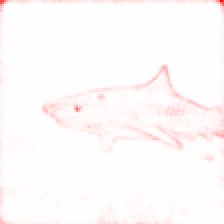
\includegraphics[width=\linewidth]{figures/experiments/saliency_quality/image_0018_ILSVRC2012_val_00034038.JPEG/zennit_lrp_gamma0.25_features_5_abs.png}
    \end{minipage}\hspace{0.002\linewidth}%
    \begin{minipage}[c]{0.10\linewidth}
        \centering
        
\includegraphics[width=\linewidth]{figures/experiments/saliency_quality/image_0018_ILSVRC2012_val_00034038.JPEG/hybrid_cam_shift_40_scale_max_winnerTakesItAllMaxpool_f14_cam_g.png}
    \end{minipage}\hspace{0.002\linewidth}%
    \begin{minipage}[c]{0.10\linewidth}
        \centering
        
\includegraphics[width=\linewidth]{figures/experiments/saliency_quality/image_0018_ILSVRC2012_val_00034038.JPEG/layer_cam_features_14_relu.png}
    \end{minipage}\hspace{0.002\linewidth}%
    \begin{minipage}[c]{0.10\linewidth}
        \centering
        
\includegraphics[width=\linewidth]{figures/experiments/saliency_quality/image_0018_ILSVRC2012_val_00034038.JPEG/hybrid_cam_shift_30_scale_max_winnerTakesItAllMaxpool_f26_cam_g_abs.png}
    \end{minipage}\hspace{0.002\linewidth}%
    \begin{minipage}[c]{0.10\linewidth}
        \centering
        
\includegraphics[width=\linewidth]{figures/experiments/saliency_quality/image_0018_ILSVRC2012_val_00034038.JPEG/layer_cam_features_26_relu.png}
    \end{minipage}\hspace{0.002\linewidth}%
    \begin{minipage}[c]{0.10\linewidth}
        \centering
        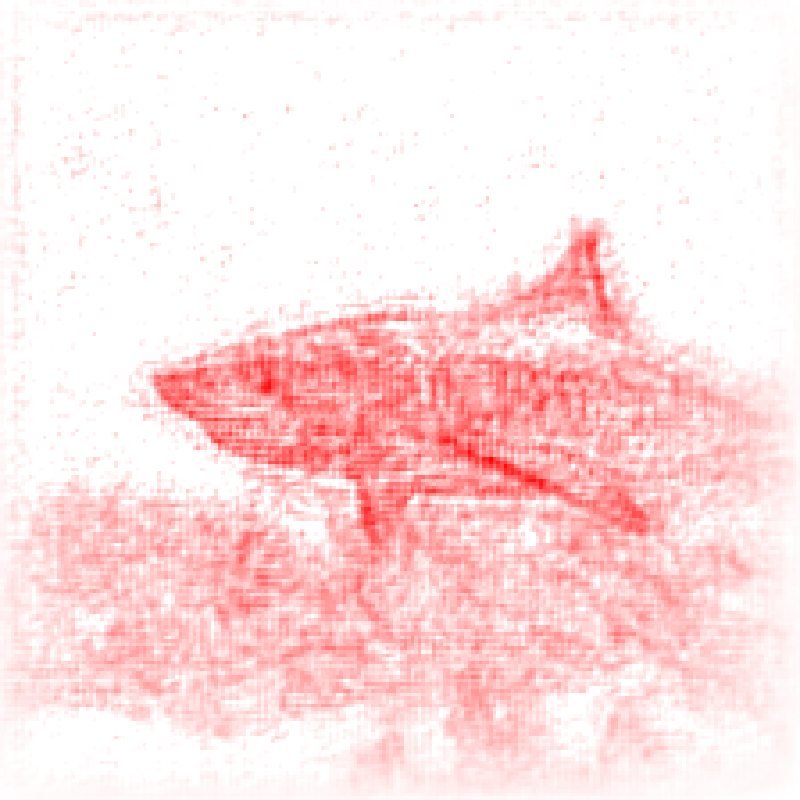
\includegraphics[width=\linewidth]{figures/experiments/saliency_quality/image_0018_ILSVRC2012_val_00034038.JPEG/hybrid_grad_shift_30_max_winnerTakesItAllMaxpool_f0_grad_pp.png}
    \end{minipage}%

    \vspace{0.3cm}

    \begin{minipage}[c]{0.08\linewidth}
        \centering
        \small goldfinch\\[1pt]
        {\scriptsize (1.0000)}
    \end{minipage}\hspace{0.002\linewidth}%
    \begin{minipage}[c]{0.10\linewidth}
        \centering
        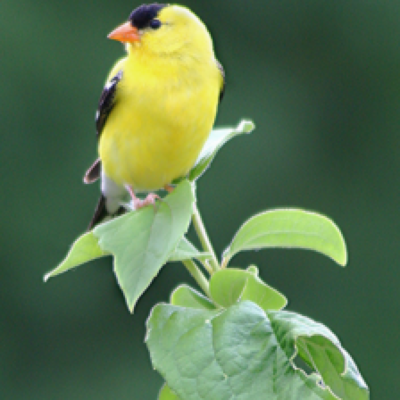
\includegraphics[width=\linewidth]{figures/experiments/saliency_quality/image_0034_ILSVRC2012_val_00044706.JPEG/original_image.png}
    \end{minipage}\hspace{0.002\linewidth}%
    \begin{minipage}[c]{0.10\linewidth}
        \centering
        
\includegraphics[width=\linewidth]{figures/experiments/saliency_quality/image_0034_ILSVRC2012_val_00044706.JPEG/hybrid_lrp_scaling_max_winnerTakesItAllMaxpool_f10_cam_pp_abs.png}
    \end{minipage}\hspace{0.002\linewidth}%
    \begin{minipage}[c]{0.10\linewidth}
        \centering
        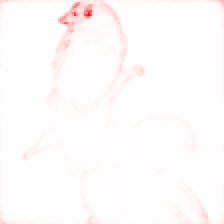
\includegraphics[width=\linewidth]{figures/experiments/saliency_quality/image_0034_ILSVRC2012_val_00044706.JPEG/zennit_lrp_gamma0.25_features_5_abs.png}
    \end{minipage}\hspace{0.002\linewidth}%
    \begin{minipage}[c]{0.10\linewidth}
        \centering
        
\includegraphics[width=\linewidth]{figures/experiments/saliency_quality/image_0034_ILSVRC2012_val_00044706.JPEG/hybrid_cam_shift_40_scale_max_winnerTakesItAllMaxpool_f14_cam_g.png}
    \end{minipage}\hspace{0.002\linewidth}%
    \begin{minipage}[c]{0.10\linewidth}
        \centering
        
\includegraphics[width=\linewidth]{figures/experiments/saliency_quality/image_0034_ILSVRC2012_val_00044706.JPEG/layer_cam_features_14_relu.png}
    \end{minipage}\hspace{0.002\linewidth}%
    \begin{minipage}[c]{0.10\linewidth}
        \centering
        
\includegraphics[width=\linewidth]{figures/experiments/saliency_quality/image_0034_ILSVRC2012_val_00044706.JPEG/hybrid_cam_shift_30_scale_max_winnerTakesItAllMaxpool_f26_cam_g_abs.png}
    \end{minipage}\hspace{0.002\linewidth}%
    \begin{minipage}[c]{0.10\linewidth}
        \centering
        
\includegraphics[width=\linewidth]{figures/experiments/saliency_quality/image_0034_ILSVRC2012_val_00044706.JPEG/layer_cam_features_26_relu.png}
    \end{minipage}\hspace{0.002\linewidth}%
    \begin{minipage}[c]{0.10\linewidth}
        \centering
        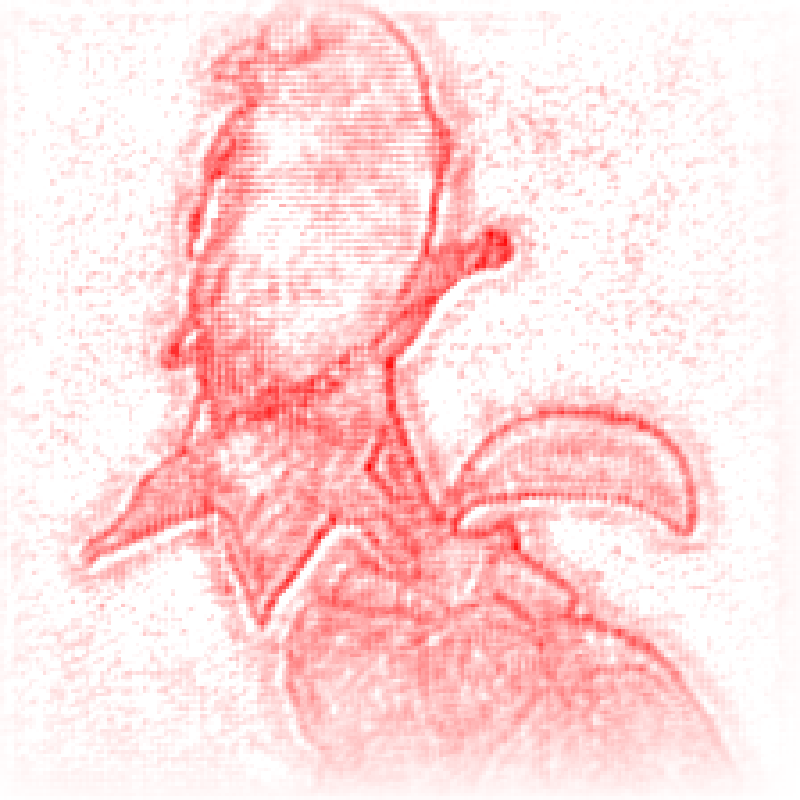
\includegraphics[width=\linewidth]{figures/experiments/saliency_quality/image_0034_ILSVRC2012_val_00044706.JPEG/hybrid_grad_shift_30_max_winnerTakesItAllMaxpool_f0_grad_pp.png}
    \end{minipage}%

    \vspace{0.3cm}

    \begin{minipage}[c]{0.08\linewidth}
        \centering
        \small tree frog\\[1pt]
        {\scriptsize (0.9954)}
    \end{minipage}\hspace{0.002\linewidth}%
    \begin{minipage}[c]{0.10\linewidth}
        \centering
        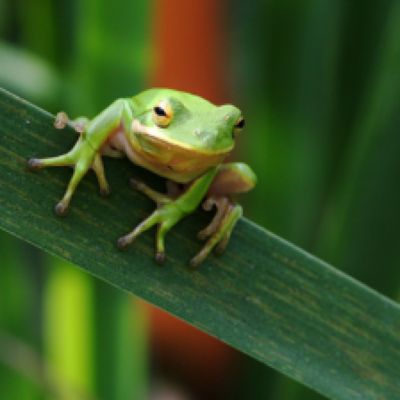
\includegraphics[width=\linewidth]{figures/experiments/saliency_quality/image_0041_ILSVRC2012_val_00017505.JPEG/original_image.png}
    \end{minipage}\hspace{0.002\linewidth}%
    \begin{minipage}[c]{0.10\linewidth}
        \centering
        
\includegraphics[width=\linewidth]{figures/experiments/saliency_quality/image_0041_ILSVRC2012_val_00017505.JPEG/hybrid_lrp_scaling_max_winnerTakesItAllMaxpool_f10_cam_pp_abs.png}
    \end{minipage}\hspace{0.002\linewidth}%
    \begin{minipage}[c]{0.10\linewidth}
        \centering
        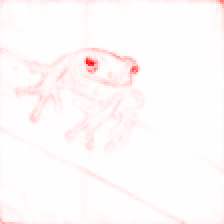
\includegraphics[width=\linewidth]{figures/experiments/saliency_quality/image_0041_ILSVRC2012_val_00017505.JPEG/zennit_lrp_gamma0.25_features_5_abs.png}
    \end{minipage}\hspace{0.002\linewidth}%
    \begin{minipage}[c]{0.10\linewidth}
        \centering
        
\includegraphics[width=\linewidth]{figures/experiments/saliency_quality/image_0041_ILSVRC2012_val_00017505.JPEG/hybrid_cam_shift_40_scale_max_winnerTakesItAllMaxpool_f14_cam_g.png}
    \end{minipage}\hspace{0.002\linewidth}%
    \begin{minipage}[c]{0.10\linewidth}
        \centering
        
\includegraphics[width=\linewidth]{figures/experiments/saliency_quality/image_0041_ILSVRC2012_val_00017505.JPEG/layer_cam_features_14_relu.png}
    \end{minipage}\hspace{0.002\linewidth}%
    \begin{minipage}[c]{0.10\linewidth}
        \centering
        
\includegraphics[width=\linewidth]{figures/experiments/saliency_quality/image_0041_ILSVRC2012_val_00017505.JPEG/hybrid_cam_shift_30_scale_max_winnerTakesItAllMaxpool_f26_cam_g_abs.png}
    \end{minipage}\hspace{0.002\linewidth}%
    \begin{minipage}[c]{0.10\linewidth}
        \centering
        
\includegraphics[width=\linewidth]{figures/experiments/saliency_quality/image_0041_ILSVRC2012_val_00017505.JPEG/layer_cam_features_26_relu.png}
    \end{minipage}\hspace{0.002\linewidth}%
    \begin{minipage}[c]{0.10\linewidth}
        \centering
        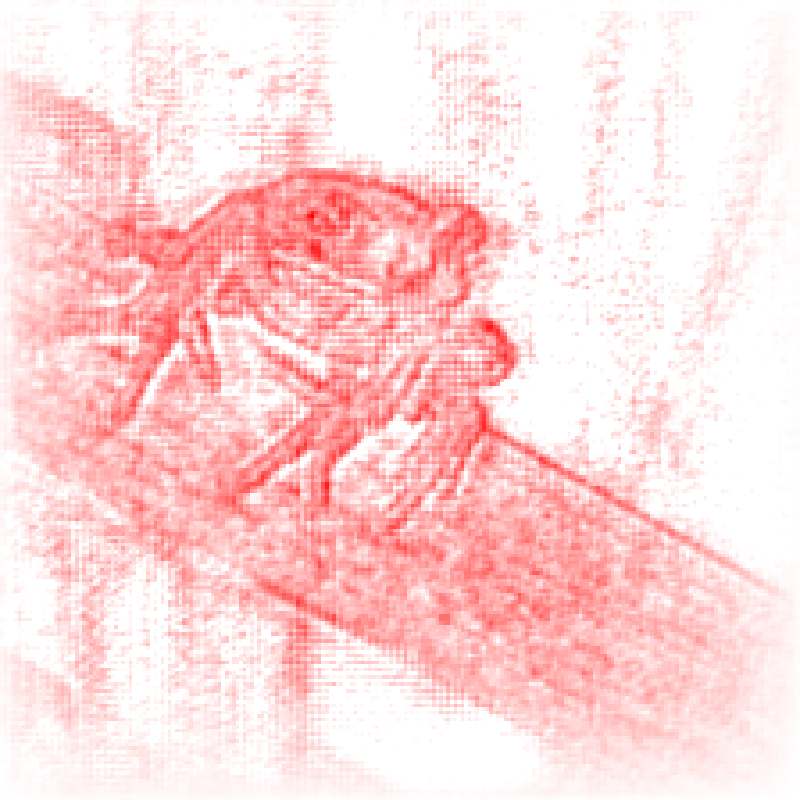
\includegraphics[width=\linewidth]{figures/experiments/saliency_quality/image_0041_ILSVRC2012_val_00017505.JPEG/hybrid_grad_shift_30_max_winnerTakesItAllMaxpool_f0_grad_pp.png}
    \end{minipage}%

    \vspace{0.3cm}

    \begin{minipage}[c]{0.08\linewidth}
        \centering
        \small ladybug\\[1pt]
        {\scriptsize (0.8272)}
    \end{minipage}\hspace{0.002\linewidth}%
    \begin{minipage}[c]{0.10\linewidth}
        \centering
        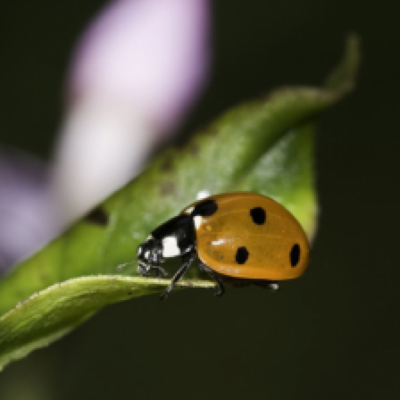
\includegraphics[width=\linewidth]{figures/experiments/saliency_quality/image_0096_ILSVRC2012_val_00025218.JPEG/original_image.png}
    \end{minipage}\hspace{0.002\linewidth}%
    \begin{minipage}[c]{0.10\linewidth}
        \centering
        
\includegraphics[width=\linewidth]{figures/experiments/saliency_quality/image_0096_ILSVRC2012_val_00025218.JPEG/hybrid_lrp_scaling_max_winnerTakesItAllMaxpool_f10_cam_pp_abs.png}
    \end{minipage}\hspace{0.002\linewidth}%
    \begin{minipage}[c]{0.10\linewidth}
        \centering
        
\includegraphics[width=\linewidth]{figures/experiments/saliency_quality/image_0096_ILSVRC2012_val_00025218.JPEG/zennit_lrp_gamma0.25_features_5_abs.png}
    \end{minipage}\hspace{0.002\linewidth}%
    \begin{minipage}[c]{0.10\linewidth}
        \centering
        
\includegraphics[width=\linewidth]{figures/experiments/saliency_quality/image_0096_ILSVRC2012_val_00025218.JPEG/hybrid_cam_shift_40_scale_max_winnerTakesItAllMaxpool_f14_cam_g.png}
    \end{minipage}\hspace{0.002\linewidth}%
    \begin{minipage}[c]{0.10\linewidth}
        \centering
        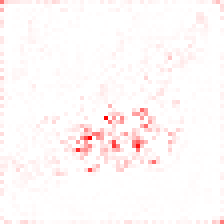
\includegraphics[width=\linewidth]{figures/experiments/saliency_quality/image_0096_ILSVRC2012_val_00025218.JPEG/layer_cam_features_14_relu.png}
    \end{minipage}\hspace{0.002\linewidth}%
    \begin{minipage}[c]{0.10\linewidth}
        \centering
        
\includegraphics[width=\linewidth]{figures/experiments/saliency_quality/image_0096_ILSVRC2012_val_00025218.JPEG/hybrid_cam_shift_30_scale_max_winnerTakesItAllMaxpool_f26_cam_g_abs.png}
    \end{minipage}\hspace{0.002\linewidth}%
    \begin{minipage}[c]{0.10\linewidth}
        \centering
        
\includegraphics[width=\linewidth]{figures/experiments/saliency_quality/image_0096_ILSVRC2012_val_00025218.JPEG/layer_cam_features_26_relu.png}
    \end{minipage}\hspace{0.002\linewidth}%
    \begin{minipage}[c]{0.10\linewidth}
        \centering
        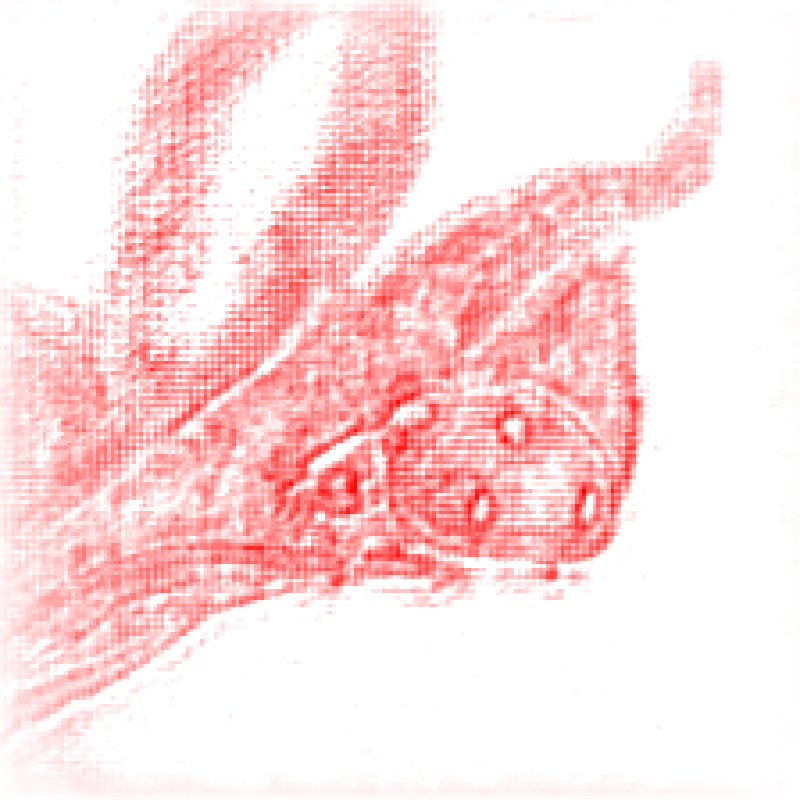
\includegraphics[width=\linewidth]{figures/experiments/saliency_quality/image_0096_ILSVRC2012_val_00025218.JPEG/hybrid_grad_shift_30_max_winnerTakesItAllMaxpool_f0_grad_pp.png}
    \end{minipage}%

    \vspace{0.3cm}

    \begin{minipage}[c]{0.08\linewidth}
        \centering
        \small wood rabbit\\[1pt]
        {\scriptsize (0.9782)}
    \end{minipage}\hspace{0.002\linewidth}%
    \begin{minipage}[c]{0.10\linewidth}
        \centering
        
\includegraphics[width=\linewidth]{figures/experiments/saliency_quality/image_0120_ILSVRC2012_val_00024858.JPEG/original_image.png}
    \end{minipage}\hspace{0.002\linewidth}%
    \begin{minipage}[c]{0.10\linewidth}
        \centering
        
\includegraphics[width=\linewidth]{figures/experiments/saliency_quality/image_0120_ILSVRC2012_val_00024858.JPEG/hybrid_lrp_scaling_max_winnerTakesItAllMaxpool_f10_cam_pp_abs.png}
    \end{minipage}\hspace{0.002\linewidth}%
    \begin{minipage}[c]{0.10\linewidth}
        \centering
        
\includegraphics[width=\linewidth]{figures/experiments/saliency_quality/image_0120_ILSVRC2012_val_00024858.JPEG/zennit_lrp_gamma0.25_features_5_abs.png}
    \end{minipage}\hspace{0.002\linewidth}%
    \begin{minipage}[c]{0.10\linewidth}
        \centering
        
\includegraphics[width=\linewidth]{figures/experiments/saliency_quality/image_0120_ILSVRC2012_val_00024858.JPEG/hybrid_cam_shift_40_scale_max_winnerTakesItAllMaxpool_f14_cam_g.png}
    \end{minipage}\hspace{0.002\linewidth}%
    \begin{minipage}[c]{0.10\linewidth}
        \centering
        
\includegraphics[width=\linewidth]{figures/experiments/saliency_quality/image_0120_ILSVRC2012_val_00024858.JPEG/layer_cam_features_14_relu.png}
    \end{minipage}\hspace{0.002\linewidth}%
    \begin{minipage}[c]{0.10\linewidth}
        \centering
        
\includegraphics[width=\linewidth]{figures/experiments/saliency_quality/image_0120_ILSVRC2012_val_00024858.JPEG/hybrid_cam_shift_30_scale_max_winnerTakesItAllMaxpool_f26_cam_g_abs.png}
    \end{minipage}\hspace{0.002\linewidth}%
    \begin{minipage}[c]{0.10\linewidth}
        \centering
        
\includegraphics[width=\linewidth]{figures/experiments/saliency_quality/image_0120_ILSVRC2012_val_00024858.JPEG/layer_cam_features_26_relu.png}
    \end{minipage}\hspace{0.002\linewidth}%
    \begin{minipage}[c]{0.10\linewidth}
        \centering
        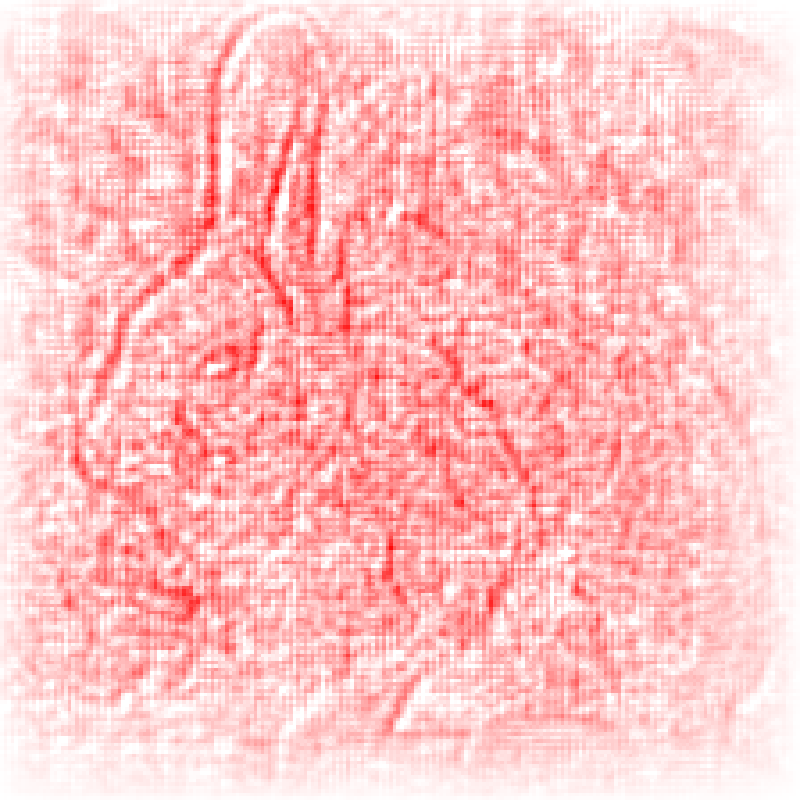
\includegraphics[width=\linewidth]{figures/experiments/saliency_quality/image_0120_ILSVRC2012_val_00024858.JPEG/hybrid_grad_shift_30_max_winnerTakesItAllMaxpool_f0_grad_pp.png}
    \end{minipage}%

    \vspace{0.3cm}

    \begin{minipage}[c]{0.08\linewidth}
        \centering
        \small water tower\\[1pt]
        {\scriptsize (1.0000)}
    \end{minipage}\hspace{0.002\linewidth}%
    \begin{minipage}[c]{0.10\linewidth}
        \centering
        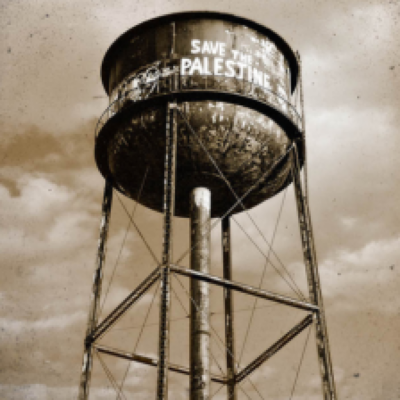
\includegraphics[width=\linewidth]{figures/experiments/saliency_quality/image_0499_ILSVRC2012_val_00037082.JPEG/original_image.png}
    \end{minipage}\hspace{0.002\linewidth}%
    \begin{minipage}[c]{0.10\linewidth}
        \centering
        
\includegraphics[width=\linewidth]{figures/experiments/saliency_quality/image_0499_ILSVRC2012_val_00037082.JPEG/hybrid_lrp_scaling_max_winnerTakesItAllMaxpool_f10_cam_pp_abs.png}
    \end{minipage}\hspace{0.002\linewidth}%
    \begin{minipage}[c]{0.10\linewidth}
        \centering
        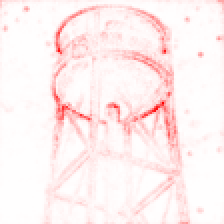
\includegraphics[width=\linewidth]{figures/experiments/saliency_quality/image_0499_ILSVRC2012_val_00037082.JPEG/zennit_lrp_gamma0.25_features_5_abs.png}
    \end{minipage}\hspace{0.002\linewidth}%
    \begin{minipage}[c]{0.10\linewidth}
        \centering
        
\includegraphics[width=\linewidth]{figures/experiments/saliency_quality/image_0499_ILSVRC2012_val_00037082.JPEG/hybrid_cam_shift_40_scale_max_winnerTakesItAllMaxpool_f14_cam_g.png}
    \end{minipage}\hspace{0.002\linewidth}%
    \begin{minipage}[c]{0.10\linewidth}
        \centering
        
\includegraphics[width=\linewidth]{figures/experiments/saliency_quality/image_0499_ILSVRC2012_val_00037082.JPEG/layer_cam_features_14_relu.png}
    \end{minipage}\hspace{0.002\linewidth}%
    \begin{minipage}[c]{0.10\linewidth}
        \centering
        
\includegraphics[width=\linewidth]{figures/experiments/saliency_quality/image_0499_ILSVRC2012_val_00037082.JPEG/hybrid_cam_shift_30_scale_max_winnerTakesItAllMaxpool_f26_cam_g_abs.png}
    \end{minipage}\hspace{0.002\linewidth}%
    \begin{minipage}[c]{0.10\linewidth}
        \centering
        
\includegraphics[width=\linewidth]{figures/experiments/saliency_quality/image_0499_ILSVRC2012_val_00037082.JPEG/layer_cam_features_26_relu.png}
    \end{minipage}\hspace{0.002\linewidth}%
    \begin{minipage}[c]{0.10\linewidth}
        \centering
        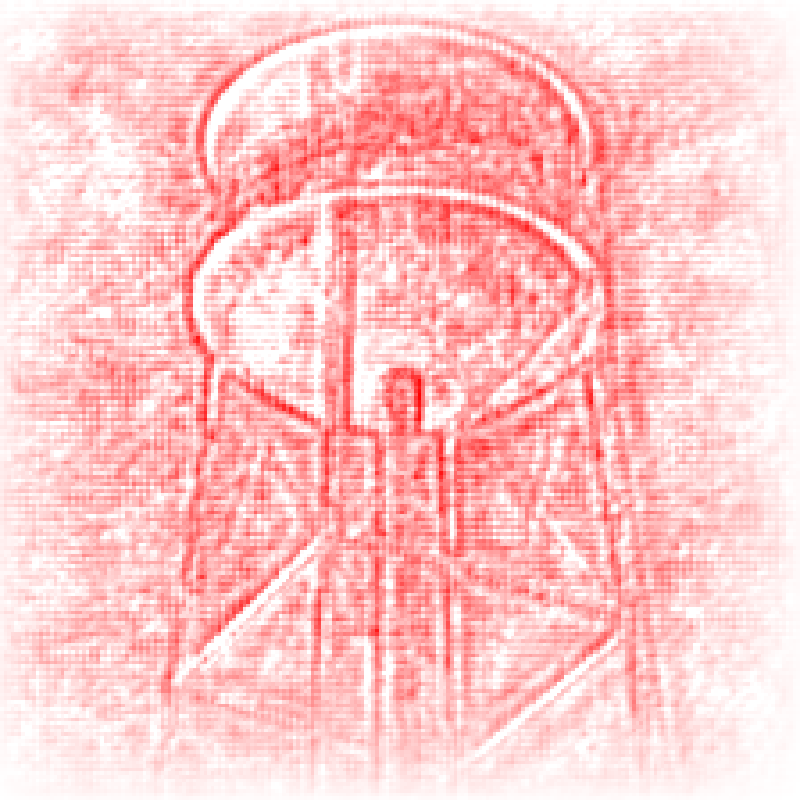
\includegraphics[width=\linewidth]{figures/experiments/saliency_quality/image_0499_ILSVRC2012_val_00037082.JPEG/hybrid_grad_shift_30_max_winnerTakesItAllMaxpool_f0_grad_pp.png}
    \end{minipage}%

    \vspace{0.3cm}

    \begin{minipage}[c]{0.08\linewidth}
        \centering
        \small yawl\\[1pt]
        {\scriptsize (0.9953)}
    \end{minipage}\hspace{0.002\linewidth}%
    \begin{minipage}[c]{0.10\linewidth}
        \centering
        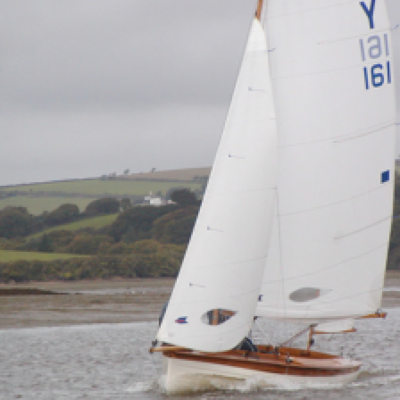
\includegraphics[width=\linewidth]{figures/experiments/saliency_quality/image_0511_ILSVRC2012_val_00035734.JPEG/original_image.png}
    \end{minipage}\hspace{0.002\linewidth}%
    \begin{minipage}[c]{0.10\linewidth}
        \centering
        
\includegraphics[width=\linewidth]{figures/experiments/saliency_quality/image_0511_ILSVRC2012_val_00035734.JPEG/hybrid_lrp_scaling_max_winnerTakesItAllMaxpool_f10_cam_pp_abs.png}
    \end{minipage}\hspace{0.002\linewidth}%
    \begin{minipage}[c]{0.10\linewidth}
        \centering
        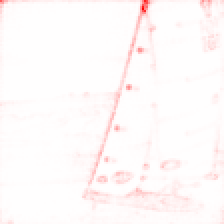
\includegraphics[width=\linewidth]{figures/experiments/saliency_quality/image_0511_ILSVRC2012_val_00035734.JPEG/zennit_lrp_gamma0.25_features_5_abs.png}
    \end{minipage}\hspace{0.002\linewidth}%
    \begin{minipage}[c]{0.10\linewidth}
        \centering
        
\includegraphics[width=\linewidth]{figures/experiments/saliency_quality/image_0511_ILSVRC2012_val_00035734.JPEG/hybrid_cam_shift_40_scale_max_winnerTakesItAllMaxpool_f14_cam_g.png}
    \end{minipage}\hspace{0.002\linewidth}%
    \begin{minipage}[c]{0.10\linewidth}
        \centering
        
\includegraphics[width=\linewidth]{figures/experiments/saliency_quality/image_0511_ILSVRC2012_val_00035734.JPEG/layer_cam_features_14_relu.png}
    \end{minipage}\hspace{0.002\linewidth}%
    \begin{minipage}[c]{0.10\linewidth}
        \centering
        
\includegraphics[width=\linewidth]{figures/experiments/saliency_quality/image_0511_ILSVRC2012_val_00035734.JPEG/hybrid_cam_shift_30_scale_max_winnerTakesItAllMaxpool_f26_cam_g_abs.png}
    \end{minipage}\hspace{0.002\linewidth}%
    \begin{minipage}[c]{0.10\linewidth}
        \centering
        
\includegraphics[width=\linewidth]{figures/experiments/saliency_quality/image_0511_ILSVRC2012_val_00035734.JPEG/layer_cam_features_26_relu.png}
    \end{minipage}\hspace{0.002\linewidth}%
    \begin{minipage}[c]{0.10\linewidth}
        \centering
        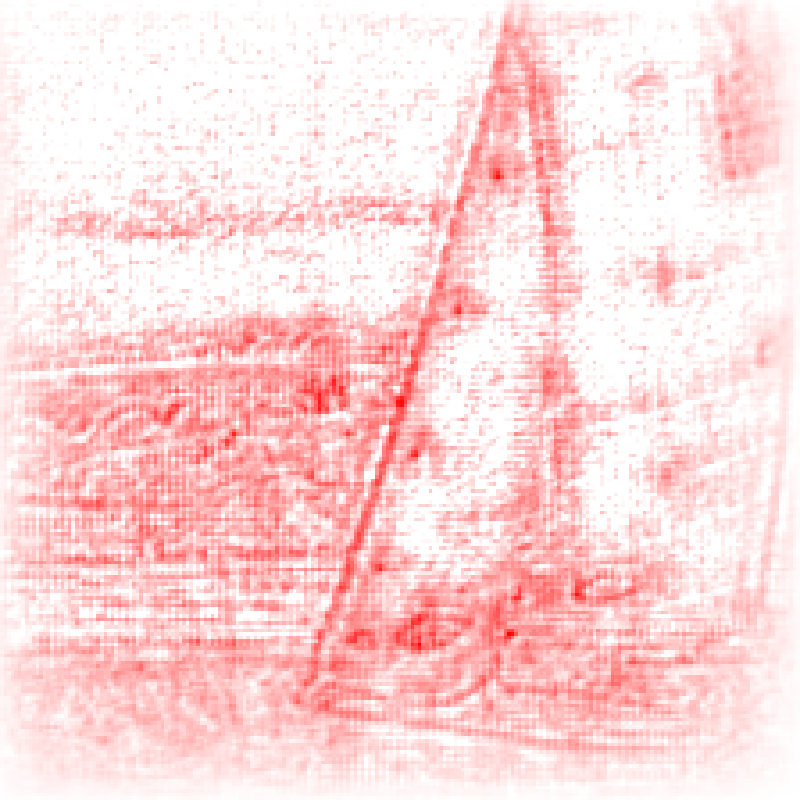
\includegraphics[width=\linewidth]{figures/experiments/saliency_quality/image_0511_ILSVRC2012_val_00035734.JPEG/hybrid_grad_shift_30_max_winnerTakesItAllMaxpool_f0_grad_pp.png}
    \end{minipage}%

    }%
\caption[Additional VGG-16 saliency map comparisons]{Saliency map comparison for VGG-16 on images from the custom ImageNet-S test subset. Each row shows the predicted class (with confidence), original image, and saliency maps from different methods. Methods include SplitLRP, classical LRP, SplitCAM variants, LayerCAM, and SplitGrad. Notation follows Figure~\ref{fig:vgg_saliency_comparison_main}.}
    \label{fig:vgg_saliency_comparison}
\end{figure}


\subsection{Quantitative Analysis on VGG-16}\label{app:vgg_split}

Table~\ref{tab:xai_eval_comprehensive_vgg} contains the comprehensive VGG-16 comparison discussed in Section~\ref{sec:results_vgg}. Selected rows can differ in layer and absolute-value convention; the controlled $\alpha$ sweeps below isolate these choices more directly.

% Source: hiddenMonotonicity (Paper 1), appendix/table_appendix_generated_vgg_full_eval_sorted.tex — numbers verbatim.
\begingroup
\small
\setlength{\tabcolsep}{3pt}
\renewcommand{\arraystretch}{1.05}
\LongTableContent{
\caption[Comprehensive interpretability evaluation: VGG-16]{Comprehensive interpretability evaluation results (VGG-16; representative configurations, best per method). \emph{wta} denotes winner-take-all max-pooling, and \emph{sc} forward scaling (Section~\ref{sec:stabilization_dc}); layer brackets follow the split-method upper indices of Section~\ref{sec:split_attribution_concept}. Within each block, the best value of each metric is bold with dark blue shading; a rule separates the configurations of one method, whose rows differ in the attribution layer. PF$^{\mathrm{drop}}$ is score-drop AUC; n/r denotes a result not reported in the paper, and n/a an inapplicable entry. Attribution Localization is computed on the signed maps unless \emph{Abs} is set, so it can be negative; the original-image baseline uses the normalized input as its map.}
    \label{tab:xai_eval_comprehensive_vgg}%
}{%
\begin{longtable}{@{}>{\raggedright\arraybackslash}p{3.6cm}cc cccccc@{}}
    \TableHeading \\
    \toprule
    Method & Layer & Abs & Sel$\downarrow$ & AL$\uparrow$ & PG$\uparrow$ & PF$^{\mathrm{drop}}_5$$\uparrow$ & PF$^{\mathrm{drop}}_{20}$$\uparrow$ & MaxS$\downarrow$ \\
    \midrule
    \endfirsthead

    \multicolumn{9}{c}%
    {{\tablename\ \thetable{} -- continued from previous page}} \\
    \toprule
    Method & Layer & Abs & Sel$\downarrow$ & AL$\uparrow$ & PG$\uparrow$ & PF$^{\mathrm{drop}}_5$$\uparrow$ & PF$^{\mathrm{drop}}_{20}$$\uparrow$ & MaxS$\downarrow$ \\
    \midrule
    \endhead

    \midrule
    \multicolumn{9}{r}{{Continued on next page}} \\
    \midrule
    \endfoot

    \bottomrule
    \endlastfoot

    \multicolumn{9}{c}{\textit{SplitCAM Methods}} \\
    \midrule
    SplitCAM (sc, $\alpha \ 0.4$) & (12, g) & n & 4.720 & \cellbest{\textbf{0.651}} & 0.912 & 0.213 & 1.794 & \cellbest{\textbf{0.389}} \\
    SplitCAM (sc, $\alpha \ 0.4$) & (14, g) & n & \cellbest{\textbf{2.727}} & 0.563 & 0.836 & 0.300 & 2.404 & 1.012 \\
    \cmidrule(lr){1-9}
    SplitCAM (sc, $\alpha \ 0.4$, wta) & (14, g) & n & 2.761 & 0.543 & 0.827 & \cellbest{\textbf{0.303}} & 2.414 & 1.056 \\
    SplitCAM (sc, $\alpha \ 0.4$, wta) & (26, +, g) & y & 4.711 & 0.635 & \cellbest{\textbf{0.938}} & 0.165 & 1.590 & 0.456 \\
    \cmidrule(lr){1-9}
    SplitCAM (sc, $\alpha \ 0.5$, wta) & (14, g) & n & 2.766 & 0.536 & 0.823 & \cellbest{\textbf{0.303}} & \cellbest{\textbf{2.416}} & 1.056 \\
    SplitCAM (sc, $\alpha \ 0.5$, wta) & (26, +, g) & n & 4.608 & 0.607 & 0.903 & 0.185 & 1.684 & 0.566 \\
    \midrule
    \multicolumn{9}{c}{\textit{SplitGrad Methods}} \\
    \midrule
    SplitGrad ($\alpha \ 0.4$) & (12, +, g) & n & 5.633 & 0.613 & 0.873 & 0.148 & 1.461 & \cellbest{\textbf{0.364}} \\
    SplitGrad ($\alpha \ 0.4$) & (14, +, g) & y & 3.429 & 0.533 & 0.820 & 0.235 & 2.119 & 0.851 \\
    \cmidrule(lr){1-9}
    SplitGrad ($\alpha \ 0.4$, wta) & (12, +, g) & n & 4.735 & \cellbest{\textbf{0.635}} & 0.883 & 0.186 & 1.756 & 0.651 \\
    SplitGrad ($\alpha \ 0.4$, wta) & (14, +, g) & y & \cellbest{\textbf{3.287}} & 0.540 & 0.818 & 0.249 & 2.186 & 0.857 \\
    \cmidrule(lr){1-9}
    SplitGrad ($\alpha \ 0.5$, wta) & (12, +, g) & y & 3.379 & 0.551 & 0.859 & \cellbest{\textbf{0.261}} & \cellbest{\textbf{2.220}} & 0.869 \\
    SplitGrad ($\alpha \ 0.5$, wta) & (26, g) & y & 4.948 & 0.543 & \cellbest{\textbf{0.899}} & 0.162 & 1.527 & 0.617 \\
    \midrule
    \multicolumn{9}{c}{\textit{SplitLRP Methods}} \\
    \midrule
    SplitLRP (sc) & (7, pos) & n & \cellbest{\textbf{3.062}} & 0.092 & 0.857 & \cellbest{\textbf{0.296}} & 2.290 & 0.865 \\
    SplitLRP (sc) & (19, pos) & n & 4.393 & \cellbest{\textbf{0.600}} & 0.823 & 0.166 & 1.656 & 0.291 \\
    \cmidrule(lr){1-9}
    SplitLRP (sc, wta) & (7, pos) & n & 3.235 & -0.036 & 0.836 & \cellbest{\textbf{0.296}} & \cellbest{\textbf{2.291}} & 0.866 \\
    SplitLRP (sc, wta) & (26, pos) & y & 5.168 & 0.588 & \cellbest{\textbf{0.871}} & 0.151 & 1.473 & \cellbest{\textbf{0.282}} \\
    \midrule
    \multicolumn{9}{c}{\textit{Classical Methods (No Layer Optimization)}} \\
    \midrule
    Deconvolution & 0 & y & 5.435 & 0.468 & 0.629 & 0.204 & 1.715 & 0.956 \\
    DeepLIFT & 0 & y & \cellbest{\textbf{4.447}} & 0.551 & 0.726 & \cellbest{\textbf{0.281}} & \cellbest{\textbf{1.945}} & 1.053 \\
    Feature Ablation & 0 & y & 6.029 & 0.479 & 0.624 & 0.123 & 1.250 & 0.859 \\
    GradientSHAP & 0 & y & 4.808 & 0.552 & 0.783 & 0.261 & 1.862 & 1.142 \\
    IntGrad & 0 & y & 4.838 & 0.554 & 0.797 & 0.262 & 1.851 & 1.069 \\
    Occlusion & 0 & y & 5.214 & 0.499 & 0.716 & 0.130 & 1.217 & 0.699 \\
    GCAM++ & 30 & n & 5.955 & \cellbest{\textbf{0.564}} & \cellbest{\textbf{0.827}} & 0.130 & 1.245 & \cellbest{\textbf{0.401}} \\
    \midrule
    \multicolumn{9}{c}{\textit{Classical Methods (Layer Optimization)}} \\
    \midrule
    Guided Backprop & 2 & n & 3.276 & \cellbest{\textbf{0.632}} & 0.883 & 0.281 & 2.302 & 0.571 \\
    Guided Backprop & 5 & n & 3.448 & 0.614 & \cellbest{\textbf{0.887}} & 0.240 & 2.091 & \cellbest{\textbf{0.375}} \\
    \cmidrule(lr){1-9}
    Guided GCAM & 0 & n & 4.301 & -0.053 & 0.857 & 0.161 & 1.459 & 1.047 \\
    Guided GCAM & 26 & n & 5.130 & -2.635 & 0.843 & 0.179 & 1.415 & 0.947 \\
    \cmidrule(lr){1-9}
    GCAM & 0 & n & 6.006 & 0.356 & 0.638 & 0.060 & 0.899 & 1.123 \\
    GCAM & 14 & n & 5.555 & 0.306 & 0.580 & 0.136 & 1.525 & 0.903 \\
    \cmidrule(lr){1-9}
    LCAM & 14 & n/a & \cellbest{\textbf{2.792}} & 0.576 & 0.798 & \cellbest{\textbf{0.317}} & \cellbest{\textbf{2.474}} & 2.656 \\
    LCAM & 2 & n/a & 3.128 & 0.580 & 0.855 & 0.300 & 2.191 & 5.508 \\
    \cmidrule(lr){1-9}
    LRP $\gamma=0.25$ & 0 & n & 3.189 & 0.615 & 0.680 & 0.218 & 1.918 & 0.519 \\
    LRP $\gamma=0.25$ & 14 & n & 3.593 & 0.577 & 0.611 & 0.279 & 2.255 & 0.491 \\
    \midrule
    \multicolumn{9}{c}{\textit{Baseline Methods}} \\
    \midrule
    Baseline: Binary Mask & 0 & y & 6.011 & \cellbest{\textbf{1.000}} & \cellbest{\textbf{1.000}} & 0.091 & 1.054 & n/r \\
    Baseline: Original Image & 0 & n & 8.770 & -1.699 & 0.572 & 0.061 & 0.619 & n/r \\
    Random Baseline & 0 & y & \cellbest{\textbf{3.570}} & 0.425 & 0.458 & \cellbest{\textbf{0.203}} & \cellbest{\textbf{1.585}} & n/r \\
    \midrule
\end{longtable}%
}
\endgroup


\subsection{Quantitative Analysis on ResNet-18}\label{app:resnet_split}

Table~\ref{tab:xai_eval_comprehensive_res} presents detailed quantitative metrics across all split configurations, baselines, and classical methods for ResNet-18.

% Source: hiddenMonotonicity (Paper 1), appendix/table_appendix_generated_res_full_eval_sorted.tex — numbers verbatim.
% Note: the paper's appendix caption said "ResNet50"; the evaluated model is the ResNet18 of the
% main results (cf. tab:eval_res_main and the paper's main text), so the caption is corrected here.
\begingroup
\fontsize{8.5}{10}\selectfont
\setlength{\tabcolsep}{3pt}
\renewcommand{\arraystretch}{1.05}
\LongTableContent{
\caption[Comprehensive interpretability evaluation: ResNet-18]{Comprehensive interpretability evaluation results (ResNet-18; representative configurations, best per method). Abbreviations as in Table~\ref{tab:xai_eval_comprehensive_vgg}; triples $x.y.z$ identify the internal convolutional attribution layer. For each method configuration the best metric values across the considered layer configurations are highlighted in bold with dark blue shading. PF$^{\mathrm{drop}}$ is score-drop AUC; n/r denotes a result not reported in the paper, and n/a an inapplicable entry. Attribution Localization is computed on the signed maps unless \emph{Abs} is set, so it can be negative; the original-image baseline uses the normalized input as its map.}
    \label{tab:xai_eval_comprehensive_res}%
}{%
\begin{longtable}{@{}>{\raggedright\arraybackslash}p{3.6cm}cc cccccc@{}}
    \TableHeading \\
    \toprule
    Method & Layer & Abs & Sel$\downarrow$ & AL$\uparrow$ & PG$\uparrow$ & PF$^{\mathrm{drop}}_5$$\uparrow$ & PF$^{\mathrm{drop}}_{20}$$\uparrow$ & MaxS$\downarrow$ \\
    \midrule
    \endfirsthead

    \multicolumn{9}{c}%
    {{\tablename\ \thetable{} -- continued from previous page}} \\
    \toprule
    Method & Layer & Abs & Sel$\downarrow$ & AL$\uparrow$ & PG$\uparrow$ & PF$^{\mathrm{drop}}_5$$\uparrow$ & PF$^{\mathrm{drop}}_{20}$$\uparrow$ & MaxS$\downarrow$ \\
    \midrule
    \endhead

    \midrule
    \multicolumn{9}{r}{{Continued on next page}} \\
    \midrule
    \endfoot

    \bottomrule
    \endlastfoot

    \multicolumn{9}{c}{\textit{SplitCAM Methods}} \\
    \midrule
    SplitCAM (sc, $\alpha\ 0.3$, wta) & (1.0.2, g) & n & \cellbest{\textbf{3.503}} & 0.487 & 0.747 & \cellbest{\textbf{0.168}} & \cellbest{\textbf{1.395}} & 1.277 \\
    SplitCAM (sc, $\alpha\ 0.3$, wta) & (4.1.2, g) & n & 5.654 & \cellbest{\textbf{0.673}} & \cellbest{\textbf{0.972}} & 0.081 & 0.880 & \cellbest{\textbf{0.233}} \\
    \cmidrule(lr){1-9}
    SplitCAM (sc, $\alpha\ 0.5$, wta) & (2.0.1, g) & n & \cellbest{\textbf{3.682}} & -1.370 & 0.887 & \cellbest{\textbf{0.158}} & \cellbest{\textbf{1.447}} & 1.078 \\
    SplitCAM (sc, $\alpha\ 0.5$, wta) & (4.1.1, +, g) & y & 6.526 & \cellbest{\textbf{0.611}} & \cellbest{\textbf{0.956}} & 0.066 & 0.737 & \cellbest{\textbf{0.187}} \\
    \midrule
    \multicolumn{9}{c}{\textit{SplitGrad Methods}} \\
    \midrule
    SplitGrad ($\alpha\ 0.3$, wta) & (1.0.2, g) & y & \cellbest{\textbf{4.449}} & 0.513 & 0.777 & \cellbest{\textbf{0.149}} & \cellbest{\textbf{1.266}} & 0.813 \\
    SplitGrad ($\alpha\ 0.3$, wta) & (4.1.2, g) & y & 5.663 & \cellbest{\textbf{0.649}} & \cellbest{\textbf{0.972}} & 0.082 & 0.882 & \cellbest{\textbf{0.219}} \\
    \cmidrule(lr){1-9}
    SplitGrad ($\alpha\ 0.5$, wta) & (3.1.1, g) & y & \cellbest{\textbf{3.588}} & 0.559 & 0.880 & \cellbest{\textbf{0.130}} & \cellbest{\textbf{1.366}} & 0.859 \\
    SplitGrad ($\alpha\ 0.5$, wta) & (4.1.2, g) & y & 5.690 & \cellbest{\textbf{0.654}} & \cellbest{\textbf{0.972}} & 0.083 & 0.886 & \cellbest{\textbf{0.230}} \\
    \midrule
    \multicolumn{9}{c}{\textit{SplitLRP Methods}} \\
    \midrule
    SplitLRP (sc, wta) & (conv1, pos) & y & \cellbest{\textbf{6.313}} & \cellbest{\textbf{0.506}} & \cellbest{\textbf{0.587}} & \cellbest{\textbf{0.056}} & \cellbest{\textbf{0.697}} & 0.755 \\
    SplitLRP (sc, wta) & (1.0.2, pos) & y & 6.785 & 0.483 & 0.567 & 0.050 & 0.686 & \cellbest{\textbf{0.696}} \\
    \midrule
    \multicolumn{9}{c}{\textit{Classical Methods (No Layer Optimization)}} \\
    \midrule
    Deconvolution & conv1 & y & 5.474 & 0.478 & 0.666 & 0.151 & 1.177 & 0.618 \\
    GradientSHAP & conv1 & y & 5.269 & 0.527 & 0.779 & 0.166 & 1.227 & 1.074 \\
    GCAM++ & 4.1.2 & n & 6.054 & 0.556 & 0.945 & 0.077 & 0.838 & 0.140 \\
    IntGrad & conv1 & y & 5.265 & 0.528 & 0.777 & 0.167 & 1.226 & 0.994 \\
    Feature Ablation & conv1 & n & 4.655 & 0.136 & 0.684 & 0.188 & 1.388 & 1.077 \\
    Occlusion & conv1 & n & 5.300 & 0.179 & 0.726 & 0.130 & 1.030 & 0.785 \\
    Deconvolution & conv1 & n & 3.934 & 0.484 & 0.666 & 0.147 & 1.203 & 0.751 \\
    \midrule
    \multicolumn{9}{c}{\textit{Classical Methods (Layer Optimization)}} \\
    \midrule
    GCAM & 2.0.1 & y & \cellbest{\textbf{4.003}} & 0.450 & 0.678 & 0.052 & \cellbest{\textbf{1.024}} & 0.738 \\
    GCAM & 4.1.2 & n & 6.070 & \cellbest{\textbf{0.554}} & \cellbest{\textbf{0.945}} & \cellbest{\textbf{0.076}} & 0.829 & \cellbest{\textbf{0.131}} \\
    \cmidrule(lr){1-9}
    Guided GCAM & 4.0.2 & n & 4.929 & \cellbest{\textbf{0.742}} & 0.866 & 0.119 & 1.008 & 0.687 \\
    Guided GCAM & 4.1.2 & n & \cellbest{\textbf{3.843}} & 0.717 & \cellbest{\textbf{0.883}} & \cellbest{\textbf{0.129}} & \cellbest{\textbf{1.096}} & \cellbest{\textbf{0.612}} \\
    \cmidrule(lr){1-9}
    LCAM & 2.0.2 & n & \cellbest{\textbf{3.690}} & 0.549 & 0.865 & \cellbest{\textbf{0.144}} & \cellbest{\textbf{1.428}} & 0.913 \\
    LCAM & 4.1.1 & n & 5.661 & \cellbest{\textbf{0.664}} & \cellbest{\textbf{0.971}} & 0.083 & 0.890 & \cellbest{\textbf{0.227}} \\
    \cmidrule(lr){1-9}
    LRP $\gamma=0.25$ & conv1 & y & \cellbest{\textbf{3.550}} & \cellbest{\textbf{0.656}} & 0.852 & \cellbest{\textbf{0.213}} & \cellbest{\textbf{1.737}} & 0.521 \\
    LRP $\gamma=0.25$ & 4.1.1 & n & 5.649 & 0.630 & \cellbest{\textbf{0.965}} & 0.081 & 0.877 & \cellbest{\textbf{0.200}} \\
    \cmidrule(lr){1-9}
    Guided Backprop & conv1 & n & \cellbest{\textbf{3.517}} & \cellbest{\textbf{0.621}} & 0.867 & \cellbest{\textbf{0.212}} & \cellbest{\textbf{1.757}} & 0.459 \\
    Guided Backprop & 3.1.2 & n & 3.874 & 0.582 & \cellbest{\textbf{0.938}} & 0.121 & 1.307 & \cellbest{\textbf{0.213}} \\
    \midrule
    \multicolumn{9}{c}{\textit{Baseline Methods}} \\
    \midrule
    Baseline: Original Image & conv1 & n & 8.351 & -1.699 & 0.572 & 0.049 & 0.435 & n/r \\
    Baseline: Binary Mask & conv1 & y & 5.964 & 1.000 & 1.000 & 0.067 & 0.739 & n/r \\
    Random Baseline & n/a & y & 4.071 & 0.425 & 0.440 & 0.147 & 1.067 & n/r \\
    \midrule
    \end{longtable}%
}
\endgroup


\section{Split-Method Randomization Sanity Check}\label{app:p1_sanity}

The model-randomization sanity check~\parencite{Adebayo2018sanity} tests dependence on learned parameters versus input patterns surviving model corruption. For each method, maps from trained VGG-16 are compared with maps after Gaussian reinitialization of the last three fully connected layers; parameter-sensitive methods should show a substantial similarity drop. Section~\ref{subsec:hellinger_randomization} extends randomization testing to the underlying trajectory distributions. Similarity measures are (i)~HOG similarity (Pearson correlation of histograms of oriented gradients), (ii)~signed Spearman rank correlation, and (iii)~SSIM; lower similarity indicates stronger parameter dependence.

% Source: hiddenMonotonicity (Paper 1), appendix/randomization_sanity_check_table.tex — numbers verbatim.
\begin{table}[htbp]
\centering
\caption[Randomization sanity check for VGG-16 split methods]{Randomization sanity check for the split methods on VGG-16: mean similarity between attribution maps of the trained model and of a copy whose last three fully connected layers are randomly reinitialized, across the custom test subset of ImageNet-S. Lower similarity indicates stronger dependence on the learned parameters; within each block, the lowest value of each metric is bold with dark blue shading. Abbreviations as in Table~\ref{tab:eval_vgg_main}.}
\label{tab:randomization_sanity_check}
\TableContent{
\small
\begin{adjustbox}{max width=\linewidth}
\begin{tabular}{l c c c}
\toprule
Method & HOG $\downarrow$ & Spearman $\downarrow$ & SSIM $\downarrow$ \\
\midrule
\multicolumn{4}{l}{\textbf{Baselines}} \\
Deconvolution & 0.985 & 0.999 & 0.481 \\
DeepLIFT & 0.365 & 0.274 & 0.716 \\
GradientSHAP & 0.286 & \cellbest{\textbf{0.081}} & 0.571 \\
Input $\times$ Gradient & 0.313 & 0.082 & 0.621 \\
IntGrad & 0.303 & 0.102 & 0.584 \\
LCAM (layer 14) & 0.688 & 0.123 & 0.417 \\
LCAM (layer 2) & 0.542 & 0.114 & 0.475 \\
Saliency & \cellbest{\textbf{0.188}} & 0.416 & \cellbest{\textbf{0.353}} \\
\midrule
\multicolumn{4}{l}{\textbf{SplitCAM}} \\
SplitCAM (sc, $\alpha = 0.4$) (12, g) & 0.736 & 0.729 & 0.202 \\
SplitCAM (sc, $\alpha = 0.4$) (14, g) & \cellbest{\textbf{0.724}} & 0.194 & 0.174 \\
SplitCAM (sc, $\alpha = 0.4$, wta) (14, g) & \cellbest{\textbf{0.724}} & 0.389 & 0.303 \\
SplitCAM (sc, $\alpha = 0.4$, wta) (26, +, g) abs & 0.728 & 0.342 & 0.319 \\
SplitCAM (sc, $\alpha = 0.5$, wta) (14, g) & 0.728 & \cellbest{\textbf{0.096}} & 0.292 \\
SplitCAM (sc, $\alpha = 0.5$, wta) (26, +, g) & 0.804 & 0.186 & \cellbest{\textbf{0.148}} \\
\midrule
\multicolumn{4}{l}{\textbf{SplitGrad}} \\
SplitGrad ($\alpha = 0.4$) (12, +, g) & \cellbest{\textbf{0.677}} & 0.711 & 0.174 \\
SplitGrad ($\alpha = 0.4$) (14, +, g) abs & 0.704 & 0.197 & \cellbest{\textbf{0.091}} \\
SplitGrad ($\alpha = 0.4$, wta) (12, +, g) & 0.706 & 0.454 & 0.174 \\
SplitGrad ($\alpha = 0.4$, wta) (14, +, g) abs & 0.721 & 0.211 & 0.199 \\
SplitGrad ($\alpha = 0.5$, wta) (12, +, g) abs & 0.725 & 0.238 & 0.206 \\
SplitGrad ($\alpha = 0.5$, wta) (26, g) abs & 0.795 & \cellbest{\textbf{0.149}} & 0.306 \\
\midrule
\multicolumn{4}{l}{\textbf{SplitLRP}} \\
SplitLRP (sc) (7, pos) & 0.997 & 1.000 & 0.471 \\
SplitLRP (sc) (19, pos) & 0.998 & 1.000 & 0.562 \\
SplitLRP (sc, wta) (7, pos) & 0.998 & 1.000 & 0.456 \\
SplitLRP (sc, wta) (26, pos) abs & \cellbest{\textbf{0.994}} & \cellbest{\textbf{0.999}} & \cellbest{\textbf{0.446}} \\
\bottomrule
\end{tabular}
\end{adjustbox}
}%
\end{table}


In Table~\ref{tab:randomization_sanity_check}, every reported SplitCAM and SplitGrad configuration has lower SSIM than every listed baseline; HOG and Spearman comparisons are mixed. SplitLRP retains high HOG and Spearman similarity (approximately $0.99$ and $1.00$), while SSIM falls to $0.45$--$0.56$. Attenuation by the $\epsilon$-\ac{lrp} rule could explain this pattern.

\section{Attribution Runtime}\label{app:attribution_runtime}

\subsection{Split Methods}\label{app:p1_timing}

Table~\ref{tab:timing_comparison} reports mean attribution times on the custom 50-image ImageNet-S validation subset for ResNet-18 and VGG-16. Splitting times, averaged separately over 20 setups, are 0.033\,s and 0.030\,s, respectively. SplitCAM and SplitGrad take 0.33--0.44\,s per image, versus 0.28--0.31\,s for Guided Grad-CAM; the split methods are much faster than the reported Feature Ablation and Occlusion configurations.

These timings describe the implementation and evaluation setup reported in \emph{Hidden Monotonicity}~\parencite{hiddenMono}. The per-image timer covers the attribution call with its post-processing and the copy of the map to the CPU, with GPU synchronization before and after the call. Model and image loading, device transfer, the forward pass that selects the predicted class, and model splitting lie outside the timer; images are processed one at a time, without warm-up.

% Source: hiddenMonotonicity (Paper 1), appendix/table_timing_comparison.tex — numbers rounded to three decimals.
\begin{table}[htbp]
    \centering
    \caption[Mean attribution and model-splitting times]{Mean attribution time in seconds per image across the custom 50-image validation subset of ImageNet-S. Model Splitting Time is instead seconds per setup, averaged over 20 procedures and excluded from the attribution times. The timer scope is described in Section~\ref{app:p1_timing}.}
    \label{tab:timing_comparison}
\TableContent{
    \small
    \begin{adjustbox}{max width=\linewidth}
\begin{tabular}{l cc}
    \toprule
    \textbf{Method} & \textbf{ResNet-18} & \textbf{VGG-16} \\
    \midrule
    Model Splitting Time & 0.033 & 0.030 \\
    \midrule
    \multicolumn{3}{c}{\textit{Split Methods}} \\
    \midrule
    SplitCAM & 0.437 & 0.335 \\
    SplitGrad & 0.428 & 0.331 \\
    SplitLRP & 0.571 & 0.320 \\
    \midrule
    \multicolumn{3}{c}{\textit{Classical Methods}} \\
    \midrule
    GCAM & 0.022 & 0.023 \\
    GCAM++ & 0.016 & 0.016 \\
    LCAM & 0.015 & 0.012 \\
    Guided GCAM & 0.310 & 0.281 \\
    LRP $\gamma=0.25$ & 0.060 & 0.051 \\
    DeepLIFT & 0.020 & 0.021 \\
    IntGrad & 0.007 & 0.012 \\
    GradientSHAP & 0.008 & 0.008 \\
    Guided Backprop & 0.025 & 0.026 \\
    Deconvolution & 0.009 & 0.007 \\
    Saliency & 0.006 & 0.005 \\
    Input $\times$ Gradient & 0.006 & 0.005 \\
    Feature Ablation & 231.663 & 192.260 \\
    Occlusion & 238.230 & 201.005 \\
    \bottomrule
    \end{tabular}
\end{adjustbox}
}%
\end{table}


\subsection{Game Methods}\label{app:game_timing}

\paragraph{Mode selection and cost.}
Start at the anchor, vary $\tau$ at negligible cost, add risk aversion with input variance $\sigma^2$ to discount high-variance units ($\lambda$ for \acp{cnn}, $\lambda_{\mathrm{sm}}$ for \acp{vit}), then use \ac{rg}+Eq averaging for ViT token-grid artifacts. The validation selections of Section~\ref{ptnb:app:val-selection} show which combination the protocol picks per model and criterion. The VGG-16 \ac{sg} configuration also uses the noisy-observation gate.

Runtimes are medians over the first 50 test images on one A100 GPU at batch size 1, after five untimed warm-up calls and with GPU synchronization before and after each timed attribution call; data loading, device transfer and method construction lie outside the timer, and for \ac{rg}+Eq the complete averaging call is timed. They show little temperature overhead, from $0.035$ to $0.037$\,s/image for VGG-16 and from $0.089$ to $0.094$\,s/image for ResNet-50. Risk aversion adds one \ac{ptnbADF} pass, from $0.089$ to $0.140$\,s/image on ResNet-50; the noisy gate also requires this pass for $\sigma$. Changing $(\alpha,\beta)$, $\varepsilon$ or the fan-in entropy bias has negligible overhead. Equivariant averaging requires $N$ attribution passes; the ViT timings below use $N=50$.

\paragraph{ViT-B/16 attribution runtime.} For the localization-selected or fixed configurations in Table~\ref{ptnb:tab:test-ci-vit}, seconds per image on one GPU were: Gradient $0.02$, SmoothGrad $1.12$, LRP-$\gamma$ $0.08$, AttnLRP $0.10$, TIBAV $0.15$, GAE $0.03$, KernelSHAP $6.71$, RG anchor $0.10$, RG $0.17$, RG+Eq anchor $4.93$, and RG+Eq $8.66$. The anchors are the exact $\alpha\beta$-\ac{lrp} representations of Theorem~\ref{ptnb:thm:lrp-recovery}; hardware and timing scope are specified in Section~\ref{ptnb:app:compute-resources}.

\section{Stabilization Ablations for the Split Methods}\label{app:ablation}

These ablation studies examine the effect of the proposed stabilization techniques for the forward and backward pass, as well as the influence of the selected max-pooling implementation (Section~\ref{sec:stabilization_dc}).

\subsection{Backward-Pass Stabilization}\label{app:backward_ablation}

Table~\ref{tab:alpha_comparison_by_method} gives the full $\alpha$ grid underlying Section~\ref{subsec:alpha_ablation}. This grid is a second, independent evaluation run. For the configurations it shares with the full evaluation of Table~\ref{tab:xai_eval_comprehensive_vgg}, such as SplitCAM with scaling at $\alpha=0.4$ on layers 14 and 26, Pointing Game, PF$^{\mathrm{drop}}_{20}$ and Maximum Sensitivity agree to within $0.01$ and Attribution Localization to within $0.001$: the second run reproduces the reported results. Layer-14 configurations show smaller or adverse changes in some metrics. Convex and winner-take-all max-pooling differ little near $\alpha=0.5$ and more at lower values; their ranking depends on configuration and metric.

% Source: hiddenMonotonicity (Paper 1), appendix/table_ppendix_alpha_combined.tex — numbers rounded to three decimals, restyled to booktabs.
\begin{table}[htb!]
    \centering
    \small
    \setlength{\tabcolsep}{5pt}
    \renewcommand{\arraystretch}{1.2}
    \caption[Alpha ablation for SplitGrad and SplitCAM]{Alpha ablation as performed in Section~\ref{sec:ablations} across four SplitGrad and four SplitCAM configurations on layers $14$ and $26$. The notation is similar to Table~\ref{tab:eval_vgg_main}; in each row, the best value is bold with dark blue shading, and equal printed values are all marked.}
    \label{tab:alpha_comparison_by_method}
\TableContent{
    \begin{adjustbox}{max width=\linewidth}
\begin{tabular}{ll cccccc}
    \toprule
    \textbf{Method} & \textbf{Metric} & $\alpha \ 0.50$ & $\alpha \ 0.45$ & $\alpha \ 0.40$ & $\alpha \ 0.35$ & $\alpha \ 0.30$ & $\alpha \ 0.00$ \\
    \midrule
    \multirow{4}{*}{\begin{tabular}[c]{@{}l@{}}\textbf{SplitGrad (wta)}\\(26, g), abs\end{tabular}} & PG$\uparrow$ & 0.898 & 0.906 & 0.947 & \cellbest{\textbf{0.956}} & 0.889 & 0.401 \\
     & AL$\uparrow$ & 0.543 & 0.548 & 0.605 & \cellbest{\textbf{0.617}} & 0.535 & 0.449 \\
     & MaxS$\downarrow$ & 0.616 & 0.607 & 0.440 & 0.238 & 0.334 & \cellbest{\textbf{0.028}} \\
     & PF$^{\mathrm{drop}}_{20}$ $\uparrow$ & 1.527 & 1.534 & \cellbest{\textbf{1.581}} & 1.448 & 1.317 & 1.247 \\
    \midrule
    \multirow{4}{*}{\begin{tabular}[c]{@{}l@{}}\textbf{SplitGrad}\\(26, g), abs\end{tabular}} & PG$\uparrow$ & 0.898 & 0.906 & \cellbest{\textbf{0.947}} & 0.910 & 0.283 & 0.641 \\
     & AL$\uparrow$ & 0.543 & 0.548 & \cellbest{\textbf{0.604}} & 0.522 & 0.425 & 0.456 \\
     & MaxS$\downarrow$ & 0.617 & 0.610 & 0.443 & 0.386 & 0.062 & \cellbest{\textbf{0.008}} \\
     & PF$^{\mathrm{drop}}_{20}$ $\uparrow$ & 1.527 & 1.533 & \cellbest{\textbf{1.588}} & 1.370 & 0.243 & 0.576 \\
    \midrule
    \multirow{4}{*}{\begin{tabular}[c]{@{}l@{}}\textbf{SplitGrad (wta)}\\(14, +, g), abs\end{tabular}} & PG$\uparrow$ & 0.820 & 0.820 & 0.820 & \cellbest{\textbf{0.832}} & 0.813 & 0.790 \\
     & AL$\uparrow$ & \cellbest{\textbf{0.540}} & \cellbest{\textbf{0.540}} & \cellbest{\textbf{0.540}} & 0.501 & 0.494 & 0.486 \\
     & MaxS$\downarrow$ & 0.858 & 0.860 & 0.858 & 0.088 & 0.068 & \cellbest{\textbf{0.048}} \\
     & PF$^{\mathrm{drop}}_{20}$ $\uparrow$ & \cellbest{\textbf{2.189}} & \cellbest{\textbf{2.189}} & 2.187 & 1.874 & 1.830 & 1.768 \\
    \midrule
    \multirow{4}{*}{\begin{tabular}[c]{@{}l@{}}\textbf{SplitGrad}\\(14, +, g), abs\end{tabular}} & PG$\uparrow$ & \cellbest{\textbf{0.820}} & \cellbest{\textbf{0.820}} & 0.818 & 0.795 & 0.800 & 0.797 \\
     & AL$\uparrow$ & \cellbest{\textbf{0.540}} & \cellbest{\textbf{0.540}} & 0.533 & 0.505 & 0.493 & 0.485 \\
     & MaxS$\downarrow$ & 0.862 & 0.858 & 0.848 & 0.110 & 0.066 & \cellbest{\textbf{0.030}} \\
     & PF$^{\mathrm{drop}}_{20}$ $\uparrow$ & \cellbest{\textbf{2.189}} & \cellbest{\textbf{2.189}} & 2.119 & 1.343 & 1.296 & 1.193 \\
    \midrule
    \multirow{4}{*}{\begin{tabular}[c]{@{}l@{}}\textbf{SplitCAM (sc, wta)}\\(26, +, g), abs\end{tabular}} & PG$\uparrow$ & 0.868 & 0.868 & \cellbest{\textbf{0.938}} & 0.933 & 0.613 & 0.855 \\
     & AL$\uparrow$ & 0.550 & 0.554 & 0.635 & \cellbest{\textbf{0.663}} & 0.403 & 0.513 \\
     & MaxS$\downarrow$ & 0.691 & 0.682 & 0.457 & 0.265 & 0.251 & \cellbest{\textbf{0.120}} \\
     & PF$^{\mathrm{drop}}_{20}$ $\uparrow$ & 1.607 & \cellbest{\textbf{1.609}} & 1.585 & 1.499 & 0.853 & 1.507 \\
    \midrule
    \multirow{4}{*}{\begin{tabular}[c]{@{}l@{}}\textbf{SplitCAM (sc)}\\(26, +, g), abs\end{tabular}} & PG$\uparrow$ & 0.894 & 0.891 & \cellbest{\textbf{0.935}} & 0.647 & 0.825 & 0.860 \\
     & AL$\uparrow$ & 0.560 & 0.564 & \cellbest{\textbf{0.636}} & 0.402 & 0.498 & 0.511 \\
     & MaxS$\downarrow$ & 0.674 & 0.664 & 0.452 & 0.373 & 0.110 & \cellbest{\textbf{0.106}} \\
     & PF$^{\mathrm{drop}}_{20}$ $\uparrow$ & 1.590 & \cellbest{\textbf{1.598}} & 1.591 & 0.908 & 1.278 & 1.361 \\
    \midrule
    \multirow{4}{*}{\begin{tabular}[c]{@{}l@{}}\textbf{SplitCAM (sc, wta)}\\(14, g)\end{tabular}} & PG$\uparrow$ & 0.825 & 0.825 & \cellbest{\textbf{0.827}} & 0.788 & 0.781 & 0.770 \\
     & AL$\uparrow$ & 0.536 & 0.536 & \cellbest{\textbf{0.544}} & 0.534 & 0.529 & 0.523 \\
     & MaxS$\downarrow$ & 1.057 & 1.057 & 1.049 & \cellbest{\textbf{0.162}} & 0.163 & 0.163 \\
     & PF$^{\mathrm{drop}}_{20}$ $\uparrow$ & 2.413 & 2.413 & \cellbest{\textbf{2.414}} & 1.901 & 1.861 & 1.873 \\
    \midrule
    \multirow{4}{*}{\begin{tabular}[c]{@{}l@{}}\textbf{SplitCAM (sc)}\\(14, g)\end{tabular}} & PG$\uparrow$ & 0.825 & 0.825 & \cellbest{\textbf{0.843}} & 0.776 & 0.769 & 0.776 \\
     & AL$\uparrow$ & 0.536 & 0.536 & \cellbest{\textbf{0.563}} & 0.536 & 0.527 & 0.521 \\
     & MaxS$\downarrow$ & 1.055 & 1.059 & 1.014 & 0.163 & 0.159 & \cellbest{\textbf{0.156}} \\
     & PF$^{\mathrm{drop}}_{20}$ $\uparrow$ & \cellbest{\textbf{2.417}} & \cellbest{\textbf{2.417}} & 2.407 & 1.503 & 1.508 & 1.514 \\
    \bottomrule
    \end{tabular}
\end{adjustbox}
}%
\end{table}


\subsection{Forward-Pass Stabilization}\label{app:forward_ablation}

We assess forward stabilization for manually selected SplitCAM layers. The shifting baseline sets positive-neuron activations to half the original activation and negative-neuron activations to its negative half. Without forward stabilization, late VGG-16 SplitCAM activations reach the order of $10^{18}$, with numerical errors of order $10^{9}$ despite per-layer correction. Unstabilized SplitLRP produced nearly white maps with small, random, semantically meaningless artifacts; no quantitative metrics were computed.

Tables~\ref{tab:alpha_comparison_none} and~\ref{tab:alpha_comparison_shift} report SplitCAM without forward stabilization and with shifting, respectively, using the configurations of Table~\ref{tab:alpha_comparison_by_method}.

% Source: hiddenMonotonicity (Paper 1), appendix/table_alpha_none.tex — numbers rounded to three decimals, restyled to booktabs.
% The paper's green cell highlighting is rendered here as a star marker (*) since the thesis
% preamble does not load colortbl.
\begin{table}[htbp]
    \centering
    \footnotesize
    \setlength{\tabcolsep}{5pt}
    \renewcommand{\arraystretch}{1.2}
    \caption[Alpha ablation without forward stabilization]{Alpha ablation \emph{without} forward stabilization for the four SplitCAM configurations of layers 14 and 26. Notation and structure follow Table~\ref{tab:alpha_comparison_by_method}; the row labels omit \emph{sc} because no forward scaling is applied. Light blue entries marked with $^{\ast}$ indicate better performance of the method compared to the default variant with scale stabilization in the forward pass.}
    \label{tab:alpha_comparison_none}
\TableContent{
    \begin{adjustbox}{max width=\linewidth}
\begin{tabular}{ll cccccc}
    \toprule
    \textbf{Method} & \textbf{Metric} & $\alpha \ 0.50$ & $\alpha \ 0.45$ & $\alpha \ 0.40$ & $\alpha \ 0.35$ & $\alpha \ 0.30$ & $\alpha \ 0.00$ \\
    \midrule
    \multirow{4}{*}{\begin{tabular}[c]{@{}l@{}}\textbf{SplitCAM (wta)}\\(26, +, g), abs\end{tabular}} & PG$\uparrow$ & 0.769 & 0.769 & 0.863 & \cellbest{\textbf{0.871}} & 0.344 & 0.545 \\
     & AL$\uparrow$ & 0.537 & 0.541 & 0.594 & \cellbest{\textbf{0.612}} & 0.360 & 0.457 \\
     & MaxS$\downarrow$ & \cellapprox{0.658}$^{\ast}$ & \cellapprox{0.651}$^{\ast}$ & 0.484 & 0.287 & \cellapprox{0.192}$^{\ast}$ & \cellapprox{\cellbest{\textbf{0.014}}}$^{\ast}$ \\
     & PF$^{\mathrm{drop}}_{20}$ $\uparrow$ & 1.274 & 1.286 & \cellbest{\textbf{1.321}} & 1.179 & 0.443 & 0.653 \\
    \midrule
    \multirow{4}{*}{\begin{tabular}[c]{@{}l@{}}\textbf{SplitCAM}\\(26, +, g), abs\end{tabular}} & PG$\uparrow$ & 0.757 & 0.757 & \cellbest{\textbf{0.845}} & 0.378 & 0.451 & 0.497 \\
     & AL$\uparrow$ & 0.535 & 0.538 & \cellbest{\textbf{0.590}} & 0.366 & 0.442 & 0.455 \\
     & MaxS$\downarrow$ & \cellapprox{0.660}$^{\ast}$ & \cellapprox{0.651}$^{\ast}$ & 0.499 & \cellapprox{0.308}$^{\ast}$ & \cellapprox{0.028}$^{\ast}$ & \cellapprox{\cellbest{\textbf{0.004}}}$^{\ast}$ \\
     & PF$^{\mathrm{drop}}_{20}$ $\uparrow$ & 1.268 & 1.286 & \cellbest{\textbf{1.330}} & 0.591 & 0.491 & 0.556 \\
    \midrule
    \multirow{4}{*}{\begin{tabular}[c]{@{}l@{}}\textbf{SplitCAM (wta)}\\(14, g)\end{tabular}} & PG$\uparrow$ & \cellapprox{\cellbest{\textbf{0.849}}}$^{\ast}$ & \cellapprox{0.849}$^{\ast}$ & \cellapprox{0.849}$^{\ast}$ & 0.787 & \cellapprox{0.785}$^{\ast}$ & 0.769 \\
     & AL$\uparrow$ & 0.532 & 0.532 & \cellbest{\textbf{0.541}} & 0.531 & 0.526 & 0.520 \\
     & MaxS$\downarrow$ & 1.083 & 1.081 & 1.089 & \cellbest{\textbf{0.227}} & 0.231 & 0.238 \\
     & PF$^{\mathrm{drop}}_{20}$ $\uparrow$ & \cellapprox{2.445}$^{\ast}$ & \cellapprox{2.448}$^{\ast}$ & \cellapprox{\cellbest{\textbf{2.449}}}$^{\ast}$ & \cellapprox{1.959}$^{\ast}$ & \cellapprox{1.919}$^{\ast}$ & \cellapprox{1.935}$^{\ast}$ \\
    \midrule
    \multirow{4}{*}{\begin{tabular}[c]{@{}l@{}}\textbf{SplitCAM}\\(14, g)\end{tabular}} & PG$\uparrow$ & 0.775 & 0.777 & \cellbest{\textbf{0.785}} & 0.586 & 0.559 & 0.557 \\
     & AL$\uparrow$ & 0.400 & 0.414 & \cellbest{\textbf{0.552}} & 0.530 & 0.521 & 0.514 \\
     & MaxS$\downarrow$ & 1.573 & 1.563 & 1.544 & \cellbest{\textbf{1.266}} & 1.394 & 1.427 \\
     & PF$^{\mathrm{drop}}_{20}$ $\uparrow$ & 2.130 & \cellbest{\textbf{2.138}} & 2.137 & \cellapprox{1.667}$^{\ast}$ & \cellapprox{1.679}$^{\ast}$ & \cellapprox{1.674}$^{\ast}$ \\
    \bottomrule
    \end{tabular}
\end{adjustbox}
}%
\end{table}

% Source: hiddenMonotonicity (Paper 1), appendix/table_alpha_shift.tex — numbers rounded to three decimals, restyled to booktabs.
% The paper's green cell highlighting is rendered here as a star marker (*) since the thesis
% preamble does not load colortbl.
\begin{table}[htbp]
    \centering
    \footnotesize
    \setlength{\tabcolsep}{5pt}
    \renewcommand{\arraystretch}{1.2}
    \caption[Alpha ablation with shift normalization]{Alpha ablation with shift normalization in the forward pass for the four SplitCAM configurations of layers 14 and 26. Notation and structure follow Table~\ref{tab:alpha_comparison_by_method}; \emph{sh} denotes forward shifting in place of scaling. Light blue entries marked with $^{\ast}$ indicate better performance of the method compared to the default variant with scale stabilization in the forward pass.}
    \label{tab:alpha_comparison_shift}
\TableContent{
    \begin{adjustbox}{max width=\linewidth}
\begin{tabular}{ll cccccc}
    \toprule
    \textbf{Method} & \textbf{Metric} & $\alpha \ 0.50$ & $\alpha \ 0.45$ & $\alpha \ 0.40$ & $\alpha \ 0.35$ & $\alpha \ 0.30$ & $\alpha \ 0.00$ \\
    \midrule
    \multirow{4}{*}{\begin{tabular}[c]{@{}l@{}}\textbf{SplitCAM (sh, wta)}\\(26, +, g), abs\end{tabular}} & PG$\uparrow$ & 0.833 & 0.815 & 0.797 & \cellbest{\textbf{0.924}} & 0.604 & \cellapprox{0.859}$^{\ast}$ \\
     & AL$\uparrow$ & 0.524 & 0.520 & 0.515 & \cellbest{\textbf{0.655}} & 0.397 & 0.509 \\
     & MaxS$\downarrow$ & \cellapprox{0.618}$^{\ast}$ & \cellapprox{0.618}$^{\ast}$ & 0.651 & 0.310 & 0.279 & \cellbest{\textbf{0.167}} \\
     & PF$^{\mathrm{drop}}_{20}$ $\uparrow$ & \cellapprox{\cellbest{\textbf{1.680}}}$^{\ast}$ & \cellapprox{1.665}$^{\ast}$ & 1.507 & 1.496 & \cellapprox{0.890}$^{\ast}$ & \cellapprox{1.541}$^{\ast}$ \\
    \midrule
    \multirow{4}{*}{\begin{tabular}[c]{@{}l@{}}\textbf{SplitCAM (sh)}\\(26, +, g), abs\end{tabular}} & PG$\uparrow$ & 0.833 & 0.815 & 0.799 & 0.565 & \cellapprox{0.843}$^{\ast}$ & \cellapprox{\cellbest{\textbf{0.865}}}$^{\ast}$ \\
     & AL$\uparrow$ & \cellbest{\textbf{0.524}} & 0.520 & 0.508 & 0.374 & 0.495 & 0.509 \\
     & MaxS$\downarrow$ & \cellapprox{0.613}$^{\ast}$ & \cellapprox{0.617}$^{\ast}$ & 0.649 & 0.382 & 0.169 & \cellbest{\textbf{0.166}} \\
     & PF$^{\mathrm{drop}}_{20}$ $\uparrow$ & \cellapprox{\cellbest{\textbf{1.680}}}$^{\ast}$ & \cellapprox{1.665}$^{\ast}$ & 1.511 & 0.871 & \cellapprox{1.429}$^{\ast}$ & \cellapprox{1.477}$^{\ast}$ \\
    \midrule
    \multirow{4}{*}{\begin{tabular}[c]{@{}l@{}}\textbf{SplitCAM (sh, wta)}\\(14, g)\end{tabular}} & PG$\uparrow$ & \cellapprox{\cellbest{\textbf{0.831}}}$^{\ast}$ & \cellapprox{0.831}$^{\ast}$ & \cellapprox{0.831}$^{\ast}$ & \cellapprox{0.789}$^{\ast}$ & \cellapprox{0.783}$^{\ast}$ & \cellapprox{0.773}$^{\ast}$ \\
     & AL$\uparrow$ & 0.531 & 0.531 & \cellbest{\textbf{0.538}} & 0.532 & 0.526 & 0.520 \\
     & MaxS$\downarrow$ & \cellapprox{1.056}$^{\ast}$ & \cellapprox{1.052}$^{\ast}$ & 1.065 & \cellbest{\textbf{0.163}} & 0.164 & 0.164 \\
     & PF$^{\mathrm{drop}}_{20}$ $\uparrow$ & \cellapprox{\cellbest{\textbf{2.441}}}$^{\ast}$ & \cellapprox{2.441}$^{\ast}$ & \cellapprox{2.440}$^{\ast}$ & \cellapprox{1.931}$^{\ast}$ & \cellapprox{1.895}$^{\ast}$ & \cellapprox{1.906}$^{\ast}$ \\
    \midrule
    \multirow{4}{*}{\begin{tabular}[c]{@{}l@{}}\textbf{SplitCAM (sh)}\\(14, g)\end{tabular}} & PG$\uparrow$ & \cellapprox{0.831}$^{\ast}$ & \cellapprox{0.831}$^{\ast}$ & \cellapprox{\cellbest{\textbf{0.843}}}$^{\ast}$ & 0.775 & \cellapprox{0.771}$^{\ast}$ & \cellapprox{0.781}$^{\ast}$ \\
     & AL$\uparrow$ & 0.531 & 0.531 & \cellbest{\textbf{0.558}} & 0.534 & 0.525 & 0.518 \\
     & MaxS$\downarrow$ & 1.055 & \cellapprox{1.057}$^{\ast}$ & 1.020 & 0.164 & 0.159 & \cellbest{\textbf{0.157}} \\
     & PF$^{\mathrm{drop}}_{20}$ $\uparrow$ & \cellapprox{\cellbest{\textbf{2.441}}}$^{\ast}$ & \cellapprox{2.441}$^{\ast}$ & \cellapprox{2.432}$^{\ast}$ & \cellapprox{1.519}$^{\ast}$ & \cellapprox{1.522}$^{\ast}$ & \cellapprox{1.533}$^{\ast}$ \\
    \bottomrule
    \end{tabular}
\end{adjustbox}
}%
\end{table}


\section{Additional Results}\label{ptnb:app:results}

The validation, test and VOC tables are generated by one pipeline from the declared grids and the selection rules of Section~\ref{ptnb:app:protocol}.

\paragraph{Configuration symbols.}\label{ptnb:app:config-symbols}
Parameter grids and baseline recipes appear in Table~\ref{ptnb:tab:main-search-grid}. The configuration columns use the following parameters. \ac{rg}, \ac{rg}+Eq and \ac{sg}: temperature $\tau$, activation-side risk aversion $\lambda$, attention-logit risk aversion $\lambda_{\mathrm{sm}}$, \ac{ptnbADF} input variance $\sigma^2$, \ac{lrp} stabilizer $\varepsilon$, stream weights $(\alpha,\beta)$, noisy-observation gate $\tilde\Phi$, and the number $N$ of transformed inputs averaged by \ac{rg}+Eq. SmoothGrad: $N$ noisy samples with noise standard deviation $\sigma$ relative to the input range ($\sigma/\mathrm{range}$). Integrated Gradients: $N_{\mathrm{steps}}$ integration steps. DAVE: $N$ transformed inputs with rotations up to $\theta_{\max}$ degrees, shifts up to $s_{\max}$ of the image extent, and variance-preserving Gaussian noise of interpolation weight up to $t_{\max}$. AttnLRP: $\gamma$-rule parameters $\gamma_{\mathrm{conv}}$ and $\gamma_{\mathrm{lin}}$ of the convolutional and linear layers and the stabilizer $\varepsilon_{\mathrm{attn}}$ of the attention layers. LIME and KernelSHAP: $N$ perturbation samples. Row labels in parentheses give the selection criterion (\texttt{loc}, \texttt{faith}); single-configuration methods have no criterion. Two markers denote implementation variants throughout the game-method tables and figures: DAVE$^{*}$ is our DAVE variant, which additionally freezes the LayerNorm mean, and SG$^{\mathrm{pp}}$ is the positive-component (\texttt{pp}) readout of the \ac{sg}, not the signed occupation difference that equals the gradient (Section~\ref{ptnb:app:baselines}).

\subsection{Validation Selections}\label{ptnb:app:val-selection}

Table~\ref{ptnb:tab:val-selection-all} gives both rank-sums for each validation choice on the 50-image split. The full test tables identify the selected configurations.

\begin{table}[htbp]
    \centering
    \caption[Validation selection on ViT-B/16, VGG-16 and ResNet-50]{ViT-B/16, VGG-16 and ResNet-50: validation rank-sums within each method, lower is better. Each pair reports localization and faithfulness rank-sums for the row selected by the named criterion (Section~\ref{ptnb:app:selection}); anchors are fixed reference configurations. Variant markers: Section~\ref{ptnb:app:config-symbols}.}
    \label{ptnb:tab:val-selection-all}
\TableContent{
    \small
    \setlength{\tabcolsep}{3pt}
    \begin{tabular}{@{}ll rc rc rc@{}}
\toprule
Method & Selection & \multicolumn{2}{c}{ViT-B/16} & \multicolumn{2}{c}{VGG-16} & \multicolumn{2}{c}{ResNet-50} \\
 & & $n$ & $(r_{\mathrm{loc}},r_{\mathrm{faith}})$ & $n$ & $(r_{\mathrm{loc}},r_{\mathrm{faith}})$ & $n$ & $(r_{\mathrm{loc}},r_{\mathrm{faith}})$ \\
\midrule
SmGrad & loc & 3 & $(3.5,3)$ & 3 & $(3,3)$ & 3 & $(4,5)$ \\
 & faith &  & $(3.5,3)$ &  & $(3,3)$ &  & $(8,4)$ \\
\addlinespace
IntGrad & loc & 4 & $(3.5,4)$ & 4 & $(6,3)$ & 4 & $(3,6)$ \\
 & faith &  & $(3.5,4)$ &  & $(6,3)$ &  & $(7.5,6)$ \\
\addlinespace
LRP-$\varepsilon$ & loc & 7 & $(5.5,7)$ & 7 & $(6,9)$ & 7 & $(5.5,9)$ \\
 & faith &  & $(6.5,3)$ &  & $(6,4)$ &  & $(8,4)$ \\
\addlinespace
LRP-$\gamma$ & loc & 15 & $(6,25)$ & 30 & $(13,43)$ & 30 & $(12.5,33)$ \\
 & faith &  & $(32,12)$ &  & $(36,5)$ &  & $(36,22.5)$ \\
\addlinespace
AttnLRP & loc & 11 & $(3,29)$ & --- & --- & --- & --- \\
 & faith &  & $(14,7)$ &  & --- &  & --- \\
\addlinespace
DAVE$^{*}$ & loc/faith & 54 & $(14,6)$ & --- & --- & --- & --- \\
\addlinespace
AR & loc/faith & 4 & $(3.5,3)$ & --- & --- & --- & --- \\
\addlinespace
SG$^{\mathrm{pp}}$ & loc & --- & --- & 40 & $(37,10)$ & --- & --- \\
 & faith &  & --- &  & $(49.5,6)$ &  & --- \\
\addlinespace
RG & loc & 672 & $(47,788)$ & 544 & $(78,194)$ & 544 & $(19,224)$ \\
 & faith &  & $(1156,22)$ &  & $(173.5,5)$ &  & $(466,38)$ \\
 & anchor &  & $(1420,344)$ &  & $(339,60)$ &  & $(212.5,140)$ \\
\addlinespace
RG+Eq & loc & 16 & $(6.5,29)$ & --- & --- & --- & --- \\
 & faith &  & $(14,11)$ &  & --- &  & --- \\
 & anchor &  & $(47,31)$ &  & --- &  & --- \\
\bottomrule
\end{tabular}
\par\smallskip\noindent
$n$: declared grid size (Table~\ref{ptnb:tab:main-search-grid}); ranks use admitted configurations (Section~\ref{ptnb:app:selection}).
Configurations are identified by method and selection in Tables~\ref{ptnb:tab:test-ci-vit}, \ref{ptnb:tab:test-ci-vgg} and~\ref{ptnb:tab:test-ci-resnet}.
Fixed methods have one configuration and n/a rank-sums. A dash marks an architecture on which the method was not evaluated.

}%
\end{table}
\AliasLabel{ptnb:tab:val-selection-vit}{ptnb:tab:val-selection-all}
\AliasLabel{ptnb:tab:val-selection-vgg}{ptnb:tab:val-selection-all}
\AliasLabel{ptnb:tab:val-selection-resnet}{ptnb:tab:val-selection-all}

\subsection{Test Results with Confidence Intervals}\label{ptnb:app:test-ci}

Table~\ref{ptnb:tab:test-ci-vit} and Tables~\ref{ptnb:tab:test-ci-vgg}--\ref{ptnb:tab:test-ci-resnet} report all 565-image test rows: \texttt{loc}/\texttt{faith} selections, anchors and fixed configurations. Confidence intervals and highlighting follow Table~\ref{ptnb:tab:test-ci-vit}; ViT-B/16 runtimes appear in Section~\ref{app:game_timing}.

\appneedspace{8\baselineskip}
\begin{center}
    \captionsetup{hypcap=false}
    \captionof{table}[ViT-B/16: full ImageNet-S results with confidence intervals]{ViT-B/16, ImageNet-S test split: all rows with 95\% bootstrap confidence
    intervals (MaxS/AvgS: the fixed 200-image subset). Metrics: Section~\ref{ptnb:app:metrics}; configuration symbols and row labels:
    Section~\ref{ptnb:app:config-symbols}, which also defines the variant markers DAVE$^{*}$ and SG$^{\mathrm{pp}}$. Bold/dark shading marks the best row; $^{\approx}$/light shading marks no significant difference from it under the full-table comparison (Section~\ref{ptnb:app:stats}).}
    \label{ptnb:tab:test-ci-vit}
\end{center}
\captionsetup{hypcap=true}
\appinputgenci{tables/ptnb_v2/generated/test_vit_b16_ci_longtable}

\appneedspace{8\baselineskip}
\begin{center}
    \captionsetup{hypcap=false}
    \captionof{table}[VGG-16: full ImageNet-S results with confidence intervals]{VGG-16, ImageNet-S test split: all rows with 95\% bootstrap confidence intervals,
    as in Table~\ref{ptnb:tab:test-ci-vit}.}
    \label{ptnb:tab:test-ci-vgg}
\end{center}
\captionsetup{hypcap=true}
\appinputgenci{tables/ptnb_v2/generated/test_vgg16_ci_longtable}

\appneedspace{8\baselineskip}
\begin{center}
    \captionsetup{hypcap=false}
    \captionof{table}[ResNet-50: full ImageNet-S results with confidence intervals]{ResNet-50, ImageNet-S test split: all rows with 95\% bootstrap confidence
    intervals, as in Table~\ref{ptnb:tab:test-ci-vit}.}
    \label{ptnb:tab:test-ci-resnet}
\end{center}
\captionsetup{hypcap=true}
\appinputgenci{tables/ptnb_v2/generated/test_resnet50_ci_longtable}

\subsection{Cross-Dataset Evaluation: Pascal VOC 2012}\label{ptnb:app:voc-cross-data}\label{app:voc-cross-data}
Table~\ref{ptnb:tab:eval-vit-voc} gives all rows underlying the transfer comparison in Section~\ref{ptnb:sec:experiments}.

\paragraph{Dataset.}
We use Pascal VOC 2012~\parencite{Everingham2010voc} segmentation annotations\footnote{Release statistics: \url{https://www.robots.ox.ac.uk/~vgg/projects/pascal/VOC/voc2012/dbstats.html}.}: the trainval pool of
$2{,}913$ images with pixel-accurate \texttt{Seg\-mentationClass} masks across $20$ foreground
classes plus background. Each image is expanded to one (image, foreground-class) sample per
distinct VOC class label present in its mask, yielding $3{,}422$ total samples after dropping the
\texttt{person} class (no faithful ImageNet-1K target exists for it) and discarding sliver masks
whose pixel area on the \emph{original} (pre-resize) annotation is below $64$ pixels. Each (image,
class) sample carries the same input image and an explanation target equal to the most semantically
central ImageNet-1K index for that VOC class (e.g.\ \texttt{horse}$\,\to\,$\textsc{n02389026
sorrel}; \texttt{tvmonitor}$\,\to\,$\textsc{n03782006 monitor}); the curated mapping is part of the
released code.

\paragraph{Per-image disjoint val/test split.} The trainval pool is partitioned randomly with seed $42$ at the \emph{image} level (not the (image,
class) level) into a $1{:}5$ val/test split: the trainval stems are shuffled deterministically and
the first $1/6$ is assigned to val. All (image, class) samples for a given image stay in the same
partition, preventing the same image from appearing in both tuning and test sets. As on
ImageNet-S, samples whose object mask lies entirely outside the $224{\times}224$ center crop are
excluded after the split (18 val and 105 test samples). The validation split contains $460$ images and $556$ image--class samples; the test split contains $2{,}293$ images and $2{,}743$ samples.

\paragraph{Pixel masks for localization.} \ac{ptnbAttrLoc}, \ac{ptnbPG}, and Top-$k$ Intersection use each image--class sample's binary VOC2012 segmentation mask, rewarding only foreground pixels rather than background within a bounding box. NEAREST resizing and $224{\times}224$ center-cropping match the input pipeline (\texttt{Resize(256)$\,\to\,$CenterCrop(224)}); Quantus~\parencite{Hedstrom2023} receives this mask unchanged alongside the attribution map.

\paragraph{Tuning protocol.}
Every ViT-B/16 baseline configuration in Table~\ref{ptnb:tab:main-search-grid} is evaluated on the $556$-sample VOC validation pool; the \texttt{loc} and \texttt{faith} criteria of Section~\ref{ptnb:app:selection} select rows for the $2{,}743$-sample test pool. \ac{rg} and \ac{rg}+Eq transfer their ImageNet-S anchors and both selected configurations unchanged. To save compute, VOC evaluates only localization and faithfulness, omitting MaxS, AvgS and runtime. Per-metric tests (Section~\ref{ptnb:app:stats}) count significant wins, losses and undetected differences; the last category does not establish equivalence.

\appneedspace{8\baselineskip}
\begin{center}
    \captionsetup{hypcap=false}
    \captionof{table}[ViT-B/16 on the Pascal VOC 2012 test pool]{ViT-B/16 on Pascal VOC 2012: all $2{,}743$ test image--class records from $2{,}293$ images, with record-weighted means and 95\% image-cluster bootstrap confidence intervals. The transfer and baseline-selection protocol is specified above; only localization and faithfulness were evaluated. Metrics: Table~\ref{ptnb:tab:eval-vit}; configuration symbols and row labels: Section~\ref{ptnb:app:config-symbols}.}
    \label{ptnb:tab:eval-vit-voc}
\end{center}
\captionsetup{hypcap=true}
\IfFileExists{tables/ptnb_v2/generated/test_voc_vit_b16_ci_longtable.tex}{\appinputgenci{tables/ptnb_v2/generated/test_voc_vit_b16_ci_longtable}}{%
\begin{center}\textcolor{red}{To be generated by the cluster run.}\end{center}}

\providecommand{\absval}[2]{
\begin{tabular}[c]{@{}c@{}}#1\\\textcolor{gray!70}{\scriptsize #2}\end{tabular}}

\subsection{One-Factor Ablations}\label{ptnb:app:abl-one-factor}\label{ptnb:app:tradeoff-sweeps}\label{ptnb:app:dual-sweeps}\label{app:dual-sweeps}
Tables~\ref{ptnb:tab:ablations-vit}--\ref{ptnb:tab:ablations-resnet} vary one parameter at a time around each validation-selected configuration of \ac{rg}, \ac{rg}+Eq and \ac{sg}, over the values of the declared grid; all other parameters stay at their selected values. Each selected center appears once in bold; the notes retain every selected factor value. The rows are evaluated on the 565-image test split with the localization and faithfulness metrics and never feed back into the selection. On ViT-B/16, ``+Eq'' evaluates \ac{rg}+Eq at the parameters of the selected \ac{rg} row. Configurations inadmissible on validation (Section~\ref{ptnb:app:selection}) are excluded.

\appneedspace{8\baselineskip}
\begin{center}
    \captionsetup{hypcap=false}
    \captionof{table}[ViT-B/16: one-factor ablations on ImageNet-S]{ViT-B/16, ImageNet-S test split: one-factor ablations around the selected
    configurations. Center: the selected configuration (criterion in parentheses); Factor and Value give the varied parameter and its value, with other parameters fixed. Symbols: Section~\ref{ptnb:app:config-symbols}.}
    \label{ptnb:tab:ablations-vit}
\end{center}
\captionsetup{hypcap=true}
{\small\appinputgenlt{tables/integrated/ablations_vit_b16_longtable}}

\appneedspace{8\baselineskip}
\begin{center}
    \captionsetup{hypcap=false}
    \captionof{table}[VGG-16: one-factor ablations on ImageNet-S]{VGG-16, ImageNet-S test split: one-factor ablations around the selected
    configurations, as in Table~\ref{ptnb:tab:ablations-vit}. SG$^{\mathrm{pp}}$ marks the positive-component readout (Section~\ref{ptnb:app:config-symbols}).}
    \label{ptnb:tab:ablations-vgg}
\end{center}
\captionsetup{hypcap=true}
{\small\appinputgenlt{tables/integrated/ablations_vgg16_longtable}}

\appneedspace{8\baselineskip}
\begin{center}
    \captionsetup{hypcap=false}
    \captionof{table}[ResNet-50: one-factor ablations on ImageNet-S]{ResNet-50, ImageNet-S test split: one-factor ablations around the selected
    configurations, as in Table~\ref{ptnb:tab:ablations-vit}.}
    \label{ptnb:tab:ablations-resnet}
\end{center}
\captionsetup{hypcap=true}
{\small\appinputgenlt{tables/integrated/ablations_resnet50_longtable}}

\subsection{Pointing Game at Matched Granularity}\label{ptnb:app:pg-granularity}

The pointing game of Quantus counts a hit whenever any pixel attaining the map maximum lies in the mask. A piecewise-constant maximum spans hundreds to thousands of pixels for superpixel and $14{\times}14$ attention maps, versus usually one for pixel-level maps. Table~\ref{ptnb:tab:pg-granularity} reports the median maximum-set size, the expected hit rate of a uniformly drawn maximum pixel (PG$_{1\mathrm{px}}$), and Pointing Game after average-pooling all maps to a common $16{\times}16$-pixel grid (PG$_{16\mathrm{px}}$). Drawing a single maximum pixel removes most of the advantage of the superpixel methods LIME and KernelSHAP. At common granularity, leaders move closer: LRP-$\gamma$ and AttnLRP lead on ViT-B/16; localization-selected \ac{sg} and faithfulness-selected \ac{rg} are not significantly below Grad-CAM++, the best VGG-16 baseline; Grad-CAM, LayerCAM and LRP-$\gamma$ lead on ResNet-50 (McNemar tests against the best baseline).

\begin{table}[tbp]
    \centering
    \caption[Pointing game: Quantus tie rule and matched granularity]{Pointing game under the Quantus tie rule (PG, as in the main tables) and at matched
    granularity, ImageNet-S test split. max.\ set: median number of pixels attaining the map maximum;
    PG$_{1\mathrm{px}}$: expected hit rate of one pixel drawn uniformly from that set;
    PG$_{16\mathrm{px}}$: PG after average-pooling the map to $16{\times}16$-pixel cells. Rows: the
    \texttt{loc}-selected or fixed configuration of every method, plus the \texttt{faith} rows of our
    games. \textbf{Bold}: best per model and column. Variant markers: Section~\ref{ptnb:app:config-symbols}.}
    \label{ptnb:tab:pg-granularity}
\TableContent{
    \small
    \appfitgen{tables/ptnb_v2/generated/pg_granularity_tabular}
}%
\end{table}

\subsection{Qualitative Comparison}\label{ptnb:app:qualitative}\label{app:qualitative}
The six-image ViT-B/16 qualitative comparison is presented in Figure~\ref{fig:vit_saliency_comparison_main} in the main case study.


\par\medskip
\chapter{Additional Controls for the Game-Based Experiments}\label{app:rebuttal-controls}

This appendix reports additional controls for the game-based attribution results in Section~\ref{sec:results_vit}. Benchmark configurations are selected on the 50-image validation split; test data do not enter selection. Fixed diagnostic choices are stated below. Held-out comparisons use paired image-bootstrap intervals.

\section{Sharpening and Full-Curve Faithfulness}\label{app:rebuttal-sharpening}

For a nonnegative spatial map $s$, the fixed sharpening transform is $s_i^{(p)}=s_i^p/\sum_j s_j^p$. At $p=1.5$ it preserves pixel order, and thus the deletion/insertion rankings of a fixed map, while changing magnitude-sensitive localization. The validation-matched control selects each LRP baseline by proximity of its validation AL to the predetermined RG AL; the test set is evaluated once. AttnLRP reaches test AL $0.715$ versus RG $0.711$ (paired difference $+0.004$, 95\% CI $[-0.007,0.015]$) and has lower PF$_{20}$, $6.123$ versus $7.481$. LRP-$\gamma$ reaches AL $0.694$ and PF$_{20}=6.398$. Thus the matched control does not support an RG localization--faithfulness Pareto advantage. This result is specific to the tested selection protocol and does not make post-hoc sharpening equivalent to internal routing changes.

\begin{table}[!ht]
\centering\small
\caption{Validation-matched fixed-$p=1.5$ sharpening on ViT-B/16. Baseline rows were selected by validation AL proximity to the fixed RG row. Differences and intervals are paired baseline minus RG over 565 test images; lower PF$_{20}$ is better.}
\label{tab:rebuttal-sharpening}
\begin{tabular}{lrrrr}
\toprule
Method & $p$ & Test AL & $\Delta$AL [95\% CI] & PF$_{20}$ \\
\midrule
RG (loc) & 1 & .711 & --- & 7.481 \\
LRP-$\gamma$ & 1.5 & .694 & $-.017\;[-.027,-.007]$ & 6.398 \\
AttnLRP & 1.5 & .715 & $+.004\;[-.007,+.015]$ & 6.123 \\
\bottomrule
\end{tabular}
\end{table}

Applying the same fixed $p=1.5$ to the AttnLRP, RG-anchor and localization-selected RG maps raises AL from $.6291$ to $.7153$, $.5093$ to $.5550$, and $.7112$ to $.7807$, respectively; each PF$_{20}$ remains unchanged because per-image pixel ranks are preserved. This common-power comparison is not AL-matched: the sharpened selected RG still has higher AL and worse PF$_{20}$ than AttnLRP. The exponent is fixed rather than selected, and the comparison does not claim optimality.

\begin{table}[!ht]
\centering\small
\begin{tabular}{lrrr}
\toprule
Method & AL, $p=1$ & AL, $p=1.5$ & PF$_{20}$ (unchanged) $\downarrow$ \\
\midrule
LRP-$\gamma$ & 0.6138 & 0.6942 & 6.3977 \\
AttnLRP & 0.6291 & 0.7153 & 6.1226 \\
RG anchor & 0.5093 & 0.5550 & 6.9673 \\
RG (loc) & 0.7112 & 0.7807 & 7.4807 \\
\bottomrule
\end{tabular}

\caption{Common fixed-$p=1.5$ map ablation on the same 565 ViT-B/16 test images. The exponent is applied after channel collapse, absolute-value reduction and max normalization; PF$_{20}$ is reused after per-image rank invariance was verified.}
\label{tab:rebuttal-common-power}
\end{table}

The separate full-curve control ranks $224^2$ spatial pixels by absolute attribution and perturbs all three RGB channels together. Deletion starts from the image; insertion starts from its per-channel spatial-mean image. The target is the dataset label, and the 101 cumulative fractions include both endpoints. This protocol differs from the benchmark PF$_5$/PF$_{20}$, which ranks channel-broadcast scalar features and integrates only an initial fraction. Under both raw-logit and probability AUC, the localization-selected LRP baselines outperform RG in both deletion and insertion direction; all eight paired baseline-versus-RG intervals exclude zero. Since the $p=1.5$ transform preserves pixel order, it also preserves these fixed-map curves.

\begin{table}[!ht]
\centering\scriptsize
\setlength{\tabcolsep}{3pt}
\resizebox{\linewidth}{!}{\begin{tabular}{lcccc}
\toprule
Method & Del. logit $\downarrow$ & Ins. logit $\uparrow$ & Del. prob. $\downarrow$ & Ins. prob. $\uparrow$ \\
\midrule
LRP-$\gamma$ (loc) & 3.111 [2.995, 3.229] & 7.778 [7.679, 7.872] & 0.128 [0.118, 0.137] & 0.617 [0.597, 0.635] \\
LRP-$\gamma$ (faith) & 3.124 [2.998, 3.250] & 7.531 [7.414, 7.646] & 0.126 [0.116, 0.137] & 0.579 [0.559, 0.599] \\
AttnLRP (loc) & 3.083 [2.961, 3.209] & 7.711 [7.601, 7.815] & 0.126 [0.116, 0.136] & 0.605 [0.585, 0.624] \\
AttnLRP (faith) & \textbf{2.962} [2.835, 3.091] & \textbf{7.909} [7.805, 8.009] & \textbf{0.115} [0.105, 0.125] & \textbf{0.634} [0.615, 0.653] \\
RG (loc) & 4.186 [4.045, 4.322] & 6.674 [6.544, 6.801] & 0.211 [0.196, 0.225] & 0.490 [0.471, 0.509] \\
RG (faith) & 3.164 [3.028, 3.304] & 6.870 [6.736, 6.997] & 0.142 [0.131, 0.153] & 0.500 [0.480, 0.520] \\
RG anchor & 3.146 [3.013, 3.277] & 7.021 [6.894, 7.146] & 0.146 [0.136, 0.157] & 0.518 [0.498, 0.538] \\
\bottomrule
\end{tabular}
}
\caption{Full spatial-pixel deletion and insertion AUC, ViT-B/16, $n=565$. Entries are means with image-bootstrap 95\% intervals. Lower deletion and higher insertion are favorable.}
\label{tab:rebuttal-full-auc}
\end{table}

\begin{figure}[!ht]
\centering
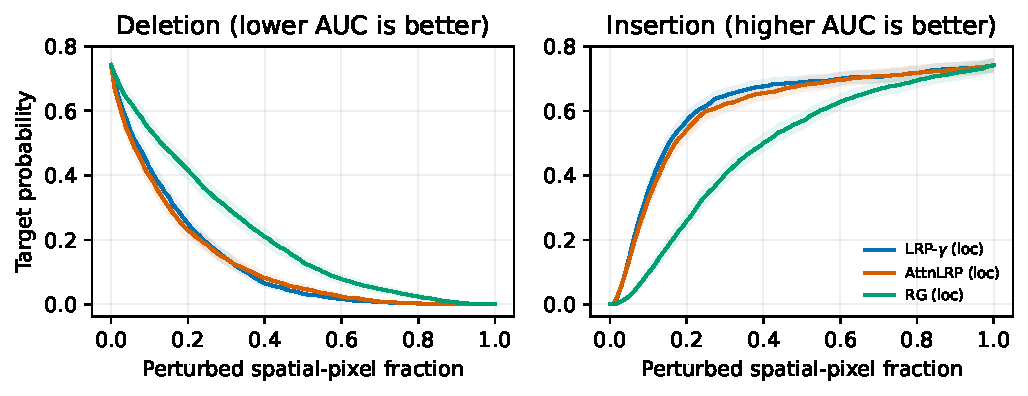
\includegraphics[width=.95\linewidth]{figures/rebuttal/full_auc_probabilities_selected.pdf}\\[.4em]
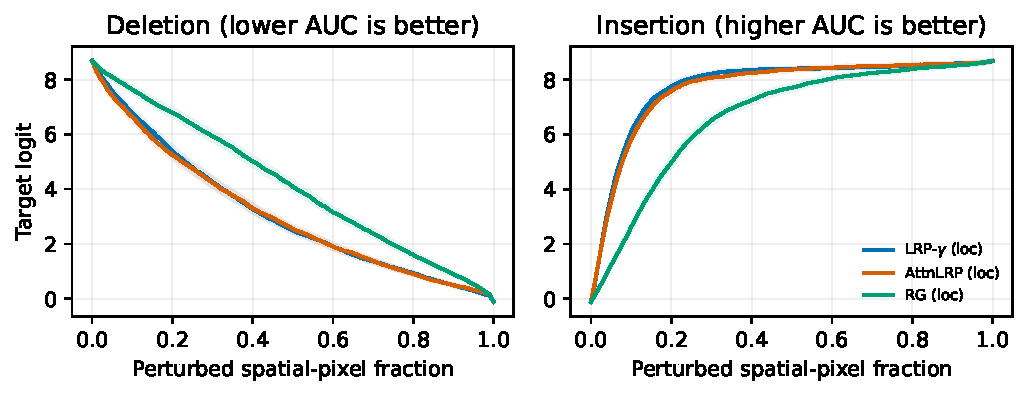
\includegraphics[width=.95\linewidth]{figures/rebuttal/full_auc_logits_selected.pdf}
\caption{Mean full deletion and insertion curves for localization-selected ViT-B/16 rows, using target probabilities (top) and raw target logits (bottom). Shading denotes pointwise image-bootstrap 95\% intervals.}
\label{fig:rebuttal-full-auc}
\end{figure}

\section{Robustness Controls}\label{app:rebuttal-robustness}

The ViT full-test robustness evaluation covers the validation-selected localization mode on all 565 images, using 50 image-keyed Uniform$[-0.2,0.2]$ perturbations in normalized input coordinates and 10,000 paired image resamples (seed 42). Validation selected $\lambda_{\mathrm{sm}}=-50$ at the fixed localization center. Compared with zero risk, MaxS changes from $.6850$ to $.6013$, AvgS from $.4447$ to $.3272$, while AL falls from $.6706$ to $.5204$. Thus lower sensitivity accompanies a substantial localization cost in this selected mode.

VGG-16 uses a gate-matched decomposition at the anchor. The first step changes a hard gate to a probit gate with $\lambda=0$; the second varies only $\lambda$ under that probit gate; the combined contrast compares the original hard-gate zero-risk row with the selected probit $\lambda=-2$ row. The table reports held-out means and paired differences, with 10,000 image-bootstrap resamples. The coefficient-only sensitivity gain incurs a small AL cost; the combined AL interval includes zero. This comparison isolates a selection-dependent effect and does not establish general robustness superiority.

\begin{table}[!ht]
\centering\small
\setlength{\tabcolsep}{4pt}
\begin{tabular}{>{\raggedright\arraybackslash}p{2.4cm}p{4.2cm}p{4.2cm}p{4.2cm}}
\toprule
Contrast & MaxS $\downarrow$ & AvgS $\downarrow$ & AL $\uparrow$ \\
\midrule
ViT loc, $\tau=.4,\varepsilon=.1$; $\lambda_{sm}:0\to-50$ & \shortstack{$.6850\to.6013$\\$\Delta=-.0837$\\$[-.1250,-.0419]$} & \shortstack{$.4447\to.3272$\\$\Delta=-.1176$\\$[-.1365,-.0985]$} & \shortstack{$.6706\to.5204$\\$\Delta=-.1502$\\$[-.1689,-.1322]$} \\
VGG anchor, gate only & \shortstack{$.5546\to.5265$\\$\Delta=-.0281$\\$[-.0330,-.0234]$} & \shortstack{$.4005\to.3714$\\$\Delta=-.0291$\\$[-.0317,-.0267]$} & \shortstack{$.6190\to.6207$\\$\Delta=+.0017$\\$[-.0002,+.0037]$} \\
VGG anchor, probit $\lambda:0\to-2$ & \shortstack{$.5265\to.4865$\\$\Delta=-.0400$\\$[-.0540,-.0264]$} & \shortstack{$.3714\to.3197$\\$\Delta=-.0518$\\$[-.0577,-.0460]$} & \shortstack{$.6207\to.6107$\\$\Delta=-.0100$\\$[-.0178,-.0021]$} \\
VGG anchor, combined & \shortstack{$.5546\to.4865$\\$\Delta=-.0680$\\$[-.0832,-.0532]$} & \shortstack{$.4005\to.3197$\\$\Delta=-.0808$\\$[-.0884,-.0737]$} & \shortstack{$.6190\to.6107$\\$\Delta=-.0083$\\$[-.0178,+.0013]$} \\
\bottomrule
\end{tabular}
\caption{Validation-selected risk contrasts on the full 565-image test set. Each cell gives both means, their difference (right minus left), and its paired 95\% interval. The ViT result is the selected localization-mode coefficient versus zero risk; VGG contrasts separate gate, coefficient and combined effects.}
\label{tab:rebuttal-risk}
\end{table}

The noise-protocol panel is a validation-only check of the ViT localization center ($n=50$). It crosses uniform and variance-matched Gaussian noise, $r\in\{.05,.1,.2\}$, and nested draw counts $\{10,25,50,100,200\}$, producing 30 correlated settings. For each setting, the risk-selected $\lambda_{sm}=-50$ is compared with zero risk using paired image intervals; intervals are unadjusted. MaxS, AvgS and 95th-percentile sensitivity means favor risk aversion in all 30 settings; their intervals exclude zero in 10, 30 and 19 settings, respectively. Cosine similarity favors risk aversion in all 30 settings, with intervals excluding zero in 10. Spearman similarity favors zero risk in all 30 settings, with intervals excluding zero in all 30. Top-10\% overlap means favor zero risk in all 30 settings, with intervals excluding zero in 10. Normalized-mass total variation favors risk aversion in 8 settings, with no interval excluding zero. These outcomes show that sensitivity and rank-based robustness diagnostics need not agree.

\section{Stopping-Game Pooling and Signed-Gradient Controls}\label{app:rebuttal-sg}

The submitted stopping-game (SG) benchmark exports the positive-player/positive-input (\texttt{pp}) component, not the signed occupation difference that recovers the input gradient. The original-forward pooling control caches max-pooling winners from the ordinary model forward and reuses them in the decomposed pass, keeping the submitted readout and all other settings fixed. On the 50-image VGG-16 validation split, the three configurations have identical PG, TK and Selectivity; paired intervals for AL, PF$_5$, PF$_{20}$, MaxS and AvgS contain zero except a $10^{-6}$ MaxS shift. This shows that pooling-index drift has negligible effect on the reported validation metrics at their precision. It is a diagnostic, not an equivalence test or a test-set result.

Separately, under per-layer numerical centering and cached original-forward pooling, the signed SG result matches autograd on all 50 validation images to a maximum relative $\ell_2$ error of $6.581\times10^{-7}$ with the theorem's strict ReLU-zero convention in float32; float64 reaches machine precision. The implementation's non-strict zero gate has larger float32 error ($2.873\times10^{-4}$ relative), while no exact-zero gate occurs in the float64 pass. Centering preserves the signed difference in exact arithmetic but changes individual components. This audit verifies the signed identity; it does not convert the submitted \texttt{pp} benchmark into a gradient benchmark.

\begin{table}[!ht]
\centering\small
\setlength{\tabcolsep}{3pt}
\begin{tabularx}{\linewidth}{>{\raggedright\arraybackslash}p{1.8cm}*{3}{>{\raggedright\arraybackslash}X}}
\toprule
Metric & Hard gate $\lambda=0$ & Localization-selected & Faithfulness-selected \\
\midrule
AL & \shortstack[l]{R/C: .5406/.5406\\$\Delta=-3.74\mathrm{e}{-07}$\\$[-1.46\mathrm{e}{-06},+4.31\mathrm{e}{-07}]$} & \shortstack[l]{R/C: .5681/.5681\\$\Delta=+4.04\mathrm{e}{-08}$\\$[-1.72\mathrm{e}{-07},+3.02\mathrm{e}{-07}]$} & \shortstack[l]{R/C: .5609/.5609\\$\Delta=+2.65\mathrm{e}{-08}$\\$[-3.34\mathrm{e}{-08},+1.20\mathrm{e}{-07}]$} \\
PG & \shortstack[l]{.7600/.7600\\$\Delta=+0.0000$\\$[+0.0000,+0.0000]$} & \shortstack[l]{.8800/.8800\\$\Delta=+0.0000$\\$[+0.0000,+0.0000]$} & \shortstack[l]{.7800/.7800\\$\Delta=+0.0000$\\$[+0.0000,+0.0000]$} \\
TK & \shortstack[l]{.7491/.7491\\$\Delta=+0.0000$\\$[+0.0000,+0.0000]$} & \shortstack[l]{.7306/.7306\\$\Delta=+0.0000$\\$[+0.0000,+0.0000]$} & \shortstack[l]{.7328/.7328\\$\Delta=+0.0000$\\$[+0.0000,+0.0000]$} \\
PF$_5$ & \shortstack[l]{17.396/17.395\\$\Delta=-0.002$\\$[-0.004,+4.37\mathrm{e}{-04}]$} & \shortstack[l]{16.339/16.341\\$\Delta=+0.001$\\$[-7.27\mathrm{e}{-05},+0.003]$} & \shortstack[l]{16.228/16.229\\$\Delta=+0.001$\\$[-0.001,+0.003]$} \\
PF$_{20}$ & \shortstack[l]{13.721/13.720\\$\Delta=-0.001$\\$[-0.002,+3.06\mathrm{e}{-04}]$} & \shortstack[l]{12.461/12.460\\$\Delta=-4.05\mathrm{e}{-04}$\\$[-0.001,+4.15\mathrm{e}{-04}]$} & \shortstack[l]{12.119/12.119\\$\Delta=+9.77\mathrm{e}{-05}$\\$[-0.001,+0.001]$} \\
Selectivity & \shortstack[l]{6.595/6.595\\$\Delta=+0.000$\\$[+0.000,+0.000]$} & \shortstack[l]{6.008/6.008\\$\Delta=+0.000$\\$[+0.000,+0.000]$} & \shortstack[l]{6.021/6.021\\$\Delta=+0.000$\\$[+0.000,+0.000]$} \\
MaxS & \shortstack[l]{.3758/.3758\\$\Delta=+6.69\mathrm{e}{-06}$\\$[-2.39\mathrm{e}{-06},+2.18\mathrm{e}{-05}]$} & \shortstack[l]{.2900/.2900\\$\Delta=+1.00\mathrm{e}{-06}$\\$[+2.01\mathrm{e}{-07},+1.96\mathrm{e}{-06}]$} & \shortstack[l]{.5315/.5315\\$\Delta=+3.69\mathrm{e}{-06}$\\$[-7.39\mathrm{e}{-06},+2.02\mathrm{e}{-05}]$} \\
AvgS & \shortstack[l]{.2845/.2845\\$\Delta=-1.28\mathrm{e}{-06}$\\$[-3.33\mathrm{e}{-06},+7.52\mathrm{e}{-07}]$} & \shortstack[l]{.1987/.1987\\$\Delta=+5.66\mathrm{e}{-07}$\\$[-2.68\mathrm{e}{-07},+1.51\mathrm{e}{-06}]$} & \shortstack[l]{.4180/.4179\\$\Delta=-2.01\mathrm{e}{-06}$\\$[-6.06\mathrm{e}{-06},+4.16\mathrm{e}{-07}]$} \\
$t$/img & \shortstack[l]{.074/.073\\$\Delta=-.001$\\$[-.002,-.001]$} & \shortstack[l]{.070/.074\\$\Delta=+.003$\\$[+.003,+.004]$} & \shortstack[l]{.070/.073\\$\Delta=+.003$\\$[+.003,+.003]$} \\
\bottomrule
\end{tabularx}

\caption{VGG-16 SG original-forward max-pooling control on the 50-image validation split. Each cell lists recompute/cached means followed by the paired cached-minus-recompute difference and its interval.}
\label{tab:rebuttal-sg-pooling}
\end{table}

\begin{changed}
\section{Routing-Game \texorpdfstring{$\alpha\beta$}{alpha-beta}-LRP Recovery}\label{app:rebuttal-rg}

We compare RG at $\tau=1$, with all policy deformations disabled, against independent $\alpha\beta$-LRP calculations. Each model uses three ImageNet-S validation images, $(\alpha,\beta)\in\{(1,0),(2,1)\}$ and $\varepsilon\in\{10^{-6},0.5\}$. A unit seed at the selected output logit fixes the relevance scale; errors compare the complete RGB relevance tensors before normalization or channel reduction. Bias shares are absorbed and each sign denominator receives its own $\varepsilon$, as in Theorem~\ref{ptnb:thm:ab-recovery}.

On pretrained VGG-16, the reference is Zennit's AlphaBeta rule, including signed first-layer contributions and ordinary max-pooling decisions. On pretrained ViT-B/16, an independent reverse recurrence covers the classifier, all twelve encoder blocks and the patch projection. It uses the observed QK-softmax, the composite Value rule of Theorem~\ref{ptnb:thm:attn-ab-recovery}, pass-through relevance at LayerNorm and GELU, and the implementation's full relevance to both addition operands (Section~\ref{ptnb:app:routing-skip}). Thus the ViT comparison verifies the stated local propagation rules throughout the model. Forward logits agree exactly on VGG-16 and within $7.11\times10^{-15}$ on ViT-B/16.

All end-to-end checks pass, reaching float64 relative errors below $3.3\times10^{-16}$ (Table~\ref{tab:rebuttal-rg-recovery}). Separately, fixed signed relevance seeds at each ViT attention--Value output test the composite rule in all twelve blocks: all 144 checks pass. These numerical checks use no reference-relevance injection and do not enter benchmark selection. Scripts, checkpoint hashes, image identifiers and per-run errors are retained with the code and in \nolinkurl{reports/evidence/routing-game-recovery/}.

\begin{table}[!ht]
\color{red}\centering\small
\begin{tabular}{llrrr}
\toprule
Model / scope & Precision & Checks & Max absolute error & Max relative $\ell_2$ error \\
\midrule
VGG-16 & float32 & 12 & $5.82\times10^{-10}$ & $4.11\times10^{-7}$ \\
VGG-16 & float64 & 12 & $4.34\times10^{-19}$ & $3.28\times10^{-16}$ \\
ViT-B/16 & float64 & 12 & $9.10\times10^{-13}$ & $3.19\times10^{-16}$ \\
ViT attention blocks & float64 & 144 & $5.26\times10^{-13}$ & $3.47\times10^{-14}$ \\
\bottomrule
\end{tabular}
\caption{RG recovery against independent $\alpha\beta$-LRP references on pretrained networks. Each entry is the worst error over the stated checks. End-to-end rows use unit output-logit seeds; the block row uses fixed signed relevance seeds.}
\label{tab:rebuttal-rg-recovery}
\end{table}
\end{changed}

\section{Checkpoint-Aligned Randomization and Local Hellinger Controls}\label{app:rebuttal-randomization}

The checkpoint-aligned ViT analysis evaluates map diagnostics and trajectory distance on the same 200 test images, dataset labels, model states and randomization conditions. Query/key/value projections remain pretrained in the cascade. Randomizing only the classifier head reduces top-1 accuracy from 88.5\% to zero and mean target probability from .7355 to .000932, while RG absolute-map rank similarity remains .999998; RG Hellinger distance is .769. Randomizing the last encoder block leaves map similarity at .999972 and raises Hellinger distance to .915. At the cascade endpoint, map similarity falls to .377 and survival-conditioned Hellinger reaches 1.000. The map projection can therefore remain nearly unchanged after predictive collapse, while the trajectory diagnostic registers changed routing. These results do not establish Hellinger as a predictor of accuracy or explanation quality.

Per-image associations are condition-dependent. At the cascade endpoint, RG Hellinger has Spearman correlation $-.203$ with RG map similarity (95\% CI $[-.333,-.072]$); head-only and last-block intervals include zero. The exploratory head-only association with absolute PF$_{20}$ change is $.273$ [$ .131,.403$], while other conditions include zero. Because randomization changes the classifier and logit scale, PF$_{20}$ change is not an independent explanation-quality endpoint. Local perturbations of the ViT classifier head produce increasing Hellinger distance as noise scale grows, while a small last-block attention-output perturbation produces much smaller distance; this is a local sensitivity diagnostic, not a quality calibration. Chapter~\ref{ch:trajectory} supplies the trajectory-space definitions and theorem scope.

\begin{table}[!ht]
\centering\scriptsize\setlength{\tabcolsep}{2pt}
\resizebox{\linewidth}{!}{\begin{tabular}{lrrrr}
\toprule
Condition & Top-1 acc. & Mean $p(y)$ & RG map $\rho(|a|)$ & $\mathrm{H}_{\mathrm{RG}}$ \\
\midrule
Identity & $88.5\%$ & $0.735504$ & $1.000000$ & $0.000$ \\
Head only & $0.0\%$ & $0.000932$ & $0.999998$ & $0.769$ \\
Last block & $0.0\%$ & $0.001016$ & $0.999972$ & $0.915$ \\
Cascade endpoint & $0.5\%$ & $0.000846$ & $0.377042$ & $0.963$ \\
\bottomrule
\end{tabular}
}
\caption{Prediction audit for the checkpoint-aligned ViT randomization controls ($n=200$ fixed test images).}
\label{tab:rebuttal-vit-prediction}
\end{table}

\begin{table}[!ht]
\centering\small\setlength{\tabcolsep}{3pt}
\begin{tabular}{@{}lccc@{}}
\toprule
Diagnostic & Head only & Through last block & Cascade endpoint \\
\midrule
Top-1 accuracy & $0.0\%$ & $0.0\%$ & $0.5\%$ \\
Mean target probability & $0.001$ & $0.001$ & $0.001$ \\
\midrule
\ac{sg}: $\mathrm H$ & $0.755\pm0.010$ & $0.886\pm0.004$ & $0.951\pm0.002$ \\
\ac{sg}: $\mathrm H_{\mathrm{surv}}$ & $0.755\pm0.010$ & $0.894\pm0.004$ & $1.000\pm0.000$ \\
\ac{rg}: $\mathrm H$ & $0.769\pm0.013$ & $0.915\pm0.005$ & $0.963\pm0.001$ \\
\ac{rg}: $\mathrm H_{\mathrm{surv}}$ & $0.770\pm0.013$ & $0.904\pm0.006$ & $1.000\pm0.000$ \\
\midrule
Gradient map $\rho(|a|)$ & $0.658\pm0.074$ & $0.655\pm0.074$ & $-0.035\pm0.134$ \\
\ac{rg} anchor map $\rho(|a|)$ & $1.000\pm0.000$ & $1.000\pm0.000$ & $0.377\pm0.238$ \\
\midrule
Association of \ac{rg} $\mathrm H$ with \ac{rg} map $\rho(|a|)$ & \shortstack{$+0.132$\\$[-0.010,+0.266]$} & \shortstack{$+0.059$\\$[-0.085,+0.199]$} & \shortstack{$-0.203$\\$[-0.333,-0.072]$} \\
\bottomrule
\end{tabular}

\caption{Checkpoint-aligned ViT map and trajectory diagnostics ($n=200$), transposed by diagnostic for legibility. Spearman associations are exploratory and unadjusted.}
\label{tab:rebuttal-vit-randomization}
\end{table}

\begin{table}[!ht]
\centering\small
\begin{tabular}{lrr}
\toprule
Perturbed module & Noise scale $s$ & $\mathrm{H}_{\mathrm{RG}}$ [95\% CI] \\
\midrule
Classifier head & $0.001$ & $0.001$ $[0.001,0.001]$ \\
Classifier head & $0.01$ & $0.011$ $[0.011,0.011]$ \\
Classifier head & $0.1$ & $0.090$ $[0.088,0.091]$ \\
Classifier head & $1$ & $0.500$ $[0.495,0.505]$ \\
Last-block attention output & $0.001$ & $0.001$ $[0.001,0.001]$ \\
\bottomrule
\end{tabular}

\caption{Local Hellinger response to controlled ViT weight perturbations.}
\label{tab:rebuttal-local-hellinger}
\end{table}




\chapter{Publication Provenance and Tool Use}\label{app:publication_provenance}

This thesis integrates two coauthored works with the thesis author as first author: \emph{Hidden Monotonicity}, a CVPR 2026 Highlight~\parencite{hiddenMono}, and the revised \emph{Playing the Network Backward} preprint, arXiv:2605.06212v2~\parencite{playingBackward2026}. It reuses their model-evaluation outputs and point estimates; the Pascal VOC intervals are recomputed by whole-image resampling, and the Holm-adjusted paired comparisons of the game-method tables are recomputed (Section~\ref{ptnb:app:stats}). The thesis places both papers in a common decomposition framework, which extends the Stopping Decomposition of the game paper, and adds theory, experiments and a partial Lean formalization.

Table~\ref{tab:provenance} separates the material taken from each paper from the work added in this thesis.

\begin{table}[htbp]
\centering\small
\begin{tabularx}{\linewidth}{@{}>{\raggedright\arraybackslash}p{3.2cm}>{\raggedright\arraybackslash}X@{}}
\toprule
Source & Material and location \\
\midrule
\emph{Hidden Monotonicity}~\parencite{hiddenMono} & The convexity and monotonicity criterion (Section~\ref{sec:convex_monotone_foundations}); the DC decomposition of ReLU networks by the maximum and identity pair (Section~\ref{sec:dc_splitting_relu}); stabilization and closed formulas for the shifted passes (Section~\ref{sec:stabilization_dc}); split rules for CNN components (Section~\ref{sec:cnn_decompositions}); SplitCAM, SplitLRP and SplitGrad (Section~\ref{sec:split_attribution_concept}); the sign-sorted product pair (starting point of Section~\ref{sec:multiplicative_splits}); the VGG-16 and ResNet-18 evaluation with its ablations, sanity check and runtime (Sections~\ref{sec:results_vgg}--\ref{sec:ablations}, Appendices~\ref{app:saliency}, \ref{app:p1_sanity}, \ref{app:p1_timing} and~\ref{app:ablation}); directly trained difference models on MNIST (Section~\ref{sec:dcinns}). \\
\addlinespace
\emph{Playing the Network Backward}~\parencite{playingBackward2026} & The Stopping Decomposition and the Softplus decomposition function (Sections~\ref{sec:stopping_decomposition} and~\ref{subsec:softplus_decomposition}); the Stopping Game and the Routing Game with the recovery of gradients and $\alpha\beta$-LRP, and the game modes (Chapter~\ref{ch:game_theory} without Section~\ref{ptnb:app:affine-readout}); the attention game (Section~\ref{ptnb:sec:attention}); layered Markov processes and the Hellinger distance between trajectory laws, with terminal-state disagreement and survival conditioning (Sections~\ref{ptnb:sec:lmp}--\ref{ptnb:sec:lmp-conditioned-survival}), and the pixel disagreement map (Section~\ref{sec:trajectory_pixel_map}); the trajectory experiments under input noise and under the two randomization cascades (Sections~\ref{ptnb:sec:hellinger-sanity}, \ref{ptnb:sec:lmp-experiments} and~\ref{ptnb:app:sanity-check} without the controls listed below); the evaluation on VGG-16, ResNet-50 and ViT-B/16 with Pascal VOC transfer and ablations (Sections~\ref{sec:results_vit} and~\ref{subsec:mode_ablation}, Appendices~\ref{app:game_timing} and~\ref{ptnb:app:results}) with its protocol (Appendices~\ref{ptnb:app:protocol} and~\ref{app:extended_protocol}). \\
\addlinespace
Theory added in the thesis & The definition of valid decompositions (Section~\ref{sec:general_decomposition_def})$^{\dagger}$; the profile criterion, the construction from absolute second derivatives and the closed formulas for smooth activations (Sections~\ref{sec:profile_criterion}, \ref{sec:dc_splitting_smooth} and~\ref{sec:closed_form_dc_activations}); the softmax pair (Section~\ref{sec:multivariate_dc_softmax}); the mixing family (Section~\ref{sec:mixing_decomposition})$^{\dagger}$; regularized decompositions (Section~\ref{sec:regularized_decompositions}); signed affine output logits in the Routing Game (Section~\ref{ptnb:app:affine-readout}); the polarized product pair, the LayerNorm pair and the DC decomposition of Transformers (Sections~\ref{sec:multiplicative_splits} and~\ref{sec:transformer_dc}); the two-step Markov process of the Routing Game, the local form of the Hellinger distance, and the effect of temperature and outside weight on it (Section~\ref{ptnb:sec:games-fit}). \\
\addlinespace
Experiments added in the thesis & SplitCAM on ViT-B/16 (Section~\ref{sec:vit-extension}); the gradient reconstruction check of the Transformer decomposition on ViT-B/16 (Section~\ref{app:transformer_dc_numeric}); the temperature comparison of Figure~\ref{fig:vit_temperature}, which includes $\tau=0.2$; recomputed Pascal VOC intervals and Holm-adjusted comparisons (Section~\ref{ptnb:app:stats}); the additional controls of Section~\ref{sec:additional-controls} and the matched-model and perturbation controls of the Hellinger cascade (Section~\ref{ptnb:sec:per-image-orthogonality})$^{\ddagger}$. \\
\addlinespace
Partial formalization & Lean~4 project covering the statements listed in Table~\ref{tab:lean_coverage} (Section~\ref{app:lean}). \\
\bottomrule
\end{tabularx}
\caption[Provenance of the thesis material]{Provenance of the thesis material. $^{\dagger}$In an earlier manuscript version of the game paper, not in arXiv~v2. $^{\ddagger}$Prepared for a later revision of the game paper, not in arXiv~v2.}
\label{tab:provenance}
\end{table}

\section{Author's Contribution}\label{app:author_contribution}

For both papers, I developed the theory and experiments, ran the experiments, and wrote all appendices and most text outside the introductions, collaborating with the coauthors listed in Section~\ref{sec:motivation}.

The next two sections disclose the use of AI tools, first in the preparation of the game paper and then in this thesis.

\section{Disclosure in the Revised Game Paper}
The revised game paper discloses the following for its preparation:
\begin{quote}
In this work, we used generative AI tools for implementing standard baseline methods and evaluation
code, for producing plots and tables of results, for drafting parts of the text, and for editing
(grammar, spelling, word choice, and reformatting).
We have not used generative AI tools to generate research ideas, to formulate the games, or to
produce the theorems and their proofs.
All AI-assisted code was reviewed and tested by the authors, including unit tests that check the
game-theoretic occupation measures against reference gradient and $\alpha\beta$-LRP
implementations; all AI-assisted text was checked by the authors for correctness, and every
reference was verified manually.
We take responsibility for the final content of this work, including text, claims, and artifacts
produced with the aid of generative AI.
\end{quote}

\section{AI Assistance in the Thesis Revision}
The November 2026 thesis revision used OpenAI Codex CLI for mathematical exploration, proof development, Lean implementation and checking, code review and repair, statistical reaggregation, and drafting and editing. Its session logs record CLI versions 0.166.0, 0.167.0, 0.167.1 and 0.171.0 and the model identifiers \texttt{gpt-6-astra} (main sessions), \texttt{gpt-6-luna} (delegated subtasks) and \texttt{gpt-6.1-sol} (one logged turn). The final revision used Anthropic's Claude Code, versions 2.1.323 to 2.1.331, with the model identifiers \texttt{claude-fable-5-2} and \texttt{claude-opus-5-5}: for drafting and editing text, for restructuring chapters and appendices and formatting tables, for checking reported numbers against the recorded experiment outputs and code, for checking proofs and correcting the Lean formalization, and for deriving and numerically checking the identities named below.

The division of the mathematical work is as follows. I developed all definitions, theorems and proofs of the two papers myself, and likewise the DC decomposition of smooth activations (Section~\ref{sec:dc_splitting_smooth}). Two parts of the mathematics were obtained with AI tools. The explicit convex, monotone softmax pair (Theorem~\ref{thm:softmax_dc_split}) was found by an AI tool; I checked its statement and proof. In Section~\ref{ptnb:sec:games-fit}, the local form~\eqref{ptnb:eq:h2-local} of the squared Hellinger distance and the row overlap of the Routing Game with its temperature expansion, \eqref{ptnb:eq:rg-row-overlap} and~\eqref{ptnb:eq:rg-row-local}, were derived with Claude Code and verified numerically. All other mathematical results of the thesis are my own, and for them the AI tools assisted with checking proofs and with the Lean formalization. These versions and model identifiers describe the thesis revision only; they do not identify tools used for the original papers. The quoted historical statement about theorem and proof development concerns the original paper, excluding this later thesis work.

The formalization folder contains audit files that restate the checked theorem types and print the axioms on which they depend; its README states the assumptions and the limits of the coverage. Lean certifies the stated propositions; source correspondence requires mathematical review, and kernel checks do not certify experiments.
